\documentclass[journal,9pt,a4paper]{IEEEtran}

\usepackage[english]{babel}
\usepackage[numbers]{natbib}
\usepackage{amssymb}
\usepackage{lipsum}
\usepackage{amsmath}
\usepackage{tikz}
\usepackage{subfigure}
\usepackage[scaled=0.99]{newtxmath}
\usepackage{array}
% \usepackage{caption}


% FOR CITE & REF
\usepackage{xcolor}
\definecolor{lightblue}{HTML}{0d7fac}
\usepackage[colorlinks]{hyperref}

\AtBeginDocument{
  \hypersetup{
    allcolors=lightblue}}

\renewcommand*{\thesection}{\Roman{section}}
\renewcommand*{\thesubsection}{\thesection.\Alph{subsection}}
\renewcommand*{\thesubsubsection}{\thesubsection.\arabic{subsubsection}}


\addto\extrasenglish{ 	\renewcommand{\sectionautorefname}{Sec.} 	\let\subsectionautorefname\sectionautorefname
\let\subsubsectionautorefname\sectionautorefname}

\begin{document}

\title{Uwb-based target localization and following system for UAV}

\author{Giorgio Pellegrini,~\IEEEmembership{giorgio.pellegrini@studenti.unitn.it, E.N. 239449}
\and
\\ Elias Fontanari,~\IEEEmembership{elias.fontanari@studenti.unitn.it, E.N. 231497}
        }
\maketitle
\thispagestyle{plain}
\pagestyle{plain}
\IEEEpeerreviewmaketitle

\begin{abstract}
Thanks to their increasingly compactness and versatility, Unmanned Aerial Vehicles (UAVs) usage in modern robotic tasks has grown in many different fields. Precision agriculture, environment exploration, search and rescue and fire fighting are only examples of the amount of possible UAVs applications. Among all, the interest in leader-follower tasks has grown, given its potential use (e.g. cinematographic shootings). In this work, a localization and following application is presented. The system is based on a new Ultra-wideband (UWB) kit, composed by a single and a double UWB antennas. Differently from other UWB-based leader-follower solutions, the proposed architecture uses not only ranging measures but also Angle of Arrival (AoA). Inherently it has all the advantages of UWB-based among visual-based system (low battery consumption and low computational effort), plus an already embedded way to localize a target in polar coordinate. The system performances were assessed by extensive simulations and by testing a real setup, using a motion capture system as ground truth. Although the UWB-pair kit presents high errors and non linearity for the AoA measurements, the tests have shown promising behaviour with an overall good following accuracy.
\end{abstract}

\section{Introduction}\label{INTRO}
UAVs are becoming useful partners in many situations and their low cost, compactness and versatility, has grown the researches interest in a lot of different application. For instance the effectiveness of UAVs usage was assessed in different application problems, such as crop disease detection\cite{cropdisdect}, complex environment exploration\cite{complenvexp}, fire monitoring, detection and fighting \cite{FireUAV}.\\
In all of the possible different applications, different control strategy are being used and refined in the years. One of the most investigated problem is target localization and following. This can be done using GPS position of both target and follower, but this solution remains too environmental restrictive, since in some situations, as for indoor application where satellites have poor precision or can even completely fail \cite{GPS-denied}, it is not suitable.\\
Nowadays most of the solutions to overcome this environment-related problems, are vision-based\cite{visualinertialrev}. They can rely on the flexibility in target changing and are already embedded in most of the commercial drones, for video shooting. The problems with this solutions is that they are based on computationally expensive image processing algorithm, and have high power consumption. Since computational limitation and battery duration are two well known UAVs problems\cite{UAVlimits}, the needing of more "light" solutions is researched.
A category of localization technology that shows high performance with a low power consumption and low computational effort, is the Radio Frequency (RF) based. These solutions make use of metrics such as Time of Arrival (ToA), Time Difference of Arrival (TDoA), Angle of Arrival (AoA), and Received Signal Strength (RSS), to perform localization. Some example of the technologies that can provides these measurements are Wi-Fi, Bluetooth, Ultra-Wideband (UWB), Zigbee, Radio Frequency Identification Devices (RFID), Long-Range Radio (LoRA), and cellular networks\cite{radiofreqloc}. Among all these possible solutions, UWB presents some unique characteristics like low-cost, low latency, low energy consumption, and centimeter-level accuracy. Moreover, as for the other RF-based application, UWB localization does not suffer from low-visibility conditions. For these reasons, many researchers in the field have studied localization, following and many other robotic applications using UWB-based architectures.\\
For instance, \citet{elderlycare} have developed an assisted PDoA positioning method for elderly care. They have developed a method to get rid of the Non-Line-Of-Sight (NLOS) error for elderly localization in elder-care structures. The method start with a first coarse localization with pure PDoA measures, subsequently refined by finding the actual antennas that are in Line-Of-Sight, providing an eventual NLOS compensation, and a final convex regression estimation.\\
A work more focused on following, is the one of \citet{Uwbbasedsol}, in which they have proposed a UWB-based solution, that fuse with a kalman filter, ranging measures coming from three UWB anchors, deployed on the drone in a triangular shape to avoid position ambiguities, with a linear target motion model. More specifically, they have shown that baseline length has an inversely proportional relationship with localization accuracy and with an Hardware-in-The-Loop simulation, and even with preliminary experimental-results on a commercial drone, they have demonstrate the functionality of the proposed following solution. In \cite{sidebyside} the authors present a side-by-side following method for a differential drive robot. They use PDoA measures developing a recursive least square parameter adaptation algorithm (RLS-PAA), which performs a control parameter regression while the target person is walking. On experimental test, considering a safe side distance of $0.5$ meters, they have achieved a true person-robot distance beyond $0.430$ meters for a circle trajectory and $0.482$ meters for a square trajectory, respectively, following quite well the shape of the target path.\\
To our knowledge, not a lot of work that make use of both TDoA and PDoA for localization, are present in the literature, with a complete absence of following application involving these quantity. An example could be the optimization-based position algorithm presented by \citet{tdoapdoa_optim}. The proposed method start with an initial location estimate, obtained by optimizing a TDOA cost function (considering a set of N measures obtained by N anchors deployed in the environment). Next, a PDOA, or a hybrid TDOA-PDOA cost function, is optimized using a particle swarm optimizer to obtain the final location estimate. This procedure has been proven to be effective in improving localization performance relative to pure TDOA methods.\\

Differently from the reviewed target following work \cite{Uwbbasedsol,sidebyside}, our work has the aim of asserting if raw TDoA and PDoA measure (from where range and AoA are calculated), can be enough to follow a target with enough accuracy w.r.t. the wanted strategy. Indeed no filtering, except of a PDoA averaging, is primarily performed to calculate the controls. To this end, we used a special kind of Ultra-wideband (UWB), pair of antennas. Developed by Qorvo, this kit is composed by a classic single UWB antenna and a double one, with their own Nordic companion board for the firmware. The kit was not developed and commercialized specifically to be compact and to be used on a moving robotic agent. In fact, it has a non negligible weight and encumbrance, that of course impact the overall system performance, both in power consumption and stability. However, since this work has the aim of studying the effectiveness of the TDoA/PDoA-based target following, this is not a problem. Thanks to the presence of an array of two antennas, the double UWB, which is deployed on the robotic agent, calculate both range and AoA w.r.t. the single UWB (i.e. the target). These two quantity are the minimum needed to localize the target w.r.t. the agent local reference frame in polar coordinates. In the proposed architecture, as can be seen in \autoref{INT:fig:drone_photo} the double UWB is mounted on a a compact 250 mm wheelbase UAV, whereas the target UWB could be kept by a human being or mounted on another robotic agent. The main contributions of this work are:
\begin{itemize}
    \item The development of an algorithm for target localization, given ranging and AoA measures;
    \item The development of a Gazebo Software-in-The-Loop simulation to evaluate the proposed following strategy;
    \item The Qorvo DW3 QM33 SDK UWB kit characterization;
    \item The development of a repeatable experimental setup, involving Motion Capture for ground truth, to test the described real system.
\end{itemize}
The rest of the paper is organized as follow: in \autoref{PRB_FORM} we formally introduce the problem, the sensed quantity, and the control law. In \autoref{ARCHIT} the quadcopter architecture, together with a description of the robot used as target and of the used motion capture system is exposed. Following, in \autoref{SIMULATION}, after a brief ROS2 introduction, we describe the simulated model of quadcopter and how it interacts with the simulated sensor, in the simulation environment. The implementation details, are instead exposed in \autoref{IMPLM_DET}, whereas in \autoref{UWB_CHAR} the UWB sensor kit is characterized. In \autoref{RESULTS} the results of both the simulation and the real test, are presented and compared and in \autoref{CONCLUSIONS} some conclusions and future improvements are discussed.

\begin{figure}
    \centering
    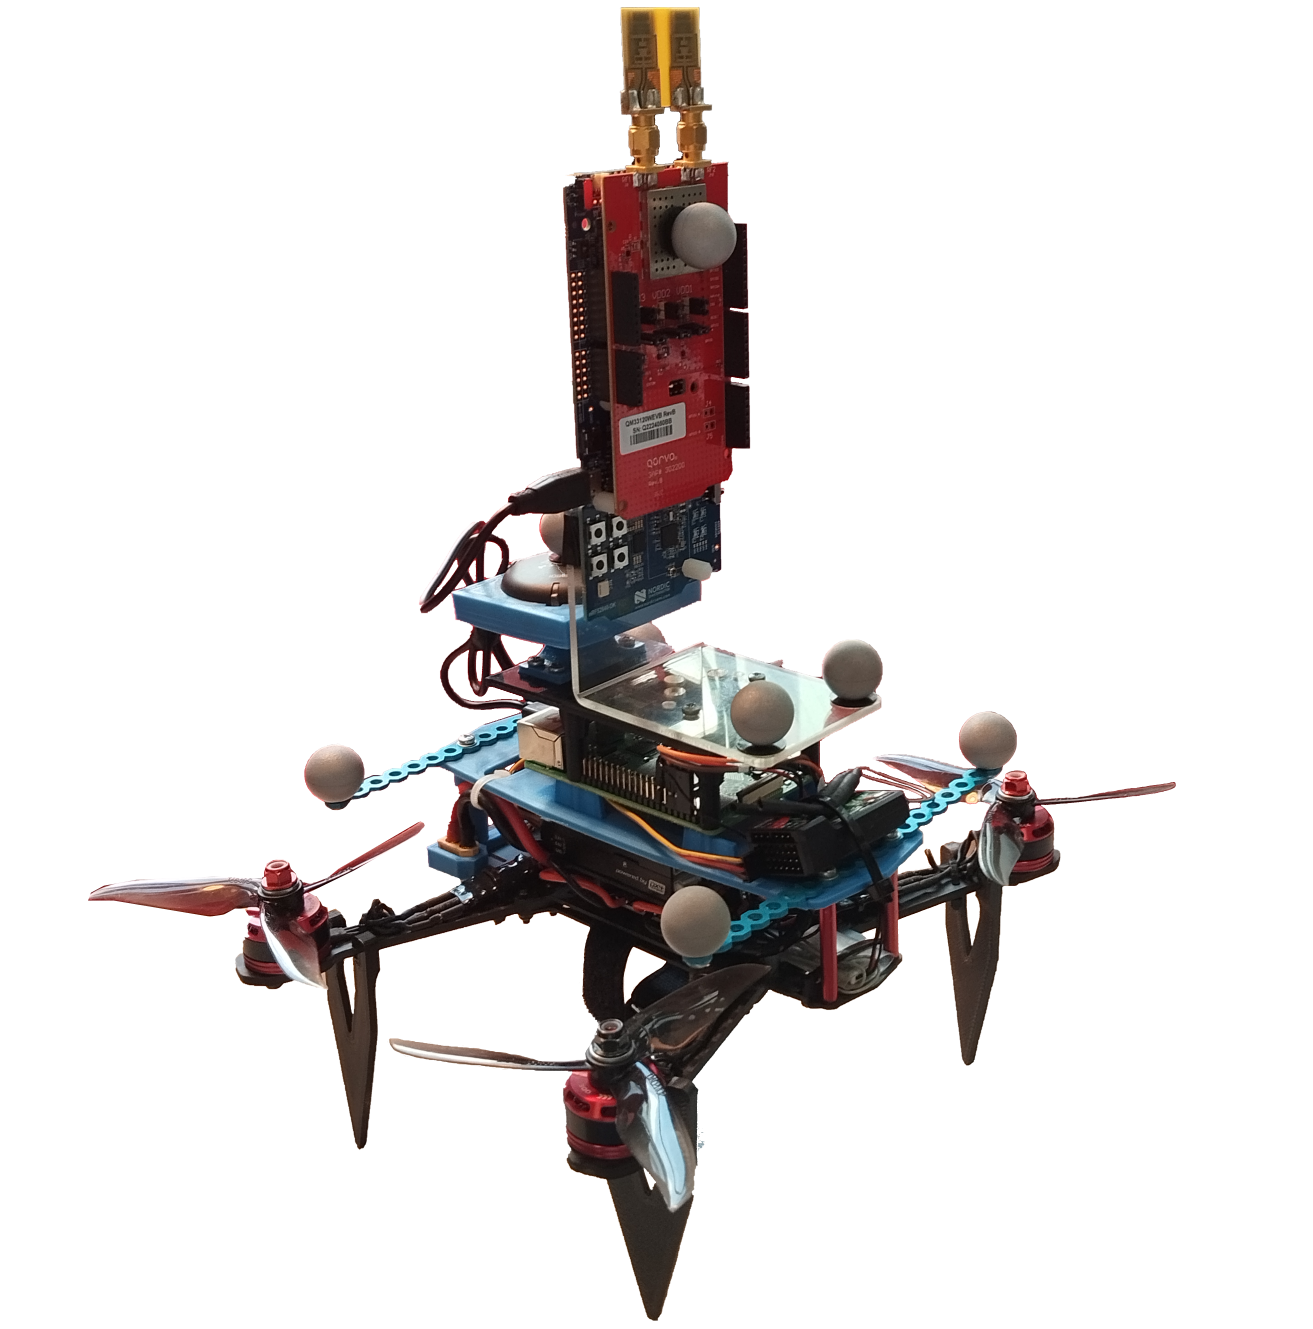
\includegraphics[width=0.4\textwidth]{images/drone_reale_tagliato.png}
    \caption{compact 250mm wheelbase Quadcopter used for the test. Is clearly visible the double antenna on top of the drone, as well as the marker used for the Mocap localization.}
    \label{INT:fig:drone_photo}
\end{figure}




\section{Problem formulation}\label{PRB_FORM}
\begin{figure}
    \centering
    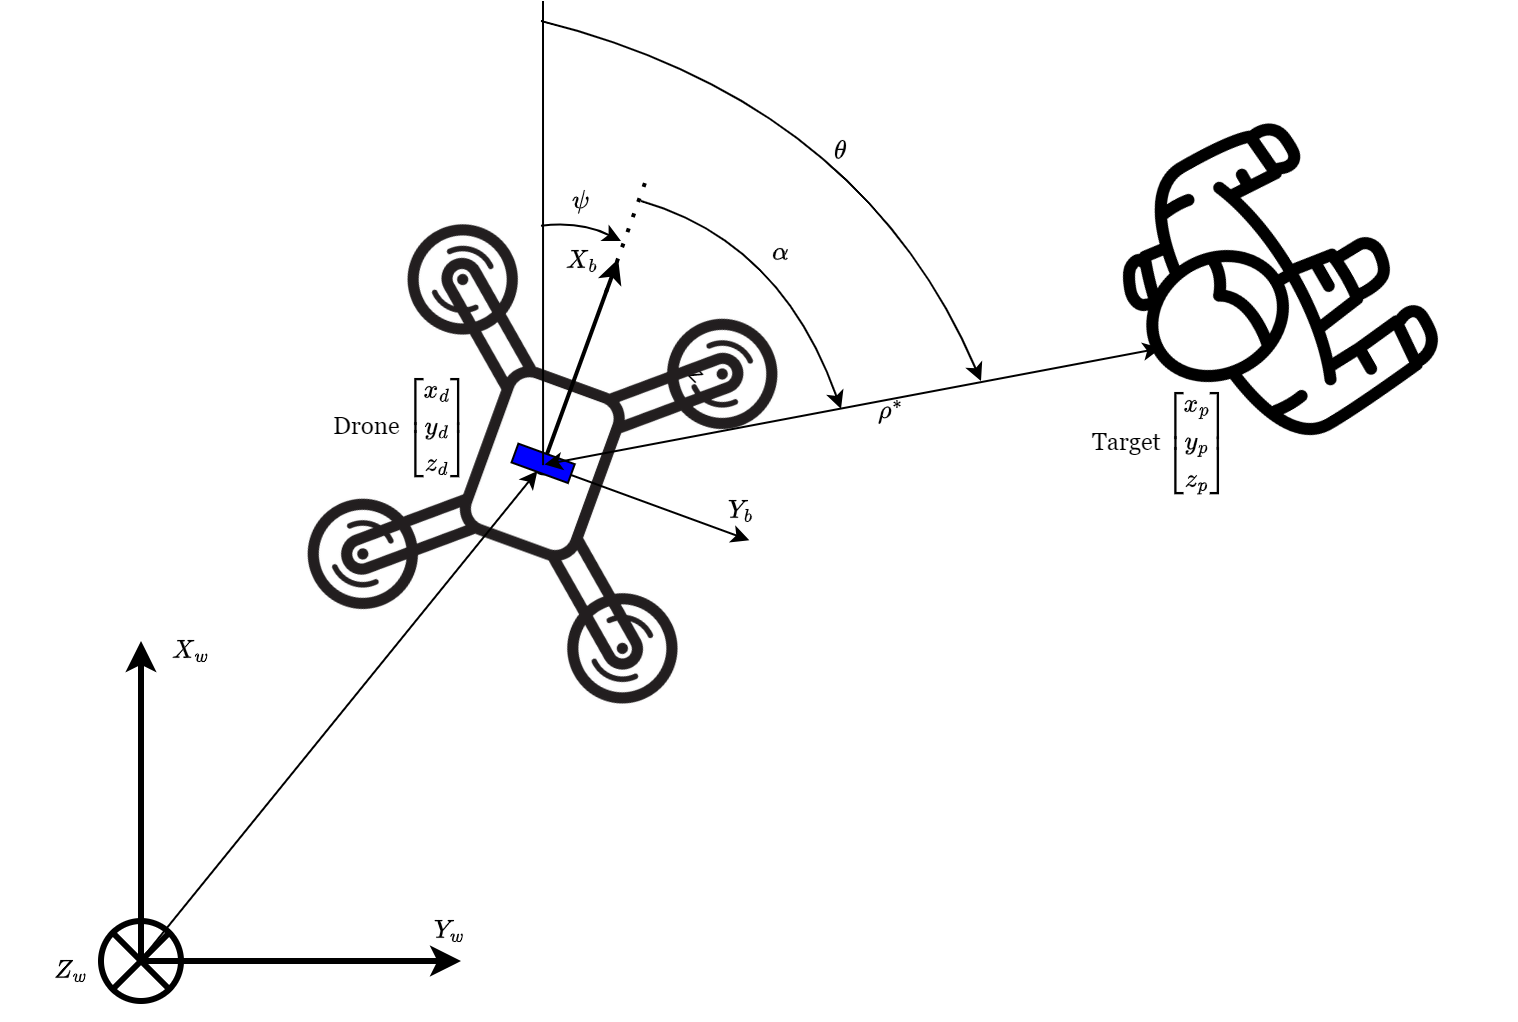
\includegraphics[width=0.47\textwidth]{images/Scheme_drone_tag.png}
    \caption{Application model scheme, in which the actual planar range $\rho^*$, the angles and both the drone local and the global reference frames, are highlighted. In blue is represented the double UWB antenna, deployed perpendicular to the drone's x direction.}
    \label{PRFOR:fig:dronetag_scheme}
\end{figure}


As previously introduced, the problem addressed in this work, is the classical \textit{leader-follower} application using relative range and angle. The policy to be maintained by the follower during the leader motion, is to stay at a constant distance (in the x-y plane), with an AoA of zero. The target (leader) is tracked using the single UWB (i.e. the tag), whereas the quadrotor is equipped with the double UWB (i.e. the follower). Let us define the coordinates of both tag \textbf{p} and follower \textbf{d}, in the global reference frame
\begin{equation}
\textbf{d} = \begin{bmatrix} x_d,y_d,z_d\end{bmatrix}^T \quad , \quad \textbf{p} = \begin{bmatrix} x_p,y_p,z_p\end{bmatrix}^T
\end{equation}
As said, the quantity delivered by the sensor are the range between the two antennas \textbf{$\rho$}, and the angle of arrival of the tag w.r.t. the follower \textbf{$\alpha$}. The range can be expressed as
\begin{equation}
    \rho = ||\mathbf{d} - \mathbf{p}||=\sqrt{(x_d - x_p)^2 + (y_d - y_p)^2 + (z_d - z_p)^2} + \eta = \Bar{\rho} + \eta
\end{equation}
Where $\eta$ is the measure uncertainty, which is supposed to be normally distributed, zero-mean and white, i.e $\eta \sim \mathcal{N}(0,\sigma_{\rho}^2)$. The variance of this quantity, is related to the UWB signal bandwidth and of course with the actual distance $\bar{\rho}$\cite{uwb_variance}. The range measurement is also affected by a bias introduced by the timestamp delay, which is different for each type of radio and is function of the actual distance $\bar{\rho}$\cite{UWBEvaluationOP}. Since in the proposed application the measured distance (without considering the initial conditions), should stay in a relatively strict band, a calibration in that band of interest, should be enough to mitigate the bias. Given that, the bias is supposed to be negligible. In the end, Line-of-sight (LOS) and negligible shadowing conditions are assumed, and so also Non-line-of-sight and shadowing sources of error\cite{UWBHumshadowing}, are neglected.\\
Clearly the measure obtained is the pure 3D range, which is not the wanted quantity, since the described policy is to maintain a certain distance in x-y plane. With the described configuration, it is not possible to directly obtain this value. But if we suppose that the quadrotor can collects measurements about its height $h$ w.r.t. to the ground (e.g. with a barometer, or any type of global positioning system) and assuming a fixed known value for the target height, is it possible to calculate the projection of the range in the x-y plane $\rho^*$. The assumption about the target height, can be simply made by knowing at which height the tag will be kept. Since in our test the tag is placed on a ground robotic agent, we have simply measured the height and saved as the constant $h_t$. In the end the projection $\rho^*$ can be calculated as follow:
\begin{equation}
    \rho^* = \sqrt{\rho^2 - \big( z_d - h_t\big)^2}
\end{equation}
where the double UWB antenna height $z_d = h + h_d$, i.e. the sum of the quadrotor height estimates $h$ and the relative height of the double antenna w.r.t. the flight controller $h_d$ (which is a construction constant).\\

For what concerns the angle of arrival, if we consider the double UWB face placed perpendicular to the x drone axis (as depicted in \autoref{PRFOR:fig:dronetag_scheme}) , it is possible to define the angle of arrival \textbf{$\alpha$} measured by the UWB, as follow:
\begin{equation}
    \alpha = \theta -\psi+ \xi
\end{equation}
where $\psi$ is the yaw orientation of the quadrotor, $\theta$ is the the geometric angle between the follower and the tag in the x-y plane and $\xi$ is the measure uncertainty, which, as for the range, is supposed to be normally distributed, zero-mean and white, that is $\xi \sim \mathcal{N}(0,\sigma_a^2)$. The same consideration and assumption done for the range, are also valid for the angle measure. This angle is obtained from the PDoA, that is the difference in phase of the signal received by the two antennas of the follower, by means of the following relation:
\begin{equation}\label{PRFOR:eq:aoa-pdod}
    \alpha = \arcsin \Bigg( \frac{\Delta\phi \cdot \lambda}{2\pi\cdot d} \Bigg)
\end{equation}
where $\Delta\phi$ is the PDoA, $\lambda$ is the signal wavelength and $d$ is the wheelbase between the two, in the double UWB, antennas. This conversion from PDoA to AoA is performed directly inside the Nordic companion board of the antenna, given that all the constant like $\lambda$ and $d$ are given in construction phase. Moreover, as will be later explained, this conversion is performed by knowing the calibration PDoA offset and the number of element over which averaging it. Both those quantities can be modified from serial port, to obtain the better possible value in the calibration phase.

\subsection{Control law}\label{control_law}
Let us define the wanted policy, as a vector with the wanted range, angle and height $r_w = \begin{bmatrix} \rho_w, \alpha_w, z_w\end{bmatrix}^T$ and the actual range, angle and height at time t $r_a(t) = \begin{bmatrix} \rho^* (t) , \alpha(t), z(t) \end{bmatrix}^T$. The control law has the scope of minimize and maintain low the difference $r_a - r_W$ in time. To do so three different control strategies are implied:
\begin{itemize}
    \item a PID controller to generate the x-y velocities setpoints
    \item a setpoint control for the yaw
    \item a setpoint control for the height
\end{itemize}
The PID controller is based on the difference between the actual measured range $\rho^*$ and the wanted value $\rho_w$, and by defining $d = \rho^* - \rho_w$, a scalar control value $V_s$ can be calculated:
\begin{equation}
    V_{s_k} = K_p\cdot d_k + K_d\cdot\Big(\frac{d_k - d_{k-1}}{\Delta t}\Big) + K_i\cdot I_{d_k}\Delta t
\end{equation}
Where $K_p$, $K_d$, $K_i$ are the proportional, derivative and integral gain respectively, $\Delta t$ is the time-step and $I_d$ is the cumulative integral value which can be defined as follow:
\[
    I_{d_k} = I_{d_{k-1}} + d_k
\]
The subscript $k$ defines the discrete $k$ instant at which the control is calculated. In order to obtain the actual x-y pair velocities, a last projection step has to be performed. Since the quantity $V_{s_k}$ represent the velocity to be applied in the direction of the target, the $V_{x_k}$ and $V_{y_k}$ control velocity, expressed in the global frame, can be obtained as follow:
\begin{equation}\label{PF:VELxy}
    \begin{bmatrix} V_{x_k} \\ V_{y_k} \end{bmatrix} = V_{s_k} \cdot \begin{bmatrix} \cos (\theta_k) & \sin (\theta_k) \end{bmatrix}^T
\end{equation}
where $\theta_k$, as already mentioned, is the geometric planar angle between the target and the drone and can be derived as:
\begin{equation}\label{PF:yawsp}
    \theta_k = \alpha_k +\psi_{k_{estim}}
\end{equation}
where $\psi_{k_{estim}}$ is the quadrotor yaw angle, estimated by the flight controller. Obviously this quantity is affected by both the uncertainty of the AoA measure $\alpha_k$ and of $\psi_{k_{estim}}$.\\
The two obtained control velocity, are fed to the flight controller as a velocity setpoint $V_{sp} = \begin{bmatrix} V_{x_k}, V_{y_k}, *\end{bmatrix}$, whereas $\theta$ is fed as the yaw setpoint, $\psi_{sp}$, to orient the drone toward the target. Lastly the height is controlled by feeding the flight controller with a position setpoint, $X_{sp} = \begin{bmatrix} *, *, z_w\end{bmatrix}$\footnote{The * simply means that the quantity is not given so not controlled}.
 




% In this leader-follower target problem, the leader can be anything movable entity while the follower is a quadcopter. The follower has the task of following the movements done by the leader, keeping a constant distance $r_{foll}$ in the plane x-y and a null angle $\theta_{foll}$, always in the same plane, w.r.t. the target. In order to do this the quadcopter needs to localize the target. We assume that the drone is equipped with all the sensors required to fly: GPS, IMU, compass, barometer as well with a flight controller that can properly fuse and filter all the sensor informations to localize itself globally and that can take as input setpoints (in position or velocity) and control the propellers to reach them. To localize the target globally is therefore sufficient a relative positioning system w.r.t. the follower, if its global pose it is known. For the relative positioning, we use a pair of UWB modules, and the one mounted on the drone has a pair of antennas while the one on the target is single. With this setup the planar azimuth angle can be estimated in addition to the ranging distance. The performance and the characterization of the UWB system will be discussed successively. \\
% With these informations, the PID control law that we adopted to compute the proper velocity setpoints expressed in the global frame to be sent periodically to the flight controller are calculated in this way:
% \begin{equation}\label{MOD:velocities}
% \begin{bmatrix}
%     v_{x} \\
%     v_{y}
% \end{bmatrix}
% = (k_{P} \cdot r_{P} + k_{D} \cdot r_{D} + k_{I} \cdot r_{I}) \cdot 
% \begin{bmatrix}
%     cos(\psi_{set})\\
%     sin(\psi_{set})
% \end{bmatrix}
% \end{equation}

% $k_{P}$, $k_{D}$ and $k_{I}$ are the chosen PID gains, while $\psi_{set}$ is the yaw commanded in order to orientate the front of the quad toward the target: 

% \begin{equation}\label{MOD:yaw}
%     \psi_{set} = \psi_{glob} + \theta_{UWB}
% \end{equation}


% \begin{equation}\label{MOD:controlPID}
% \begin{bmatrix}
%     r_{P}\\
%     r_{D}\\
%     r_{I} 
% \end{bmatrix} =
% \begin{bmatrix}
%     r_{xy} - r_{foll}\\
%      \frac{r_{P} - r_{P prev}}{dt}\\
%     r_{I} + r_{P} dt
% \end{bmatrix}
% \end{equation}
% The subscript UWB indicates informations that comes from the sensors, $dt$ indicates the period with which setpoints are sent and $\psi_{glob}$ is the estimated yaw in the global frame. The velocity in the z-axis is not reported since we assume that the the flight takes place at a constant height, $z_{fly}$ reached after a takeoff and the flight controller is able to maintain it. It is even assumed that the height of the tag $z_{tag}$ on the target does not change, so $r_{xy} = \sqrt{r_{UWB}^2 - (z_{fly}-z_{tag})^2}$. This control law will be tested in simulation and with real hardware to understand if it can be suitable and to evaluate its performance.


% Let us define the wanted policy, as a vector with the wanted range, angle and height $r_w = \begin{bmatrix} \rho_w, \alpha_w, z_w\end{bmatrix}^T$ and the actual range, angle and height at time t $r_a(t) = \begin{bmatrix} \rho^* (t) , \alpha(t), z(t) \end{bmatrix}^T$. The control law has the scope of minimize and maintain the difference $r_a - r_W$ in time as wanted, flying at constant height and keeping the quadcopter orientation pointed toward the target.\\ To do so three different control strategies are implied:

\section{Leader-follower system setup}\label{ARCHIT}
\begin{figure}
    \centering
    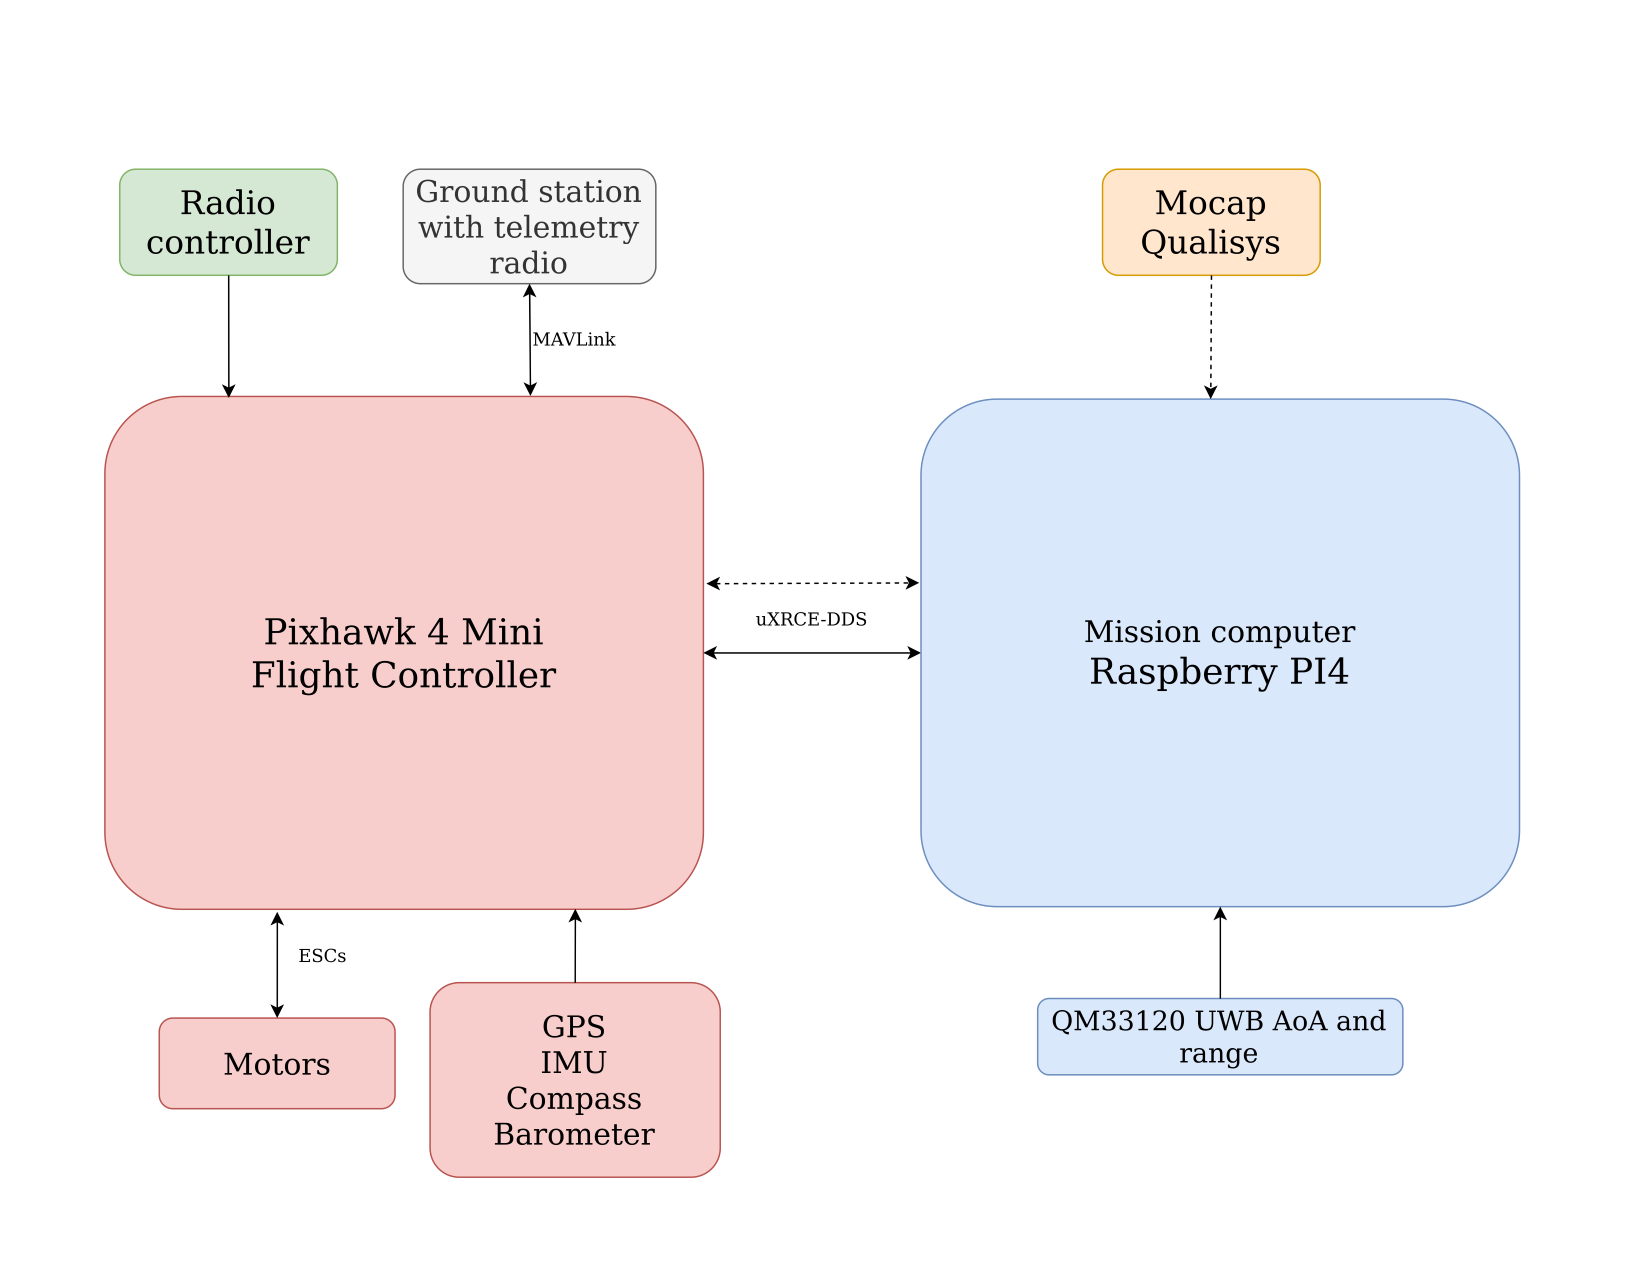
\includegraphics[width=0.45\textwidth]{images/FCA.png}
    \caption{Quadcopter architecture.}
    \label{ARC:fig_comp}
\end{figure}

\begin{figure}
    \centering
    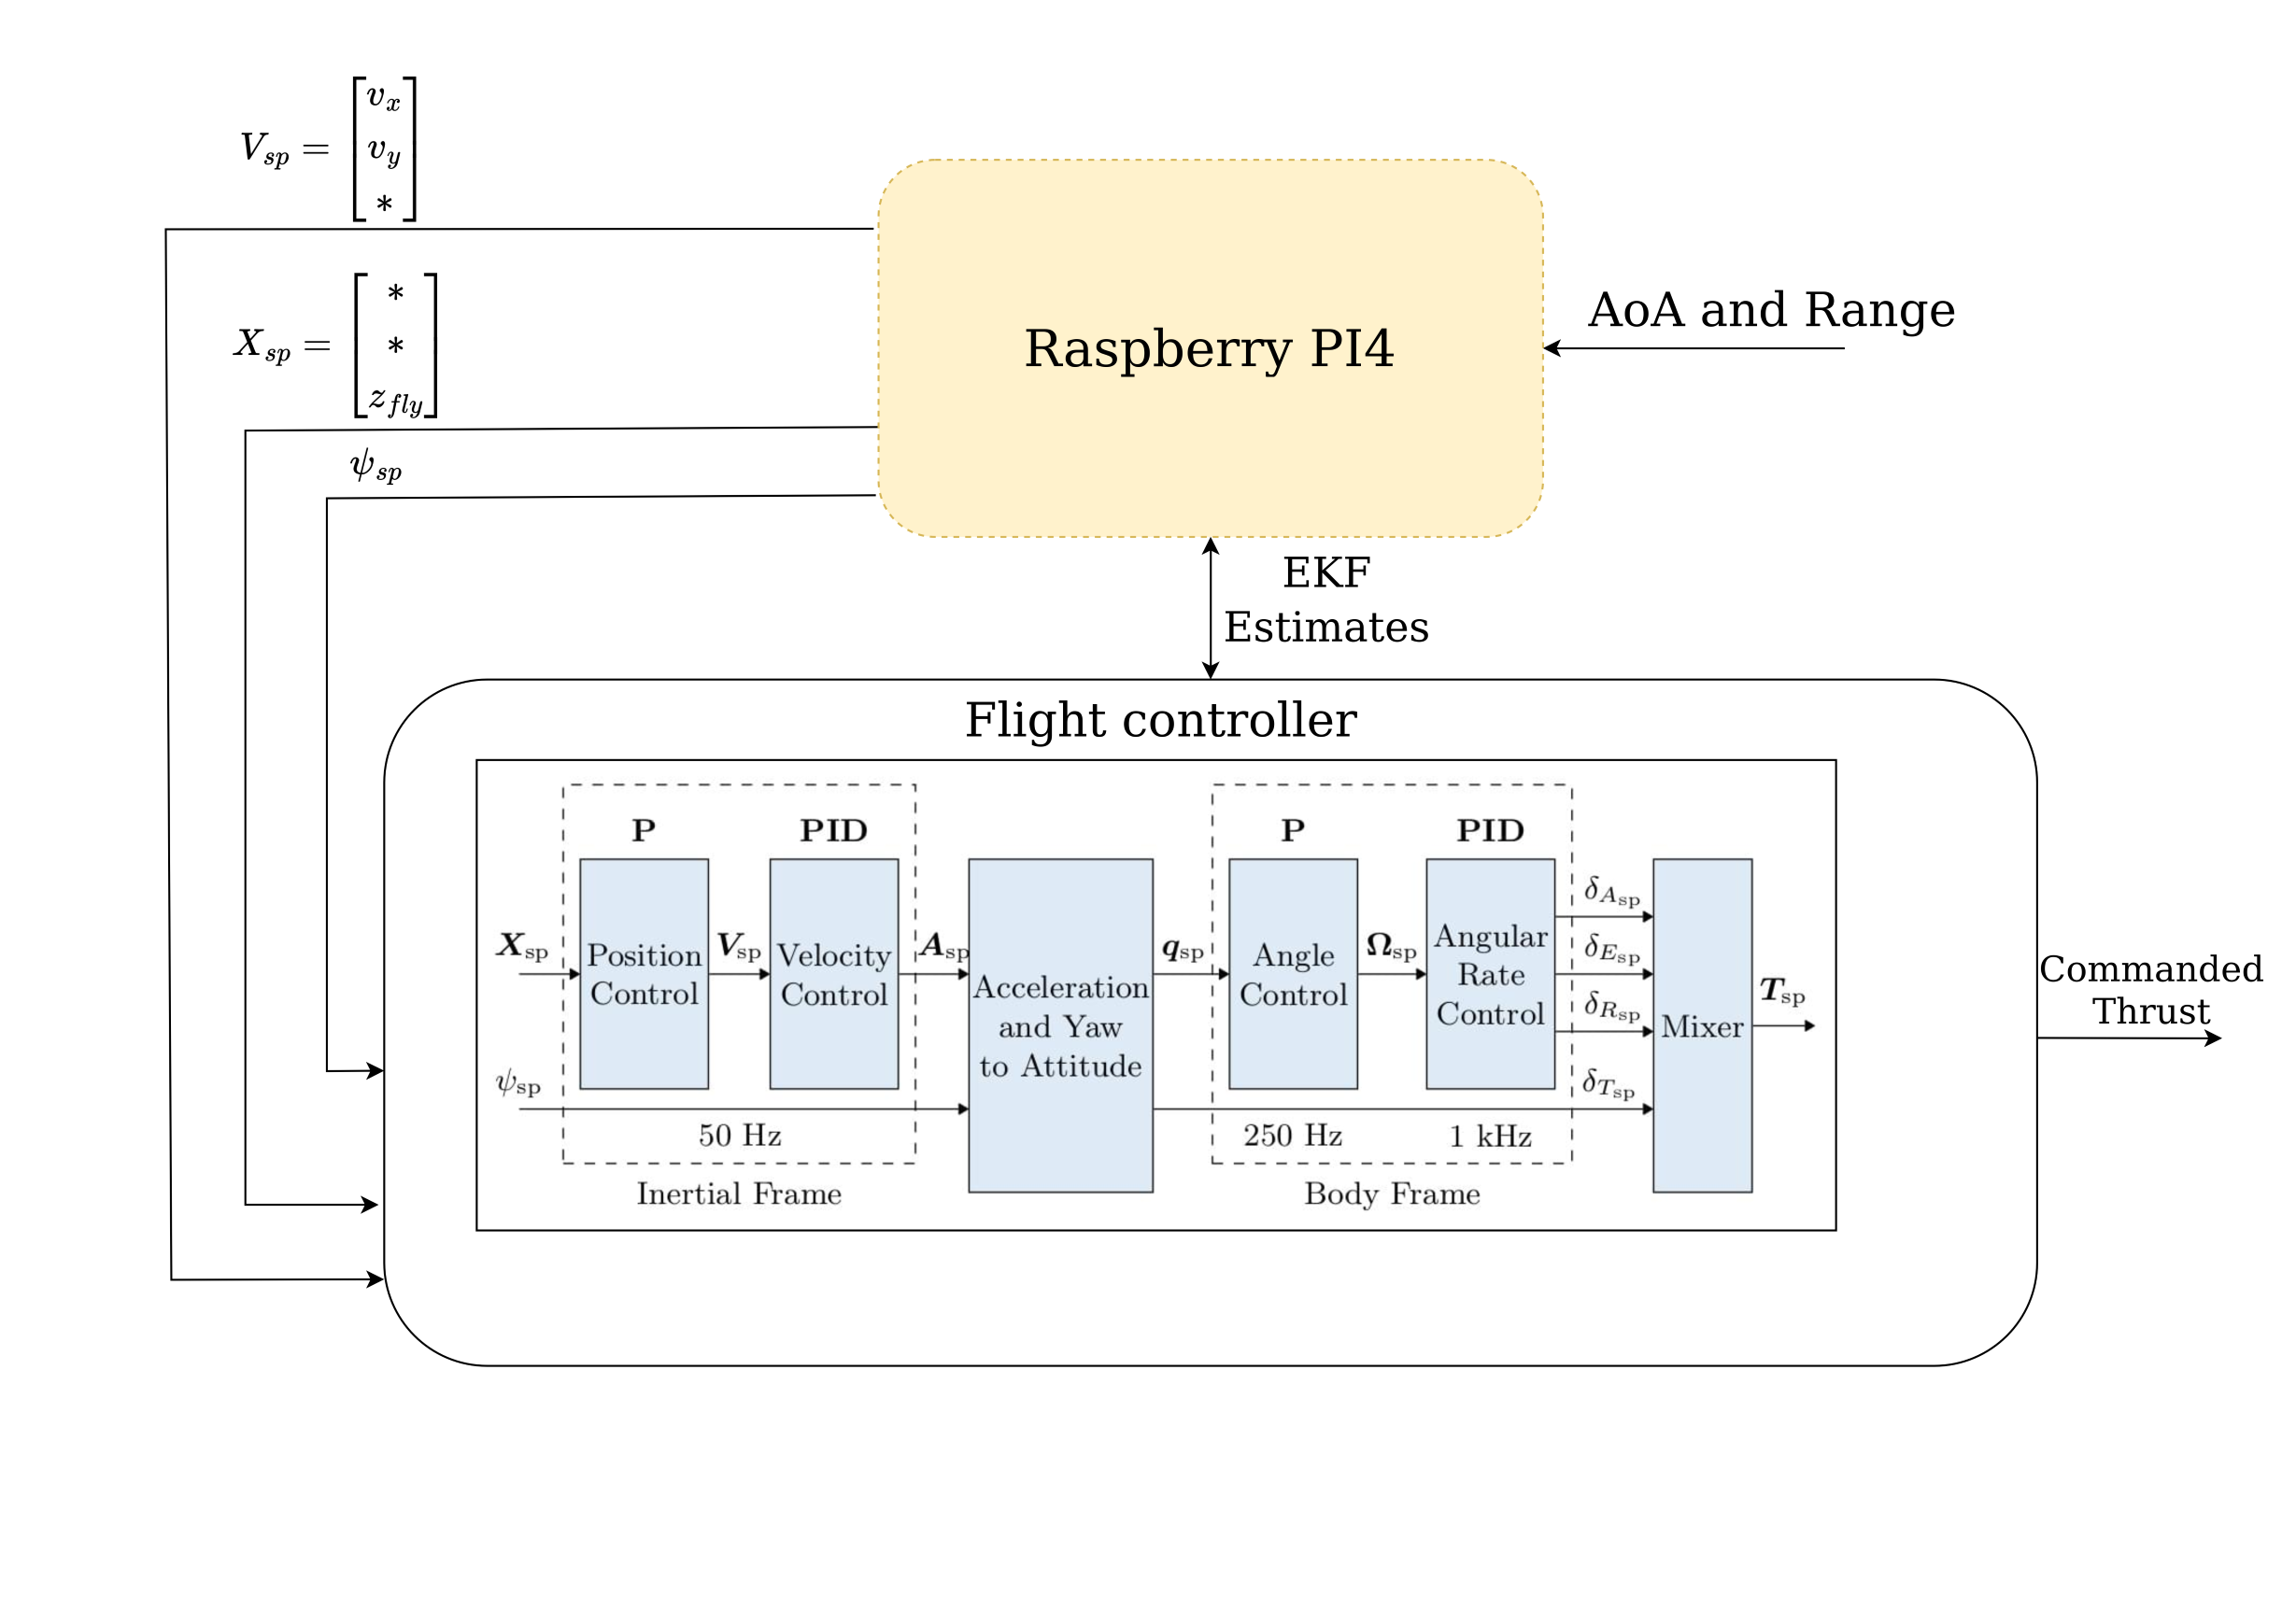
\includegraphics[width=0.45\textwidth]{images/Contr Diagram.png}
    \caption{Flight control loop: * stands for not controlled: if in \(X_{sp}\) it means that control computed starting from Velocity Control, if in \(V_{sp}\) computed by not empty Position Control input.}
    \label{ARC:fig_contr}
\end{figure}

In the proposed leader-follower application, the target carry a single antenna UWB transceiver while the chaser is a QAV250 quadcopter equipped with a Pixhawk4 Mini flight controller, a Raspberry Pi4 and a double antenna UWB transceiver that communicates through serial port to the mission computer, supplying to it range and angle of arrival of the target w.r.t. the drone.

\subsection{Quadcopter architecture}
The architecture and the interactions between the components of the vehicle are schematized in \autoref{ARC:fig_comp}.\\
The flight controller (FC) runs the PX4 Autopilot firmware, responsible for controlling propellers and for state estimates. The Raspberry using the received target location information and the drone state estimates, provides the control velocity setpoints, toghether with the yaw and the height setpoints (as explained in \autoref{control_law}), to the FC. The flight controller then, using a combination of nested P and PID controllers, converts the inputs in motor thrust commands (as depicted in figure \autoref{ARC:fig_contr} , using a combination of nested P and PID controller.\\

Since PX4 has the possibility of using a uXRCE-DDS middleware (a client running on the FC and an agent on the Raspberry) to allow uORB messages (that contains information such as command or veichle estimates and status) to be published and subscribed on a companion computer as they were ROS2 topics, the Raspberry can interact with the flight controller using these topics (better details about ROS2, topics and publishing/subscribing will be later exposed). The advantage of using the middleware ROS2 is a great flexibility, since all the devices connected to the network can access to all the topics published, even those of the FC interfaced to the Raspberry. In our case this is particularly useful, in order to integrate Motion capture as the global reference for the UAV, as it will be explained later, and of course to send the FC control inputs.

\subsection{Target}
To ensure that the UWB tag keeps a constant height during the motion and to avoid possible dangerous situations that involves human beings during testing, as target we used a customized differential drive lawn-mower robot \autoref{ARC:fig:tag_photo}, with the UWB tag rigidly mounted on it. During our tests a person was in charge of driving this DDR with a radio controller.

\begin{figure}
    \centering
    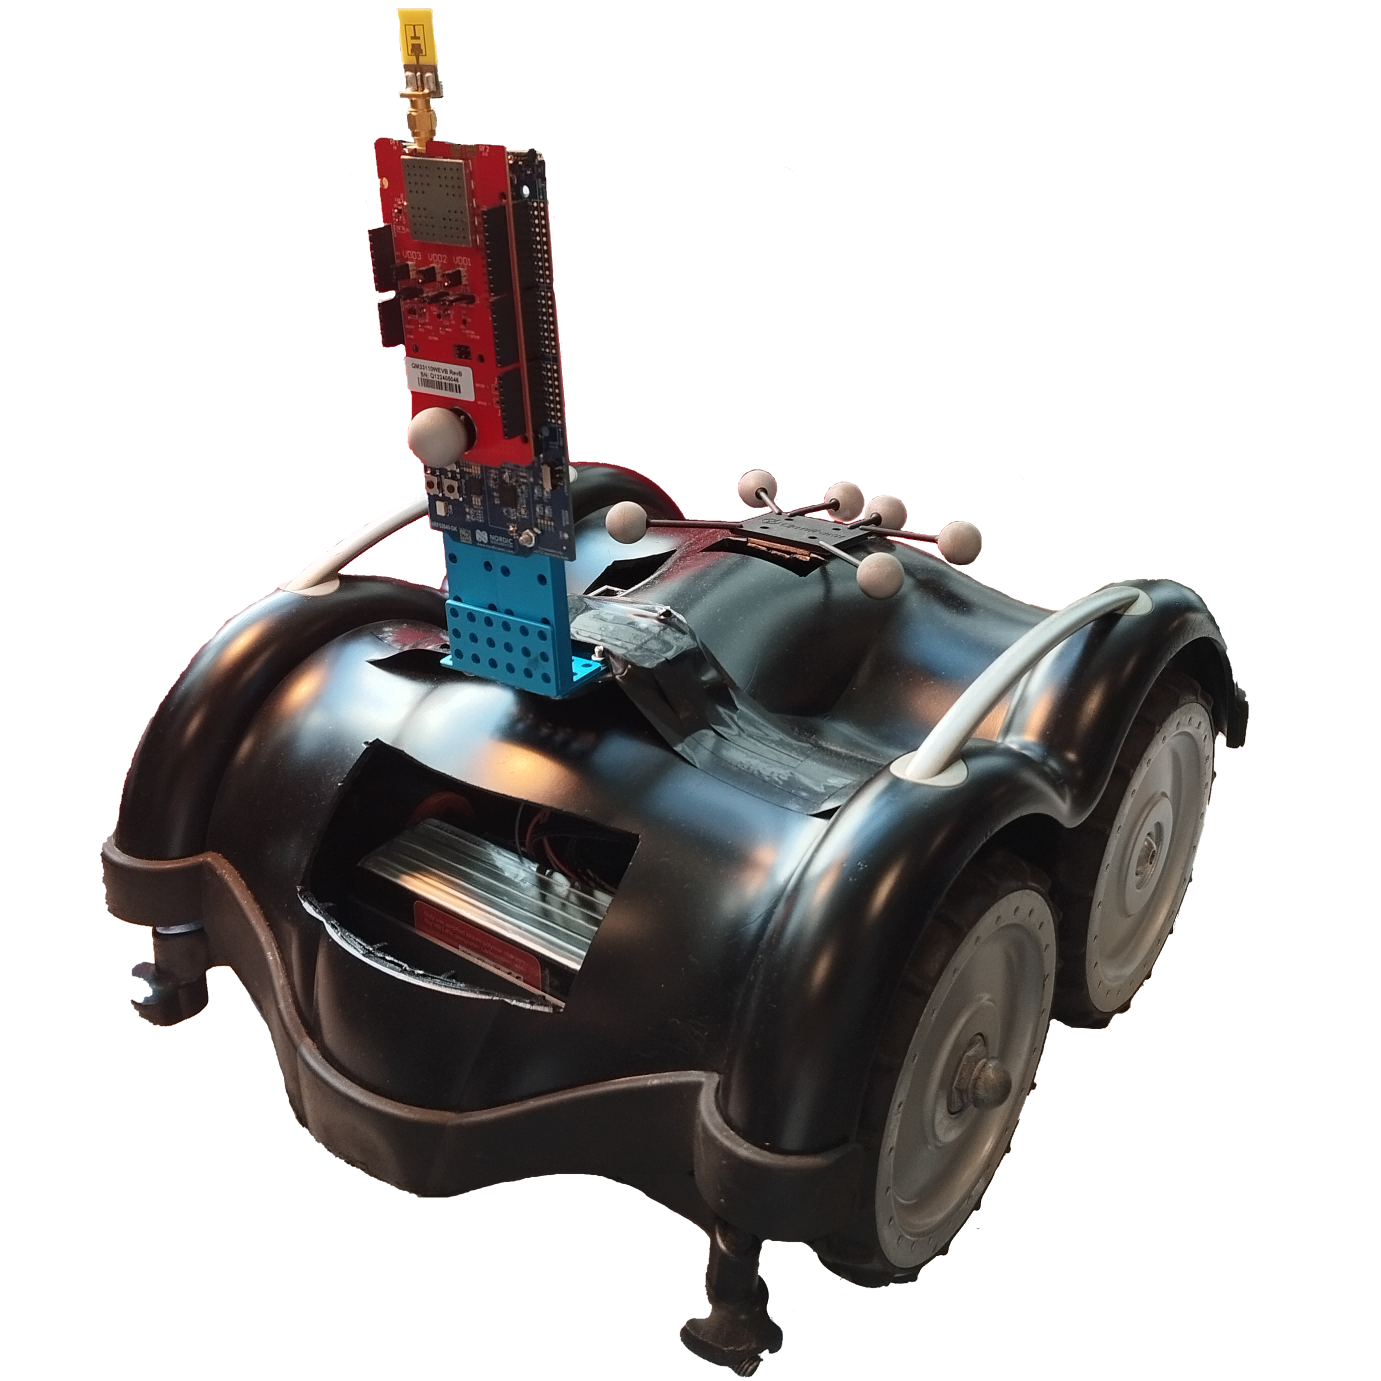
\includegraphics[width=0.4\textwidth]{images/target_reale_tagliato.png}
    \caption{DDR target. Is visible the mounted single antenna, as well as the presence of the Mocap markers, used to get his absolute position.}
    \label{ARC:fig:tag_photo}
\end{figure}

\subsection{Qualisys motion capture system}
In order to have a precise pose ground truth we performed our tests indoor in a dedicated room with a system of seven Qualisys Arqus cameras installed. The system is able to precisely locate the reflective markers that can be mounted on the bodies to track, using the different views of the cameras. To track a body, a fixed configuration of at least 3 markers has to be mounted on it. However, to avoid possible troubles with marker occlusions, is suggested to place more markers. In our case we obviously tracked the target and the quadcopter to evaluate their motion. \\
Since in indoor, GPS is not available, the quadcopter pose estimate done by the MoCap is used also as Global positioning, both in position and orientation. The way in which it is done will be explained in \autoref{Mocap details}. In addition we have disabled the compass and the barometer contribution to the vehicle's EKF, deactivating the related parameters in the flight controller firmware, since Mocap provides alone, a millimeter-level positioning precision. Beyond the uselessness, the reason of this deactivation lies in the indoor unreliability of these type measurements, due to environmental interference or misleading information (i.e. altitude and magnetic orientation have no meaning in the global reference frame of the Mocap lab).

\section{Simulation}\label{SIMULATION}
\begin{figure}
    \centering
    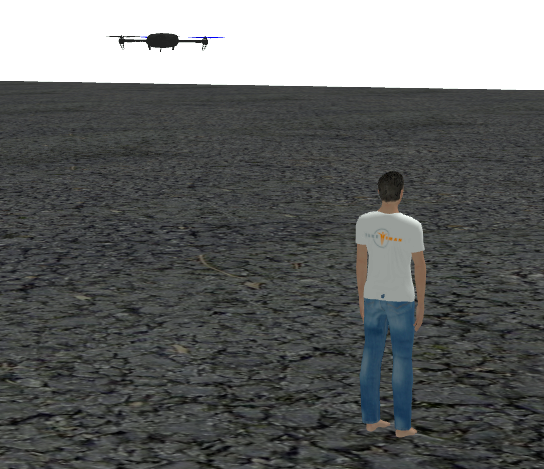
\includegraphics[width=0.4\textwidth]{images/screen_simulazione.png}
    \caption{Simulation's SITL image.}
    \label{SOL:fig:screensimulazione}
\end{figure}

\subsection{ROS2 Brief introduction}
Before diving into the simulation, is important to explain the ROS2 functioning. The Robot Operating System (ROS) is a set of software libraries and tools for building robot applications. A ROS2 application, can be seen as a network, or better a graph, composed by ROS2 elements, processing together at the same time. The principal ROS2 elements are the nodes, which are the actual computational elements. Each node can send and receive data from other nodes via topics, services, actions, or parameters. ROS2 Nodes can be software Robotic components, like the Flight controller, or can be user programmed. The base principle in ROS2 nodes communication is the pubblisher/subscriber protocol. For what concerns topics (which are the only communication medium used in this work), each node can be a publisher, so it can "change" the topic value, or a subscriber, so it can "read" the topic value. In this way, ROS2 is an effective communication interface between different hardware and software, with the only requirement of being connected to the same network. A representation example of a ROS2 network, is the one of our Simulation depicted and explained in \autoref{SIM:fig:nodism}.\\
A user programmed Node is typically defined inside the so called ROS2 packages, in which the Node executable can be interfaced with user defined topics and messages, or with some defined by others. For example the PX4 team have developed a series of packages in which they define all the messages topics, services and actions needed to fully interact with the flight controller (regardless if it is the simulated one or a real one, since they are equal in software). Packages can be programmed both in C++ or Python, and can be grouped together in ROS2 workspace. For better details, we refer to the ROS2 Documentation\cite{ros2doc}.

\begin{figure}
    \centering
    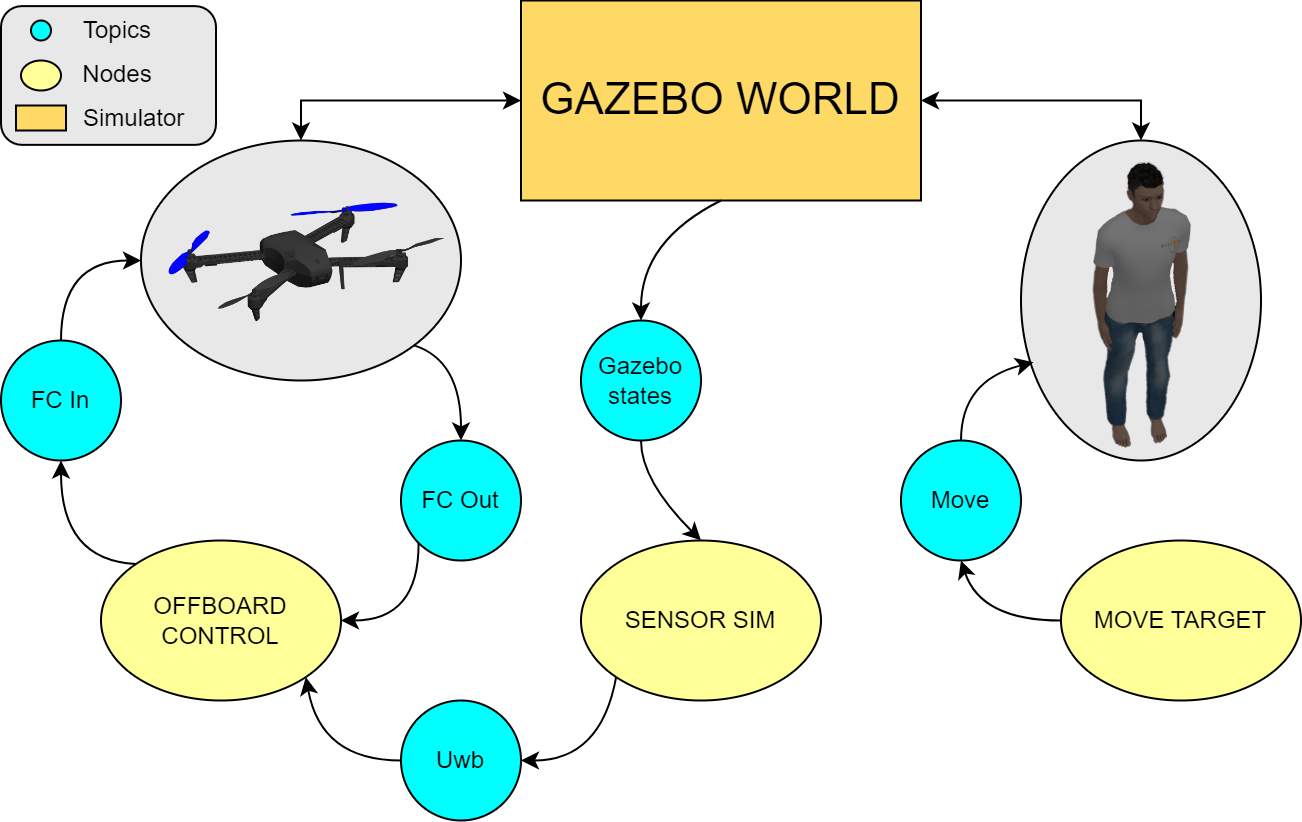
\includegraphics[width=0.45\textwidth]{images/nodi_simulazione.png}
    \caption{ROS2 simulation Network. The nodes (yellow ellipses) can be subscriber or publisher to the topics (light blue circles). In this way, for example, the offboard node can retrieve the drone's state estimates from the FC, and send to it the controls.}
    \label{SIM:fig:nodism}
\end{figure}

\subsection{Simulation}
To assess and validate the developed control law, is necessary to test it on a simulation that well resembles the reality.
This is possible conducting software in the loop simulations, with the same flight controller available as hardware and possibly with the same vehicle.
Working with the PX4 flight stack, as it is the one that runs on our flight controller, the best simulation environment to use is Gazebo, a graphic simulator with an accurate physics. It is also easily customizable through the use of plugins permitting to include other effects as the wind. Moreover, it interacts well with ROS2,  allowing for a lot of flexibility in use.\\
The vehicle on which we tested our control law in simulation is the Iris quadcopter, the main model for gazebo PX4 simulations (even though it is different from the one we used in real tests). This model guarantees a great level of simulation accuracy: the motors and the generated thrusts are modelled accurately using specific plugins, and even its navigation sensors are corrupted appropriately to be similar to real-case scenarios. Even the flight controller is simulated as the real one, having the same estimation algorithms, controller and characteristics.\\
To simulate the target we defined a simple object, with the appearance of a human, that can translate in the x and y direction. To make it move, we created a ROS2 node that publishes on the gazebo ROS2 topics the position of the target, making it move. To make it move at a certain speed and with the desired trajectory, nearby points are sent to gazebo at a constant rate.\\
To simulate the range and AoA sensor, it is necessary to know the global position in the gazebo world of both target and drone, together with the yaw of this last one. Once that these information are known, and in our case it is simply done with another ROS2 node that subscribes to the pose topic of the objects in gazebo, with simple geometric relations it is possible to determine the true angle and range and then corrupt them with noise, to simulate the sensor. In our simulations, we simply added normally distributed, zero mean and white noise to both quantities (referring to the values obtained in the characterization of the true sensor). This simulated sensor node, supplies the simulated sensor readings to the offboard-control node which, by accessing to the drone estimates, compute the velocity setpoints as in \eqref{PF:VELxy}, together with the yaw setpoint \eqref{PF:yawsp} and the position setpoint for the height control, sending them to the FC. It is interesting to note that, since the flight controller is fed via ROS2 even in the real case, the same offboard control node can be used in the real application, of course using the range and AoA measures given by the real UWB sensor. A Detailed scheme of the ROS2 network is presented in \autoref{SIM:fig:nodism}. Simulation results are exposed later, in \autoref{SIM_RES}.

\section{Implementation details}\label{IMPLM_DET}
In the following section, some details about the implementations will be exposed. For details about the source code, we refer to our git-hub repository \cite{git-repo}

\subsection{Offboard control node}
The heart of the following algorithm, as already mentioned, resides in the Raspberry Pi 4 and it is the offboard control node. In particular, the tasks that it performs are the following: 
\begin{itemize}
    \item when started, it subscribes to all the required topics (flight controller state estimates, vehicle status and UWB readings) and it creates even all the required publishers that communicate with the FC ( vehicle commands and offboard heartbeat signal\footnote{The offboard heartbeat signal is a specific "proof of life" message that has to be sent to the FC, at least with a frequency of 2 Hz, to stay in offboard mode, otherwise PX4 will switch to position mode.}). Then it creates a timer with period $dt=0.1$ seconds that serves as a endless loop (except in case of program termination) in which at every step the setpoints are sent to the FC. In the main loop there are two different modalities, according to the value of a flag of the node: takeoff and following. The flag is initiated in takeoff mode. However, in both the modes the offboard heartbeat signal is sent once per step.
    \item when the main loop starts, the quadcopter executes a takeoff at the wanted height. This is done by sending to the FC the position setpoint $X_{sp}=\begin{bmatrix} 0,0,z_{w} \end{bmatrix}^T$. Since when the flight controller starts up it set the global origin where it is located, it is a simple vertical takeoff. The takeoff is considered done when the drone position estimate is within a tolerance near to the setpoint. At that time the flag switches to following mode.
    \item once in following mode, at every time step the control law explained in \autoref{control_law} is employed to compute the setpoints needed to follow the target. To do so, it takes the UWB topic values (i.e. the last measured range and AoA) published by the sensor node, that will be later described, and calculate the controls as explained.
    Since in ROS2 topic's values remains equal until they are changed by a publisher, the offboard node, if for unforeseen reasons the UWB sensor do not update the measures, keep the old values until they are changed. If we fall in this situation our control strategy is divided into three cases:
    \begin{itemize}
        \item If the taken message remains equal for $n_{msg_{0}}$ time steps, the offboard node command a hoovering. This is done sending null x and y velocity setpoints, $z_{w}$ as z position and $\psi_{k_{estim}}$ as yaw;
        \item If the messages still remain identical for more then $n_{msg_{l}}$ steps, the node command the FC to land on the spot and disarm;
        \item Until the message remains equal for less then $n_{msg{0}}$ steps, the control is performed normally using the last values.
    \end{itemize}
    The described behaviour lasts until the drone is disarmed due to the absence of UWB messages or until a manual exit from the offboard mode commanded by the radio controller.
\end{itemize}

\subsection{UWB sensor node}
The double-antenna UWB module has its own microcontroller on which the proprietary firmware runs. It communicates the range and angle sensor readings to the Raspberry via serial communication.\\
To exploit the flexibility of ROS2, we decided to create a node on the mission computer that parses the serial communication to extract the values of interest and publish them, with a frequency of $10 Hz$ using a custom ROS2 message that contains the fields range and AoA, on the UWB custom topic.\\
If no new sensor readings are received, that is when the serial communication with the microcontroller stops or in the eventuality of parsing errors, the node does not publish anything. In this way, the offboard control node, that holds memory of the last received message, realizes if new information are available and if the UWB sensor works properly.  

\subsection{Mocap bridge pose node} \label{Mocap details}
In the case of indoor flight with a motion capture system, it is necessary to provide Mocap's pose estimate of the drone to the flight controller in order to fly. This is done with a free-to-use Qualisys node \cite{qualisysros} executed on a device that shares the network of the PC on which the motion capture system runs. The pose of all the bodies, defined and tracked in the MoCap system, are collected and published.\\
With another node, called bridge, we simply subscribe and publish to the dedicated input topic of the flight controller. Inside this bridge node, we manipulate the content of the Qualisys' topics to change the global reference frame position, and send this manipulated data to the FC. The global frame is rigidly translated in the position of the drone before takeoff.

\section{UWB Transceiver Development kit}\label{UWB_CHAR}
\begin{figure}
    \centering
    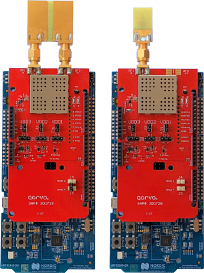
\includegraphics[width=0.2\textwidth]{images/QM33120WDK1_PDP_v2.png}
    \caption{QM33120WDK1 Ultra-Wideband (UWB) Transceiver Development Kit. The Nordic nRF52840DKs (the blue boards behind), are the actual companion boards on which the firmware runs.}
    \label{SEN:fig:eval_kit}
\end{figure}

As already underlined, for the target position estimate, we have used the Ultra-Wideband (UWB) Transceiver Development Kit produced by Qorvo \autoref{SEN:fig:eval_kit}, for which we refer to the official website page\cite{UWBQorvo} for details and datasheet\cite{UWBDatasheet}. For this kit, is also available a firmware that can be requested from Qorvo. Reading the code, we have deduced the following main information:
\begin{itemize}
    \item AoA and distance, are fed directly to the serial port in an encoded string with other quantity like PDoA, status and block number;
    \item The firmware can run in different configurations, depending on the antenna type and the selected communication channel\footnote{The channel type, allows to change between the two supported IEEE standards: IEEE Std. 802.15.4™‐2020\cite{IEEEstd_4} and IEEE Std. 802.15.4z™‐2020\cite{IEEEstd_4z}}: \textit{Jolie} and \textit{Monalisa} are the two antenna types. The possible channels are instead $9$ and $5$. It follows that the antenna can be configured in $4$ different ways, using the parameter \texttt{ANTENNA}: \texttt{JOLIE9}, \texttt{JOLIE5}, \texttt{MONALISA9}, \texttt{MONALISA5}. Our antenna is a \textit{Jolie} and the default channel is $9$, meaning that the \texttt{ANTENNA} parameter is equal to \texttt{JOLIE9} by default. 
    \item PDoA raw measures, are adjusted by means of a stepped linear regression. The steps of this linear regression are defined by a pair of look up table (different for each channel and antenna type): one for the PDoA intervals, and one for the slopes that the liner regression model has to have inside these intervals. All the values were clearly calculated after laboratory test, aiming to reduce the non linear effects present in the raw PDoA measure; 
    \item The PDoA value truly used to calculate AoA by means of the relation \eqref{PRFOR:eq:aoa-pdod}, is the average of the last \texttt{PAVRG} values, corrected with \texttt{PDOAOFF}. \texttt{PAVRG} and \texttt{PDOAOFF} are user definable constant by default equal to $10$ and $0$ respectively. The first defines the values over which perform the moving average: an high value can mitigate the high frequency error, but can worst the sensor performance in detecting PDoA change; on the other side a lower value can detect even rapid changes in the actual PDoA, but the high frequency error contribution is not lowered. \texttt{PDOAOFF} defines instead the offset to apply at the average result as a user calibration.
\end{itemize}

\begin{figure}
    \centering
    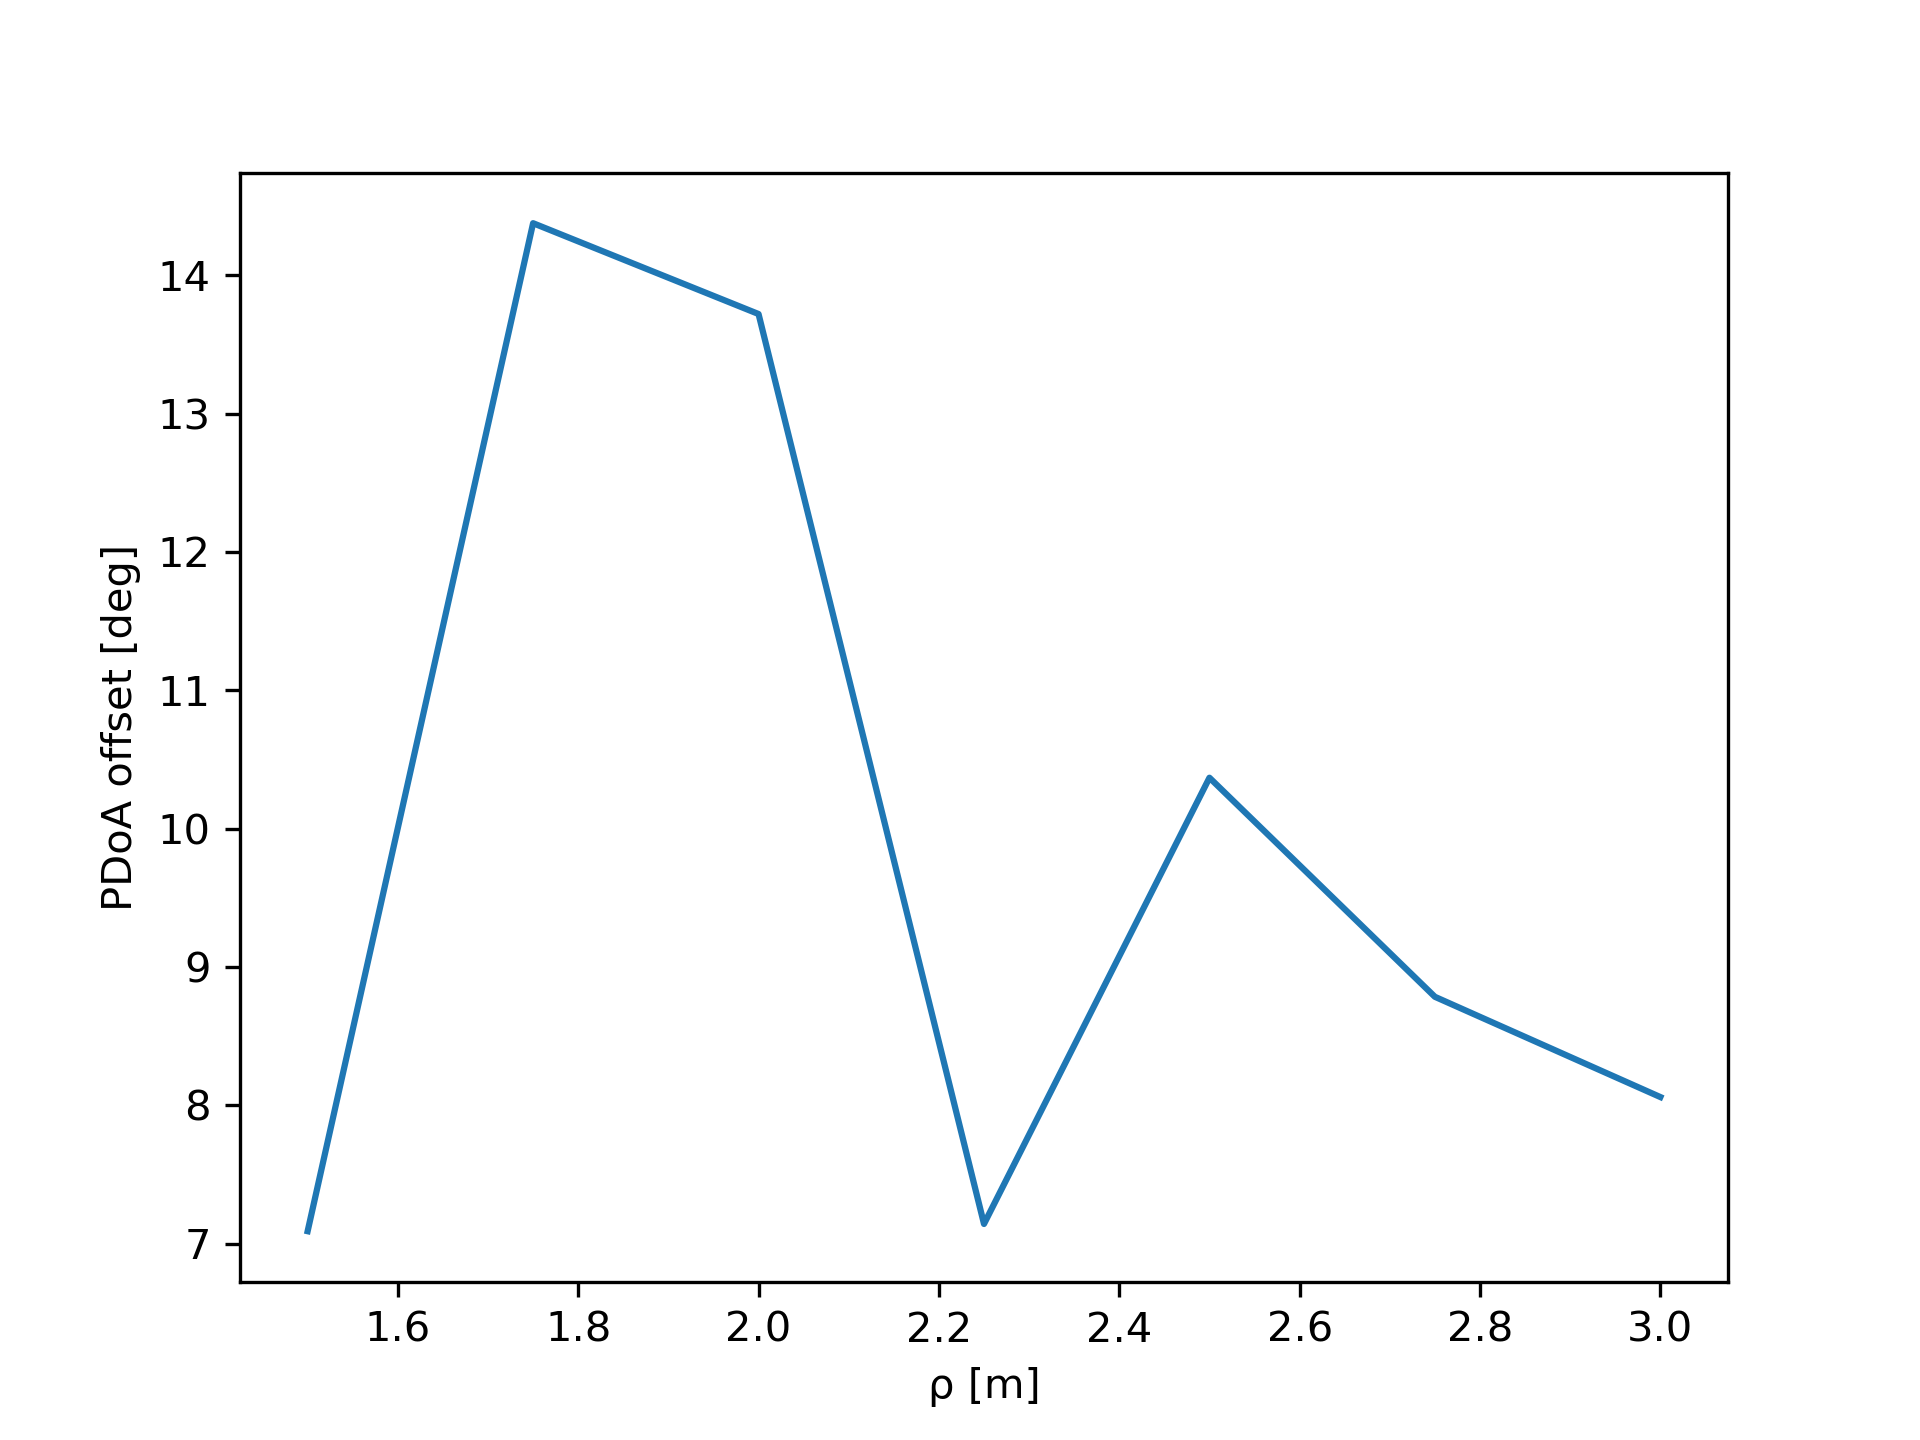
\includegraphics[width=0.45\textwidth]{images/PDOAOFF_trend.png}
    \caption{\texttt{PDOAOFF} at various distances.}
    \label{UWB:fig:PDOAFF}
\end{figure}

\subsection{Characterization}
In order to understand the behavior of the above kit, we have performed a sensor characterization to asses what follows:
\begin{itemize}
    \item Performance difference using the two supported IEEE standards (i.e. channel $9$ or $5$), comparing the results at different angles and distances;
    \item Performance at different tag heights and angles;
    \item Result obtained, by putting the tag behind the double-UWB anchor;
\end{itemize}
Since the first tested channel configuration was the default one (i.e. $9$), the last two results were extracted only for this configuration. By the way, channel type should not change noticeably the validity of the extracted information (e.g. if the kit performance are worsen by a tag height change, the channel should not be a discriminant).\\
All the listed assessment, where performed using MoCap as ground truth and even for precise positioning (i.e. to place the tag at precise distances, angles and eventually heights w.r.t the double UWB).\\

\begin{figure*}
    \centering
    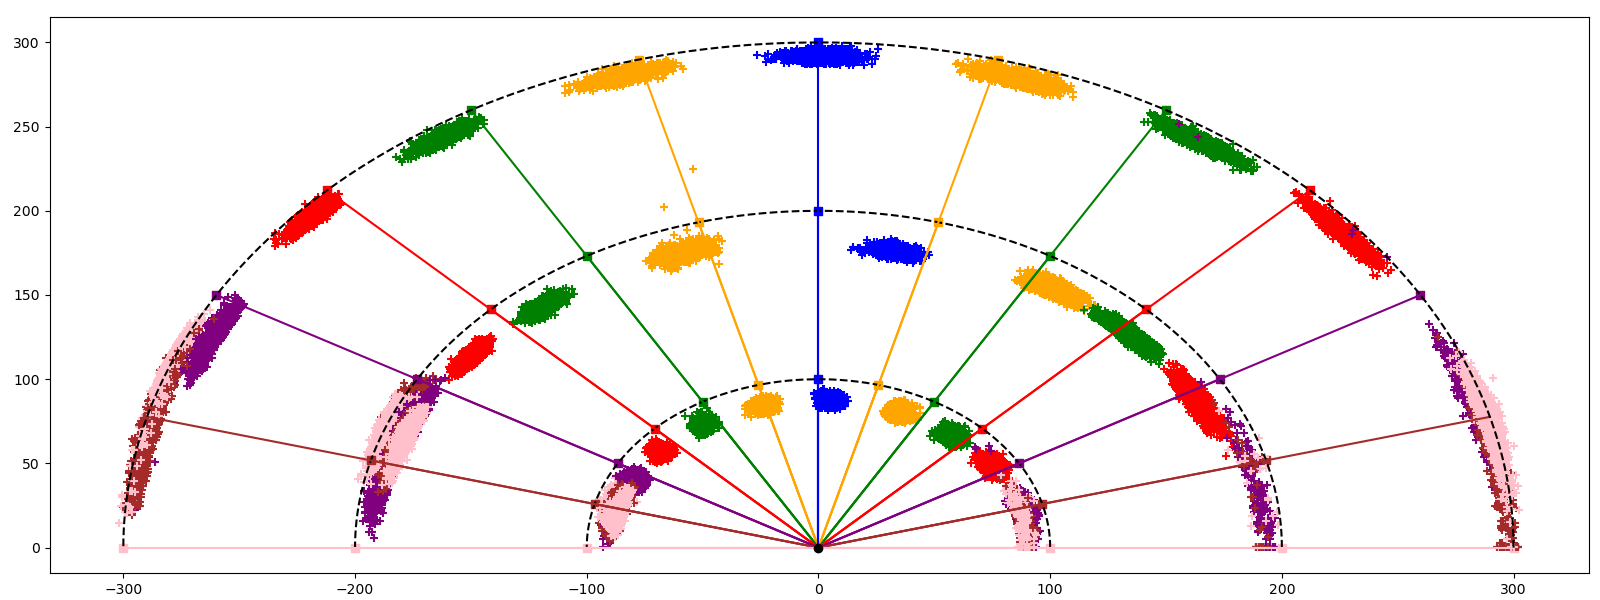
\includegraphics[width=1.0\textwidth]{images/ch9_characterization.png}
    \caption{Location test conducted with channel 9 standards, expressed in centimeters.}
    \label{UWB:fig:ch9test}
\end{figure*}

\begin{figure}
    \centering
    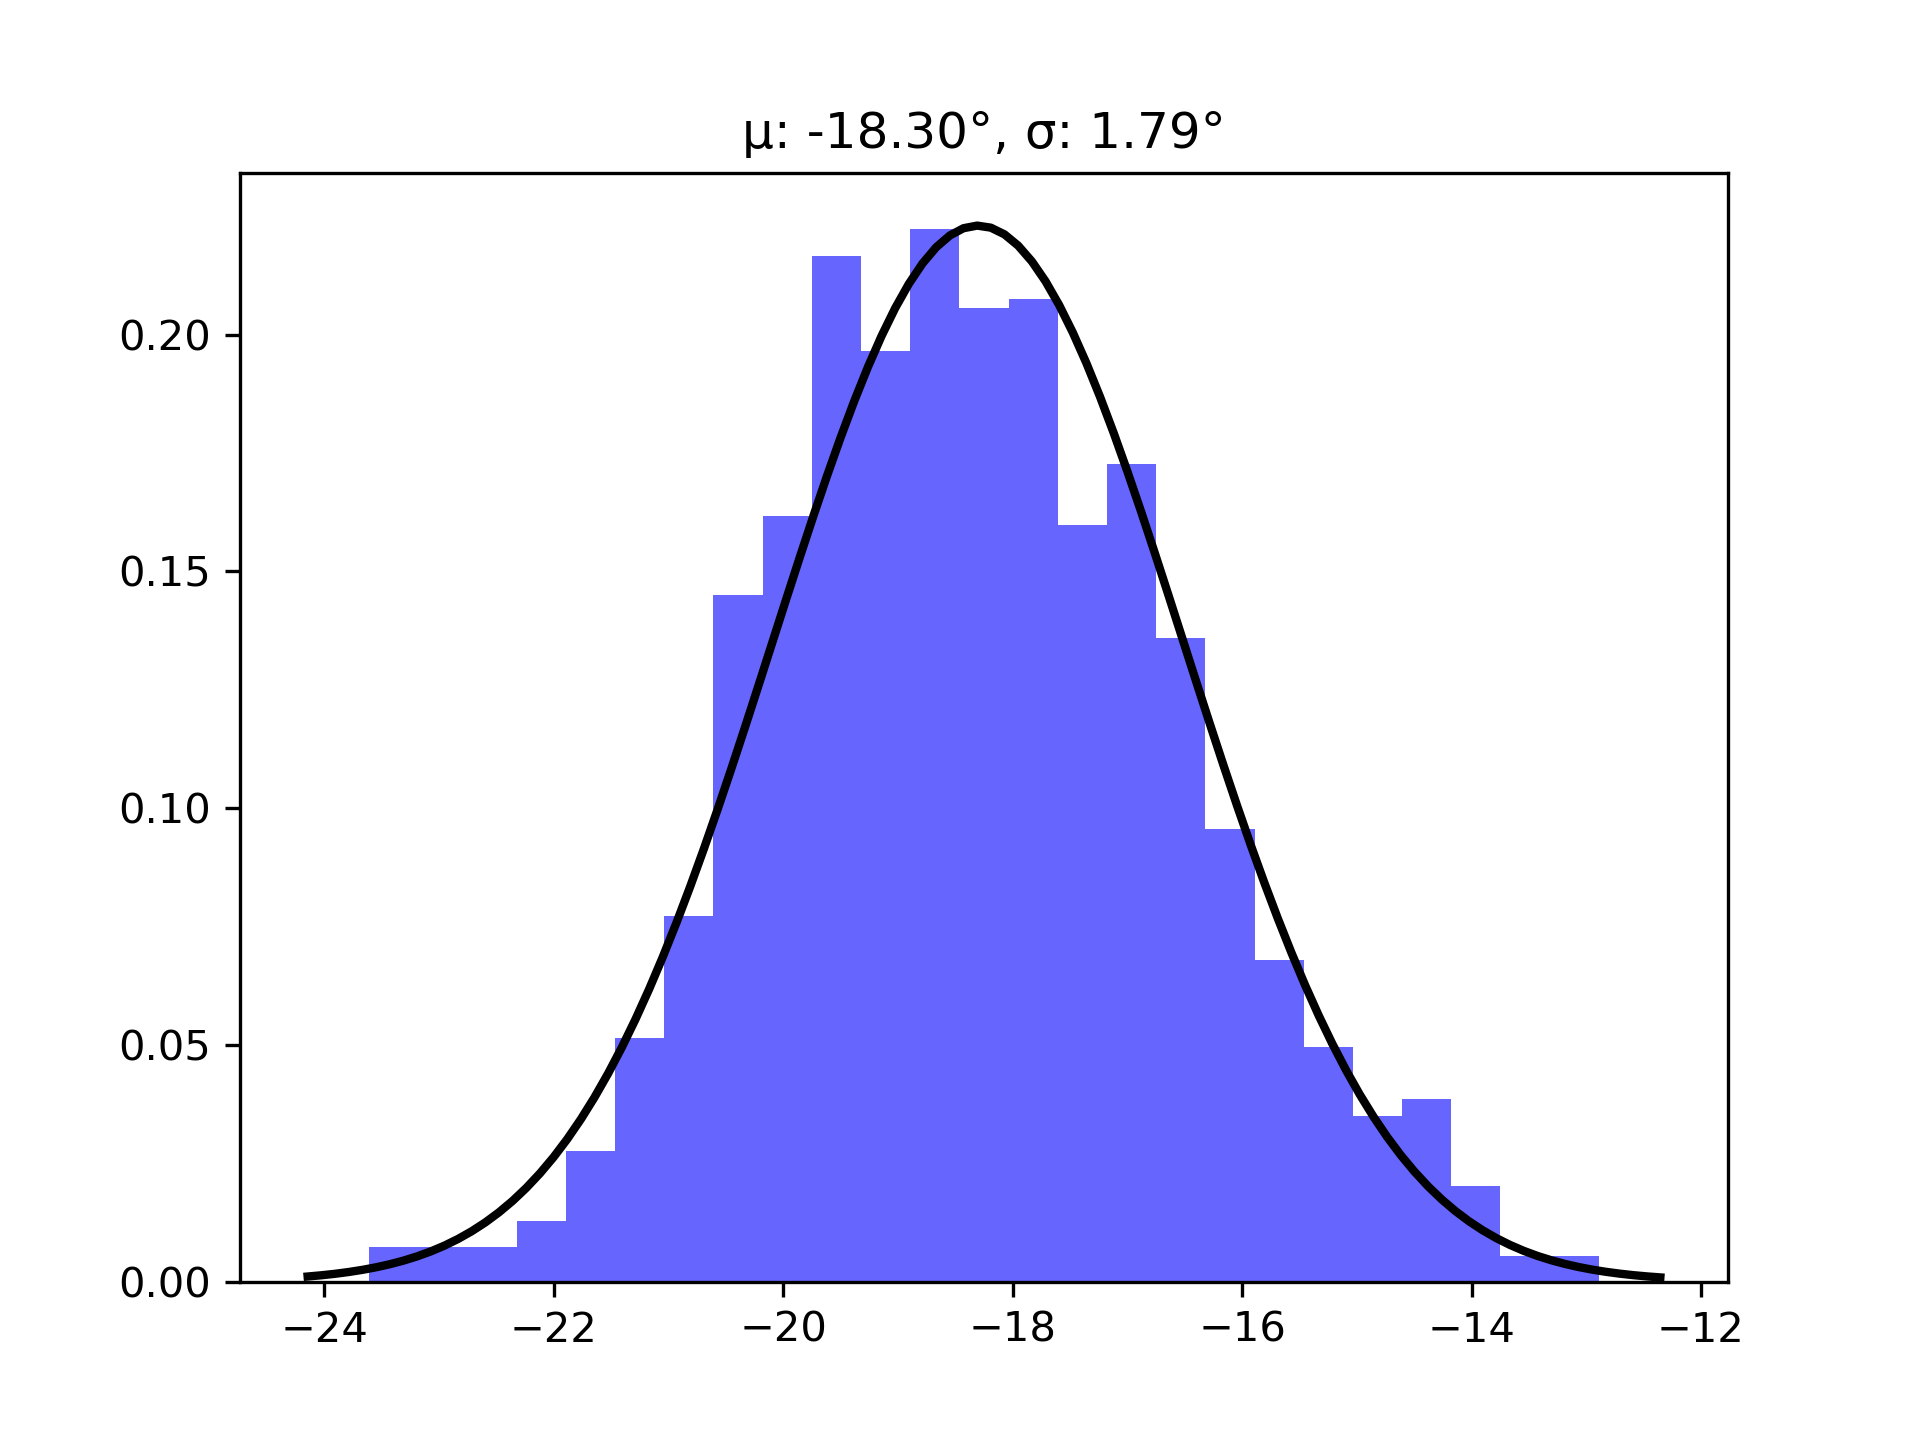
\includegraphics[width=0.45\textwidth]{images/ch9_aoa_hist.png}
    \caption{Channel 9 AoA measurements distribution at $-15$ degrees and $200$ centimeters.}
    \label{UWB:fig:AoA_ch9}
\end{figure}

Since the UWB kit declared working region is the half-plane in front of the double UWB, to compare the behaviour under the two different IEEE standards, we have perform tests in this region, at different discrete values of range and angles. Since that half-plane can be defined with a polar coordinate pair, with undefined radius and angles from $-90$ to $+90$ degree (being $0$ degree when the the tag is in front of the double), we have perform the test as follow:
\begin{itemize}
    \item For channel $9$, at three different range $\rho_9=\begin{bmatrix} 1,2,3 \end{bmatrix} [m]$, and angles from $-90$ to $+ 90$ with a step of $15 deg$;
    \item For channel $5$, at two different range $\rho_5=\begin{bmatrix} 1.5, 2.5 \end{bmatrix} [m]$ and angles from $-90$ to $+90$ for the first range and from $-60$ to $+60$ for the second, again with a step of $15 deg$
\end{itemize}

As suggested by the manufacturer, before the data collection we calibrated the PDoA offset placing the modules at a distance of at least 1.5 meters at 0 degrees, collecting 1000 measures of the PDoA, that ideally should be 0, and averaging the values to obtain the \texttt{PDOAOFF} value to set. For the channel 9 configuration, we determined it at a distance of $2.5$ meters, thinking that the range did not have much influence. However, before the channel 5 data collection, we realized that it changes with the distance, as can be seen in \autoref{UWB:fig:PDOAFF}. Hence, to setup the modules to be used at a distance congruent to the one of the following task, we identified and set the \texttt{PDOAOFF} at 1.5 meters.\\

\begin{figure}
    \centering
    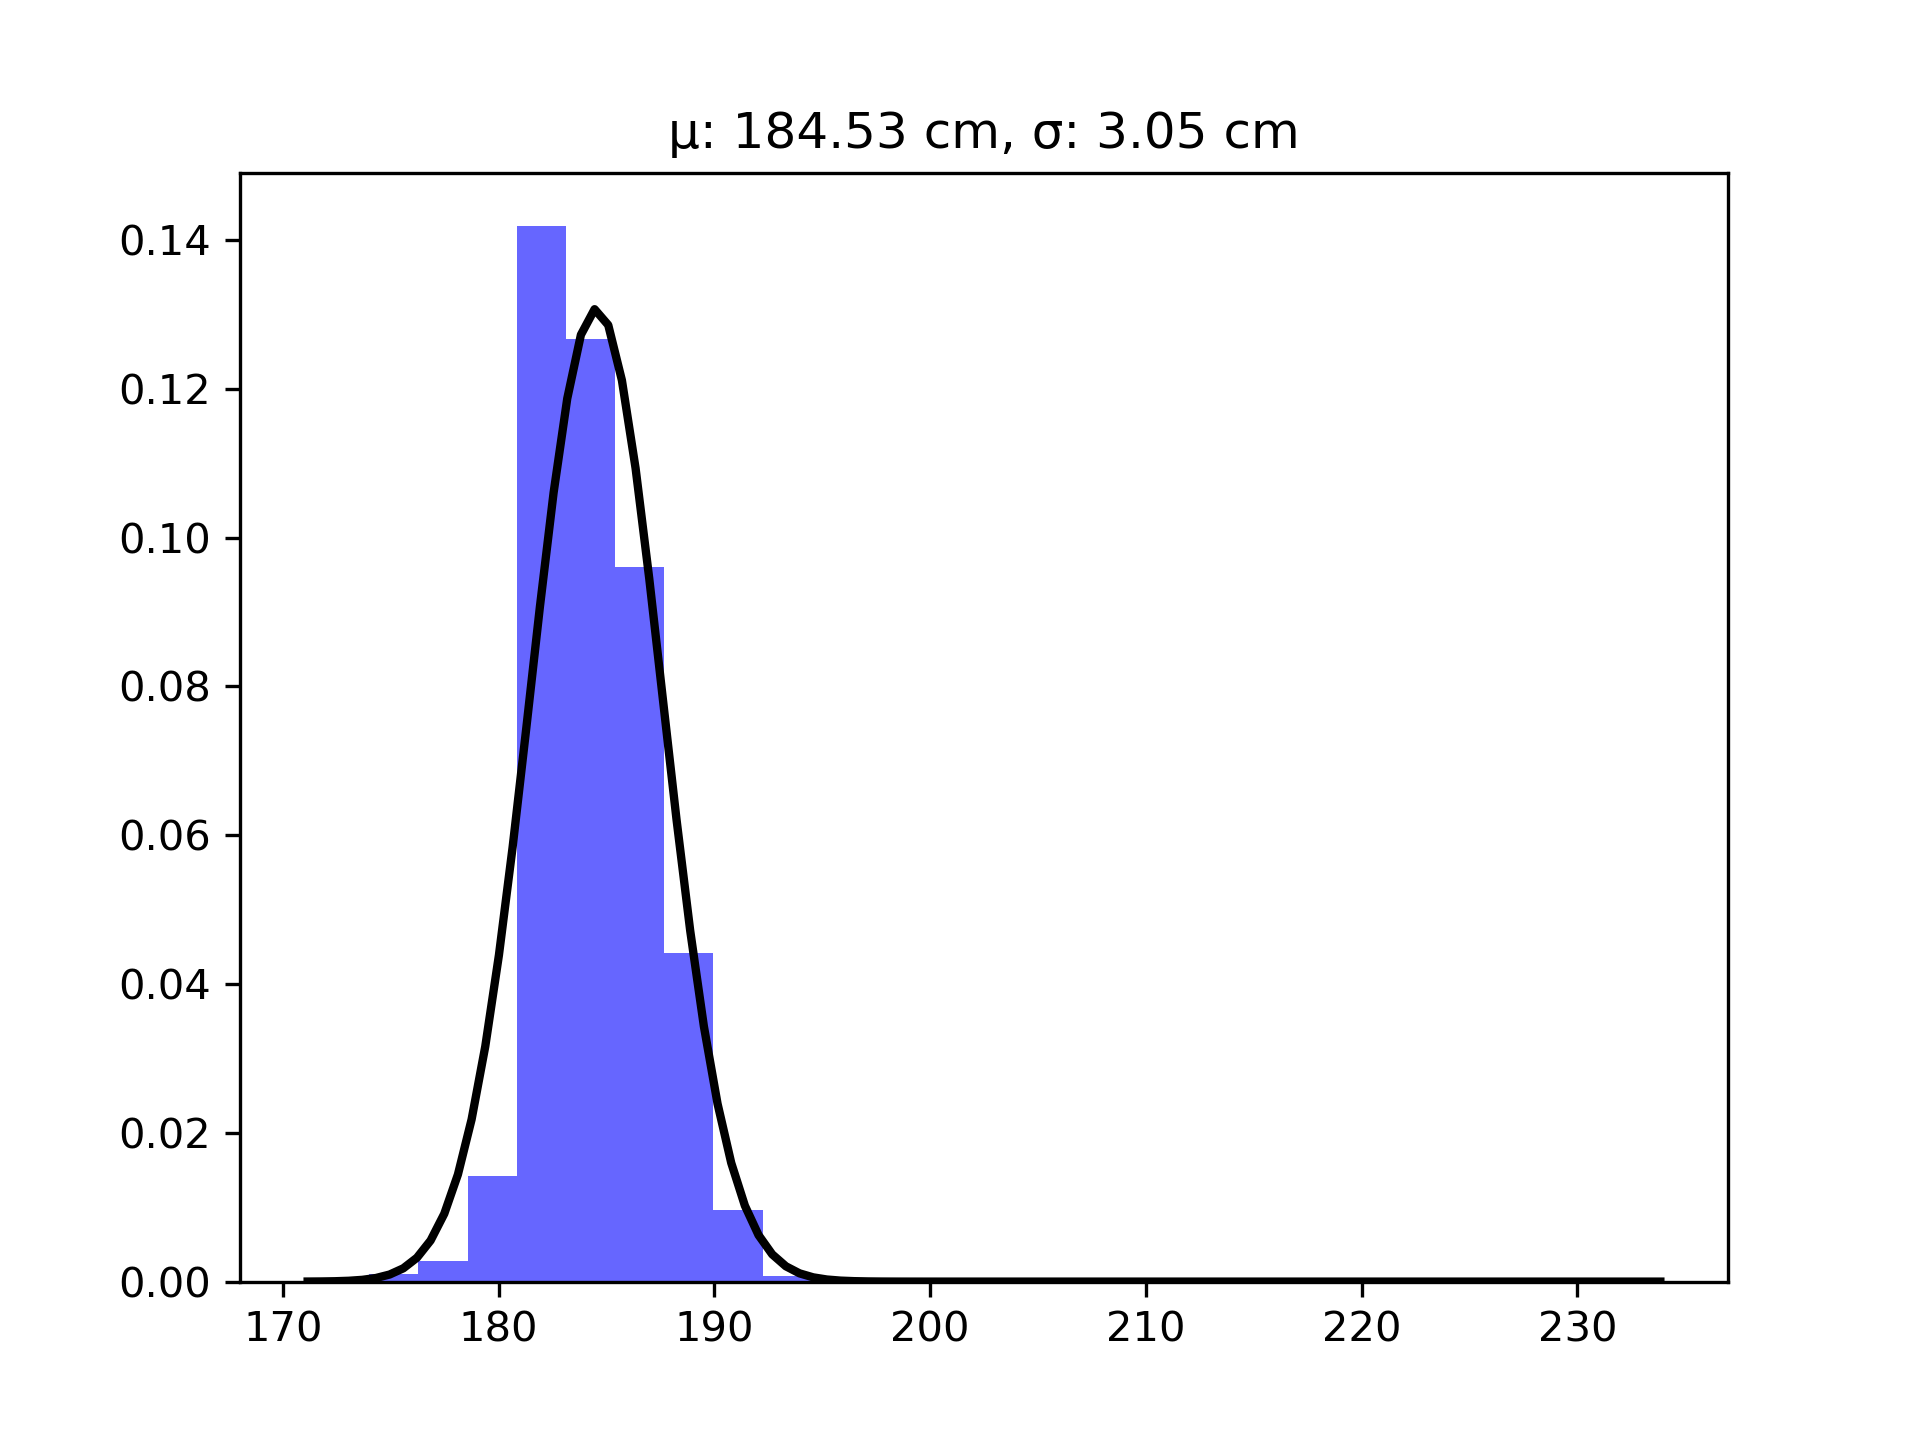
\includegraphics[width=0.45\textwidth]{images/ch9_range_hist.png}
    \caption{Channel 9 range measurements distribution at $-15$ degrees and $200$ centimeters}
    \label{UWB:fig:Range_ch9}
\end{figure}

\begin{figure*}
    \centering
    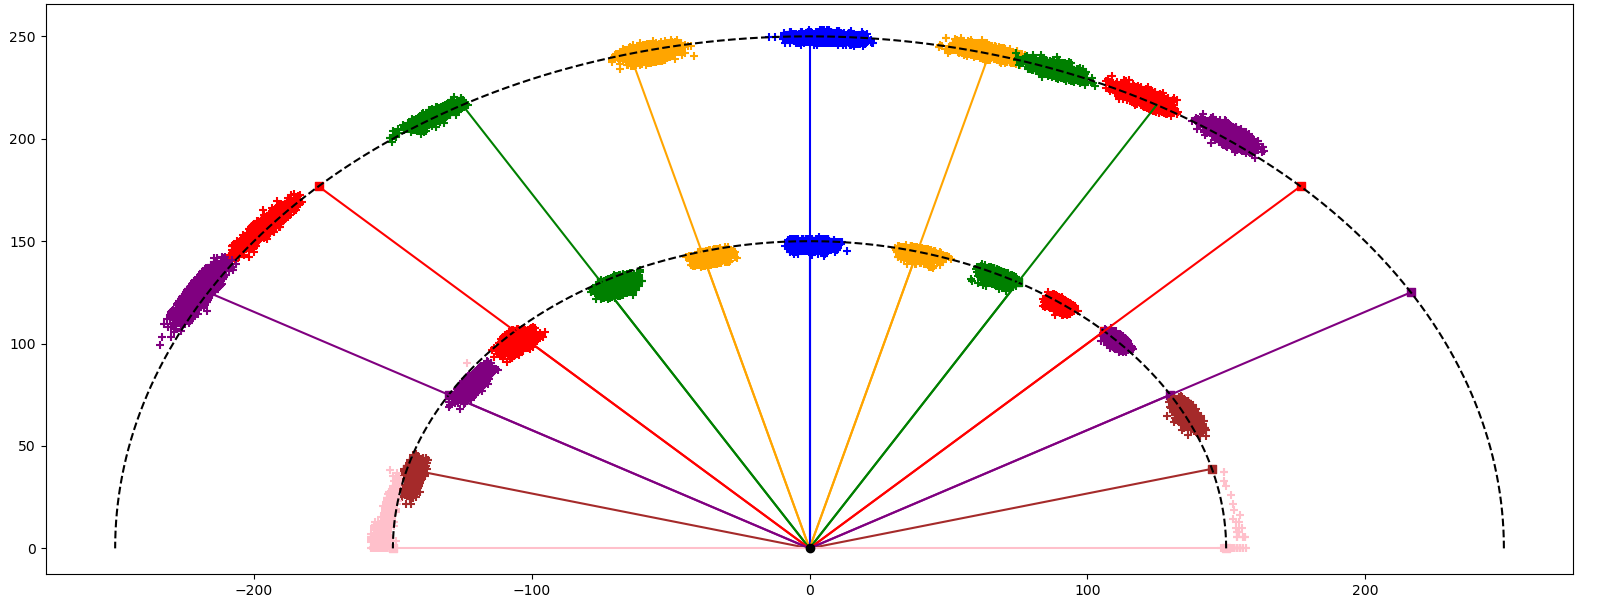
\includegraphics[width=1.0\textwidth]{images/ch5_characterization.png}
    \caption{Location test conducted with channel 5 standards, expressed in centimeters.}
    \label{UWB:fig:ch5test}
\end{figure*}

\begin{figure}
    \centering
    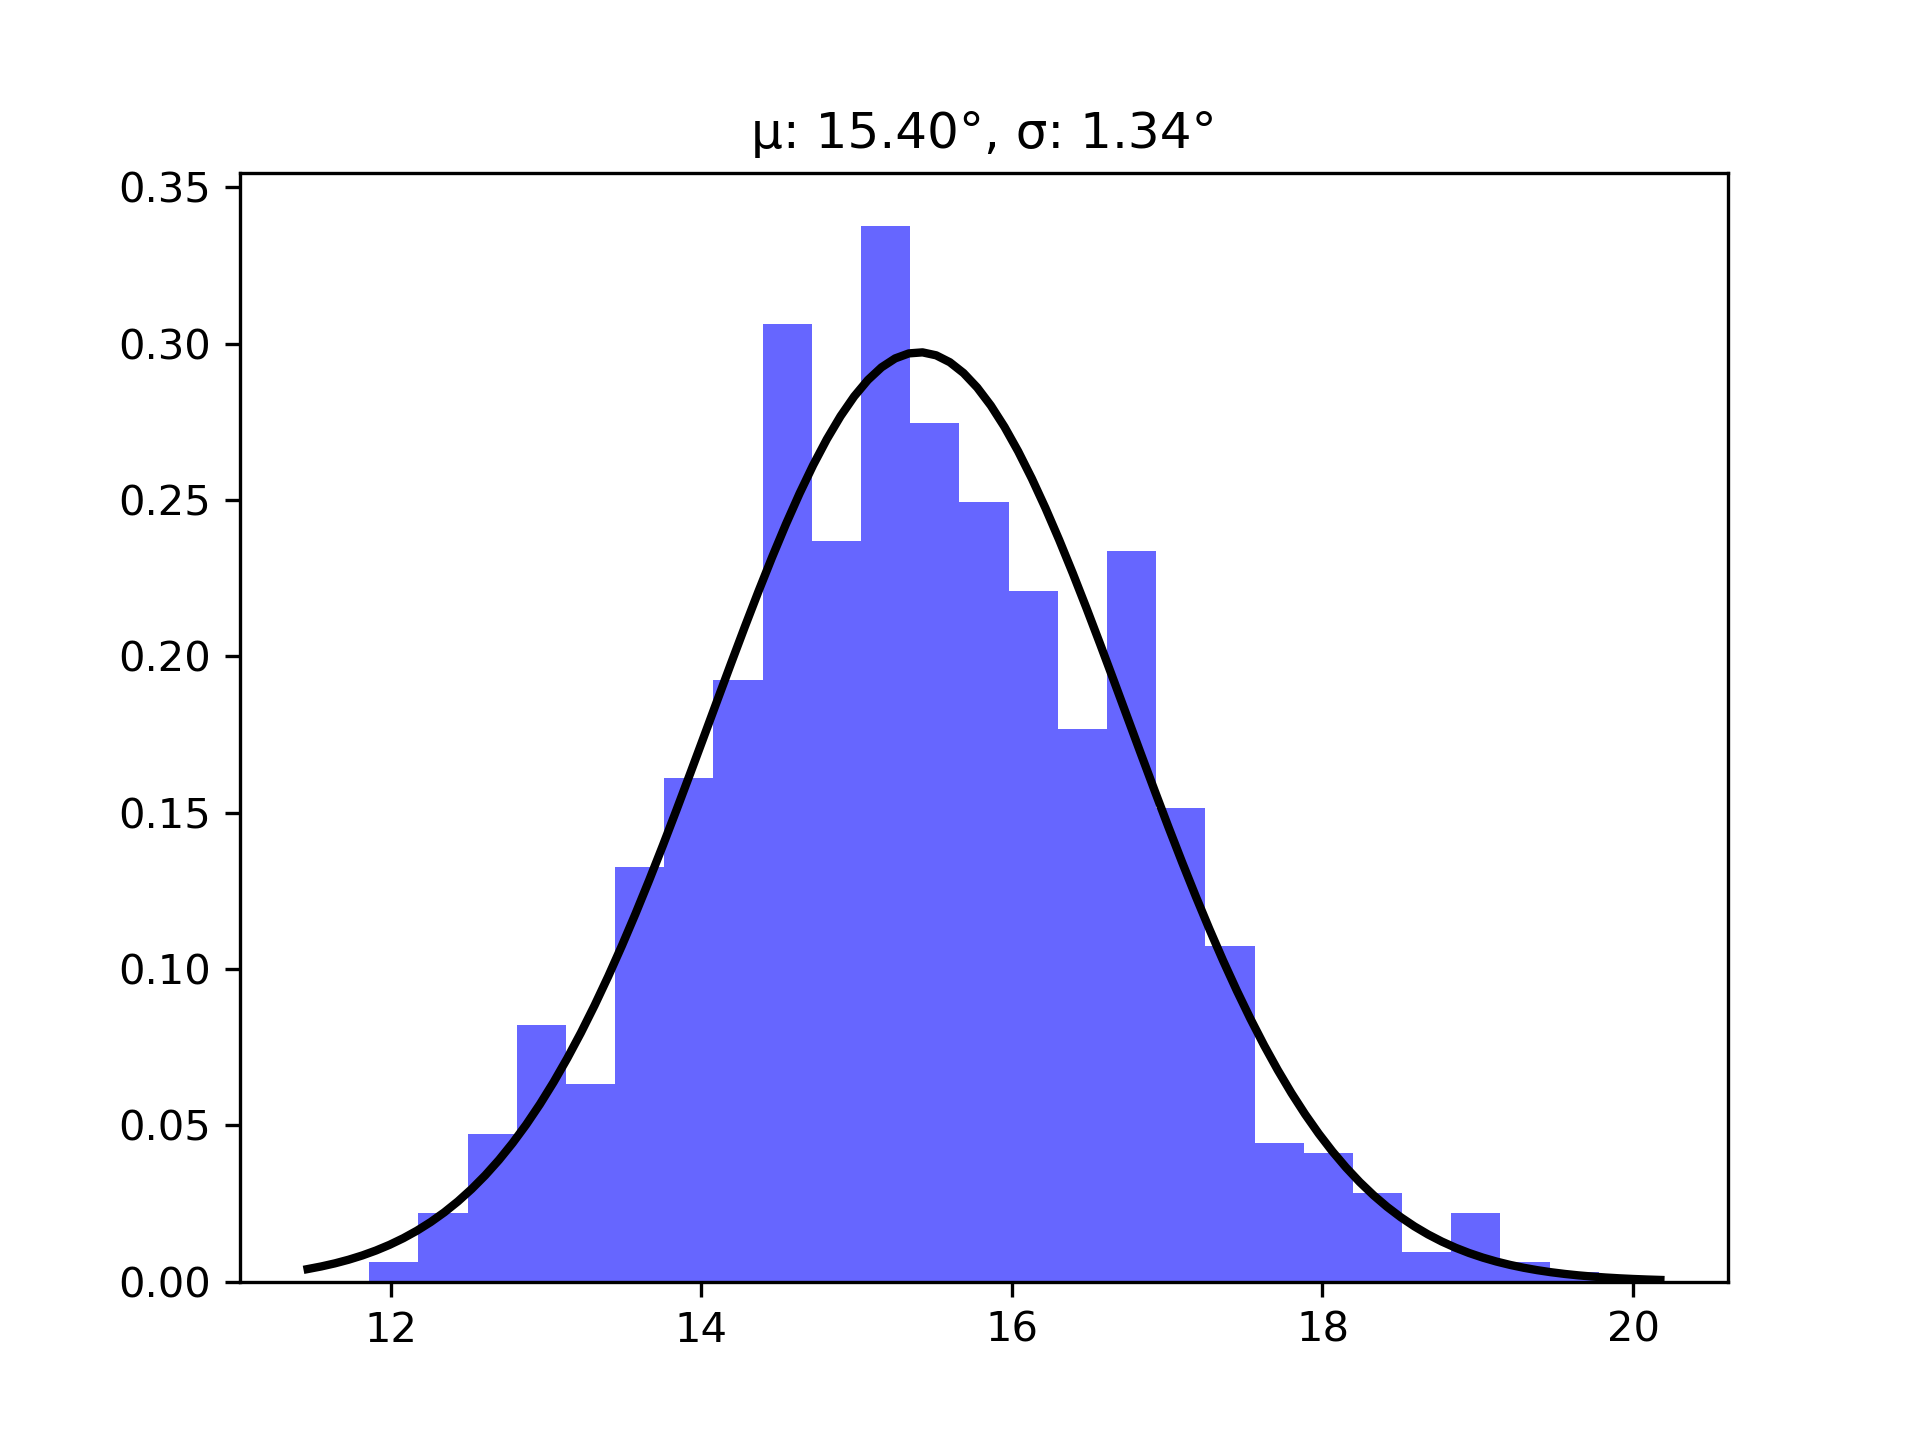
\includegraphics[width=0.45\textwidth]{images/ch5_aoa_hist.png}
    \caption{Channel 5 AoA measurements distribution at $+15$ degrees and $200$ centimeters.}
    \label{UWB:fig:AoA_ch5}
\end{figure}

\paragraph{Channel Comparison}
The tests results for channel 9, are depicted in \autoref{UWB:fig:ch9test}. The graph shows different behaviours at different distances. For example at a distance of $3$ meters the estimated angle is quite good, whereas at $2$ meters it shows different behaviours for the negative and the positive part of the half-plane. Indeed for positive angles it shows better values. Despite this, the measured angles are generally bad. This behaviour could be caused by the great variation of \texttt{PDOAFF} at $2$ meters w.r.t. $2.5$, as shown in \autoref{UWB:fig:PDOAFF}. At $1$ meter the results are slightly better, but still there is asymmetry between positive and negative part. Another characteristic  to denote, is that despite the distance, at angles greater then $75$ degree (and $-75$), the angles are not reliable and tend to be much more scattered. For what concerns the range, a not constant negative bias is always present. The data clouds, shows instead an almost constant spread, indicating that the standard deviation of both range and angles, are constants. A pair of distribution examples, are presented in \autoref{UWB:fig:AoA_ch9}, \ref{UWB:fig:Range_ch9}. Both shows a bias w.r.t. the actual angle and range, but their distributions are gaussian-like, with $\sigma_{\alpha} = 1.79$ ° and $\sigma_{\rho} = 3.05$ cm and mean error of $3.30$ ° for the angle and of $15.47$ cm for the range. Comparing these values with the specifications of the manufacturer, reported in \autoref{UWB:tab:sensorspec}, is possible to see that the standard deviation is in accordance with the declared one both for the angle and the range. For what concerns the accuracy, the angle is inside the accuracy interval declared while it is not the case for the range. However, as can be seen in \autoref{UWB:fig:ch9test}, if instead of the measurement at $2$ meters and $-15$ degrees one would consider the data at the same distance and angle mirrored, the angle would not be anymore in the accuracy interval.\\

\begin{table}
    \centering
    \begin{tabular}{ | m{1.3cm} | m{1.2cm}| m{2.1cm} | m{0.7cm} |} 
        \hline
        &  accuracy & standard deviation & Units\\ 
        \hline
        Range & $\pm $ 6 & 3 & cm\\ 
        \hline
        AoA CH9 &$\pm$ 6.25 & 2.5 & deg \\
        \hline
        AoA CH5 &$\pm$ 6.25 & 2 & deg \\
        \hline
    \end{tabular}
    \captionsetup{type=table}
    \caption{Manufacturer declared Location Accuracy Characteristics. The values are intended after calibration, measured in line of sight in a noise-free environment. See Datasheet p.17 for reference\cite{UWBDatasheet}}
    \label{UWB:tab:sensorspec}
\end{table}
The test for the channel 5, is depicted in \autoref{UWB:fig:ch5test}. As previously specified, this test was conducted by tuning the PDoA offset at a distance congruent with the one of the following task, that is $1.5$ m, in order to reduce all the error in the working region. To this end, even the tested ranges were changed to a pair $1.5$ and $2.5$ m.\\
Also for this test, the asymmetry between negative and positive region is clear. Despite the slightly lower accuracy in range, the left region, shows better performance in angle measurements. Overall the general accuracy is visibly better for this configuration, and more precisely in the cone from $-15$ to $+15$ degrees, the localization is very good. This is an important results, since, as will be later shown, during the simulation the angle measured by the simulated UWB remains almost always inside this region. Two representative distribution for angle \autoref{UWB:fig:AoA_ch5} and range \autoref{UWB:fig:Range_ch5} measurements are presented. their distributions are gaussian-like, with $\sigma_{\alpha} = 1.34$ ° and $\sigma_{\rho} = 1.66$ cm and mean error of $0.4$ ° for the angle and of $0.68$ cm for the range. Comparing this results with the declared specifications for channel 5 \autoref{UWB:tab:sensorspec}, both accuracies and standard deviations are congruent. In particular the accuracy error, both for range and Aoa, is very low.\\
As an overall conclusion, channel 5 outperformed channel 9, making it our choice for the presented application.\\

\begin{figure}
    \centering
    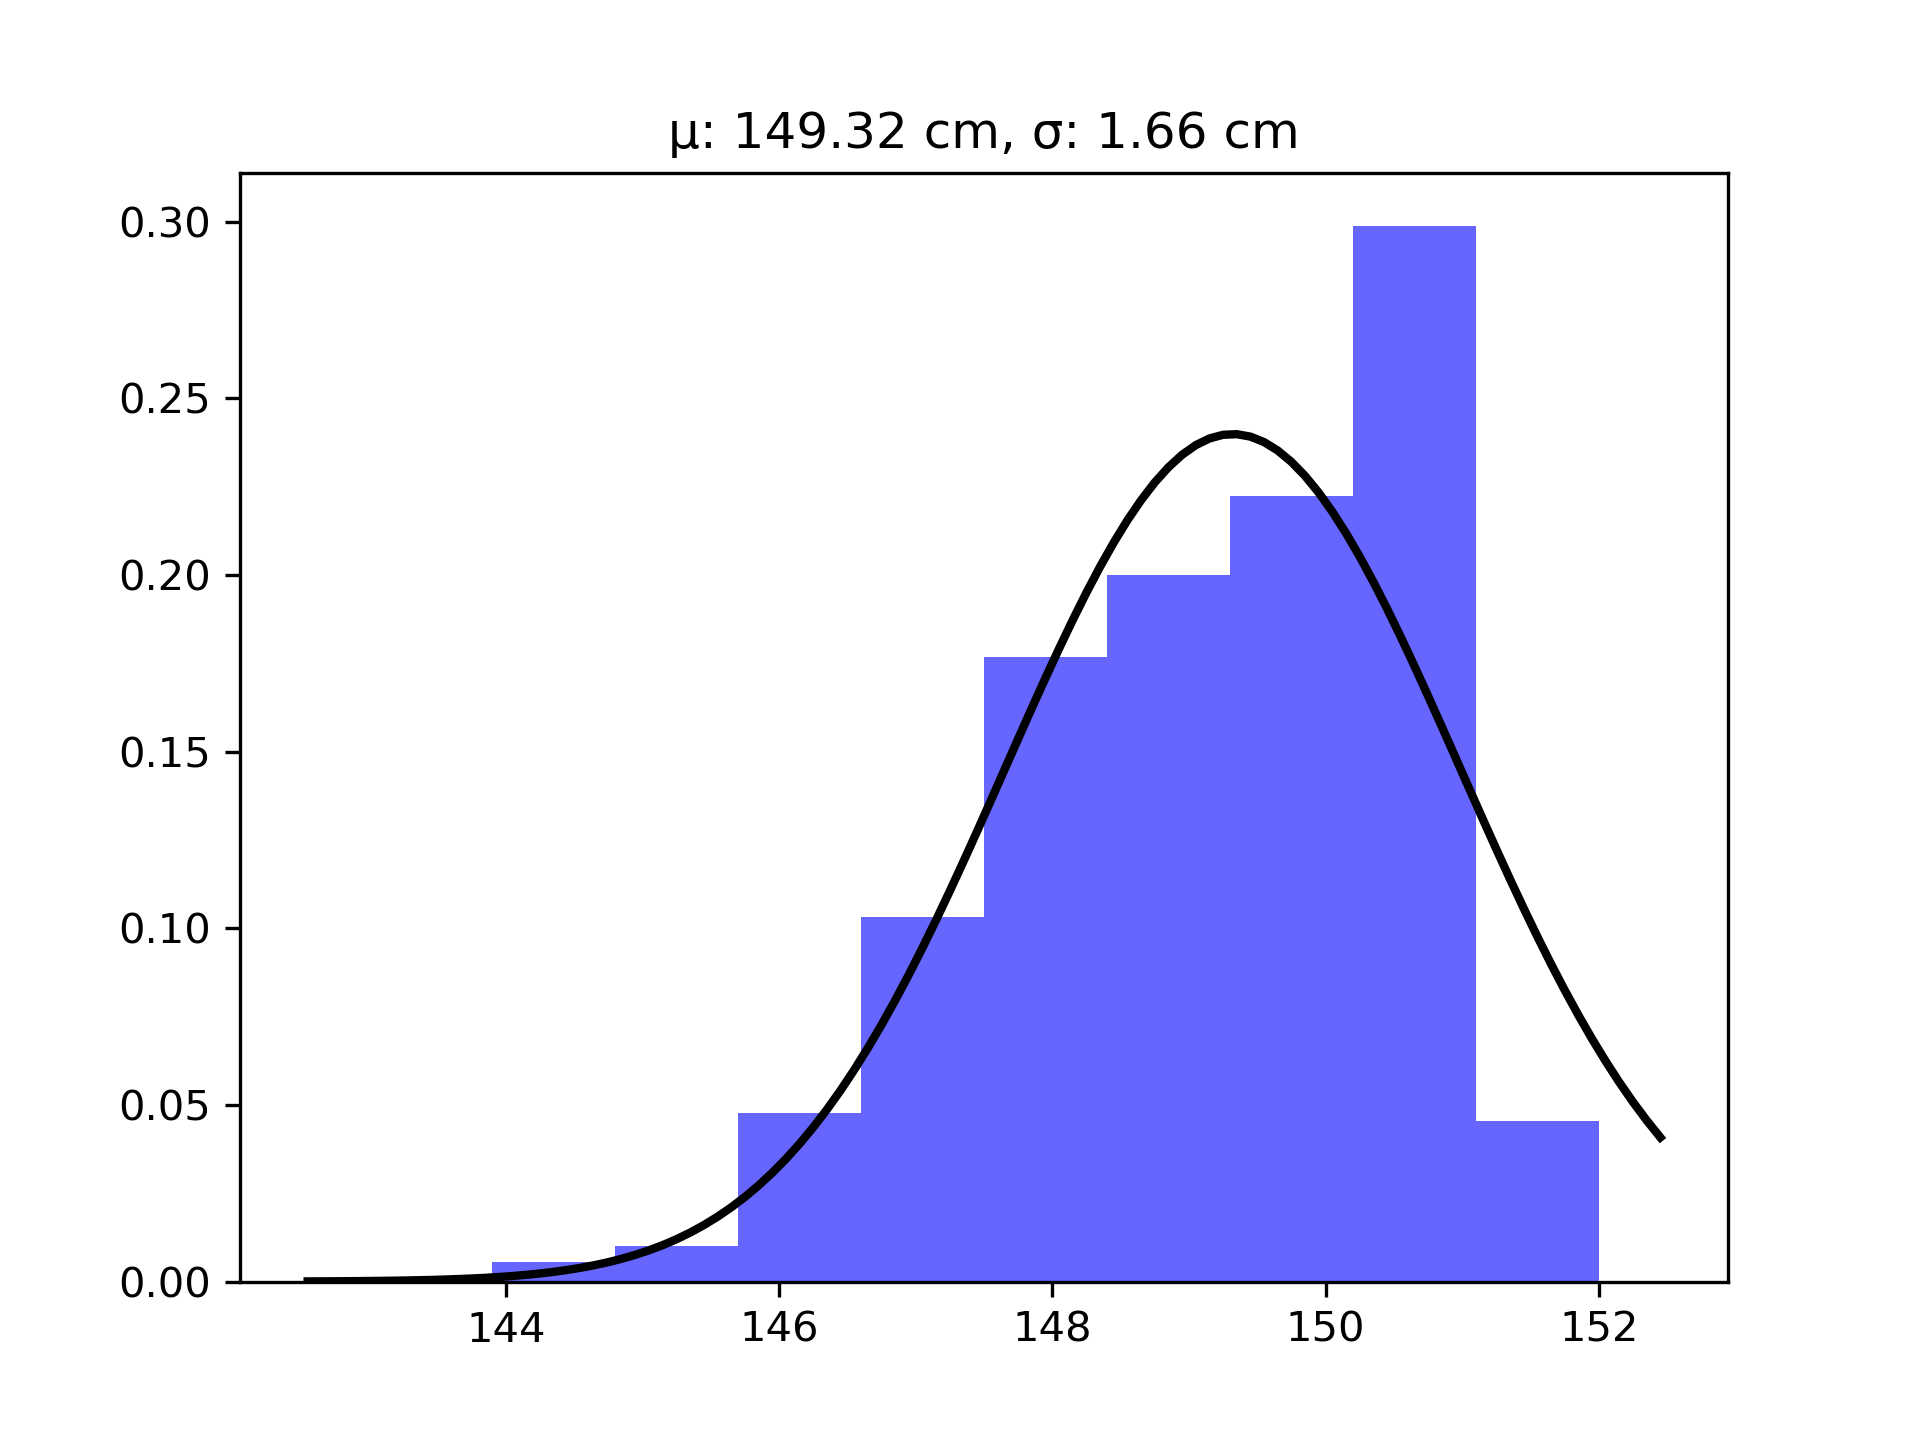
\includegraphics[width=0.45\textwidth]{images/ch5_range_hist.png}
    \caption{Channel 5 range measurements distribution at $+15$ degrees and $200$ centimeters}
    \label{UWB:fig:Range_ch5}
\end{figure}

\paragraph{Performance for height change}
in our Leader-follower application, the angle estimation robustness against the height difference between leader and follower, is an important requirement. Indeed in our application the target is supposed to be a ground robot, so the tag is placed at a low height. To asses the kit performance at different height, we have placed the target antenna at 3 different heights $h=[46,60,115]$ centimeters and at different angles $\alpha = [0,-30,-60,-75]$ degrees. The result are exposed in \autoref{UWB:fig:ch9_heights}. It can be seen that the height difference does not remarkably change the measured angle. Only for the measurements at $-75$ degree the measures are bad but, as previously stated, this is an angle related behaviour, so it does not invalidate this test outcomes.\\

\begin{figure}
    \centering
    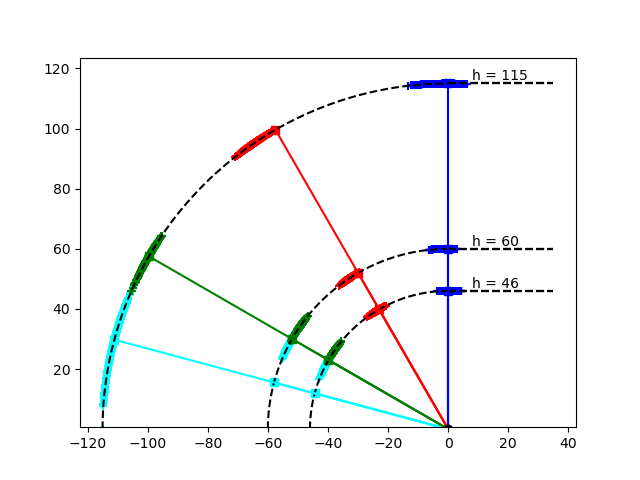
\includegraphics[width=0.48\textwidth]{images/ch9_heights.png}
    \caption{Angle measurements at different heights and at a constant x-y distance of $200$ cm.}
    \label{UWB:fig:ch9_heights}
\end{figure}

\paragraph{Behind the double UWB results}
in order to fully understand the sensor behaviour in different situations, a test with the target antenna behind the the double at a distance of $1$ meter was conducted. The results, together with the equivalent measure at one meter taken in front, are presented in \autoref{UWB:fig:ch9_behind}. As expected, given the manufacturer indication, the measure behind are quite chaotic, and both angles and ranges are mostly wrong. Even the data clouds are spread differently not resembling the constant behaviour seen for the front taken measures.

\begin{figure}
    \centering
    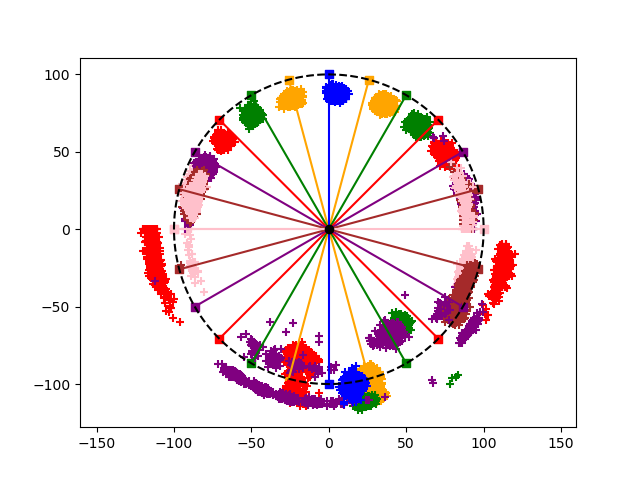
\includegraphics[width=0.48\textwidth]{images/ch9_behind_measure.png}
    \caption{Localization comparison between front and behind taken measures, expressed in centimeters.}
    \label{UWB:fig:ch9_behind}
\end{figure}

\paragraph{Conclusions}\label{UWB:conclus}
This evaluation kit has the potential to became a valid tool in Leader-follower applications, but some extra work on the sensor is needed. The main drawback is that the angle offset is a non linear function of the distance, and for application in which a dynamic range change is involved, this UWB pair is not suitable. To compensate for this behaviour, some work in modeling this offset's non-linearity is suggested. For what concern our purposes, this kit is precise enough, since in the region of interest (i.e. at $1.5$ meters $\pm 15$ degrees), it works pretty well. Even in the case of having wider angle and distances, since localization maintain his sign (e.g. if the true angle is $60$ degree, it measure $45$ not $-45$), our policy tends to converges towards the $0$ degree angle and $1.5$ meters distance, and so even in the presence of large accuracy error, the quadcopter is still somehow able to perform decently. Another modification effect on the measures noticed , that is not presented in this characterization, is the change in localization given by the relative orientation between the antennas. Indeed the best measures are obtained if the tag is placed radially w.r.t. the double, whereas important angle errors can be introduced if this condition is not respected (especially at short distances). This can overall truly impact the localization performance. In the real test, whose results will be later exposed, this last behaviour is surely responsible for a great amount of the localization error.

\section{Results}\label{RESULTS}
\begin{figure}
    \centering
    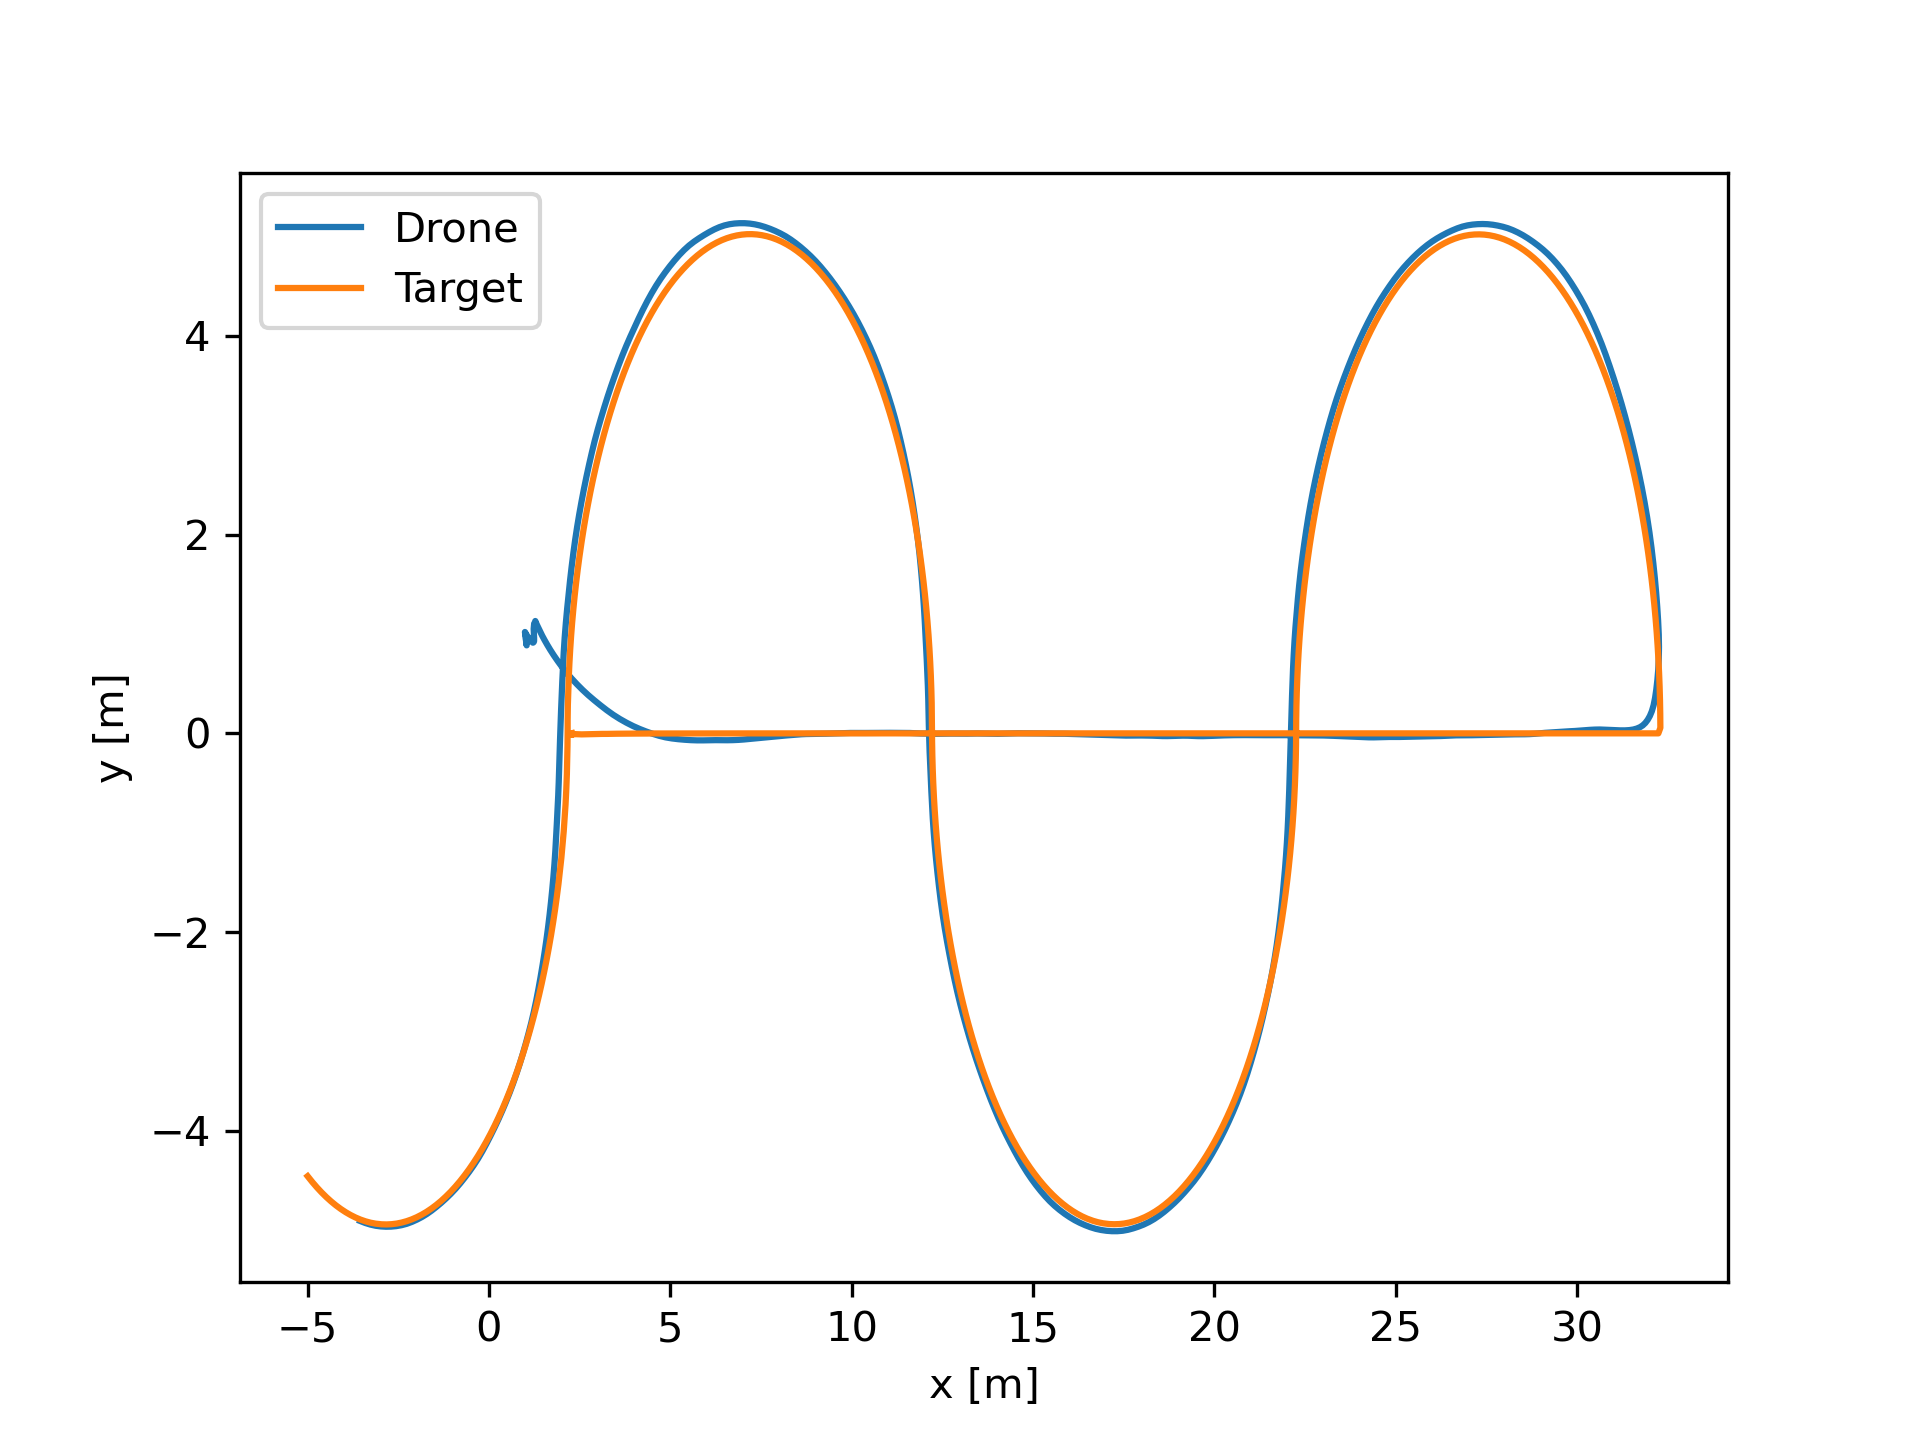
\includegraphics[width=0.48\textwidth]{images/Simulation/Drone_Target x-y Position.png}
    \caption{Target and drone trajectory in simulation.}
    \label{SIM:traj}
\end{figure}

\begin{figure}
    \centering
    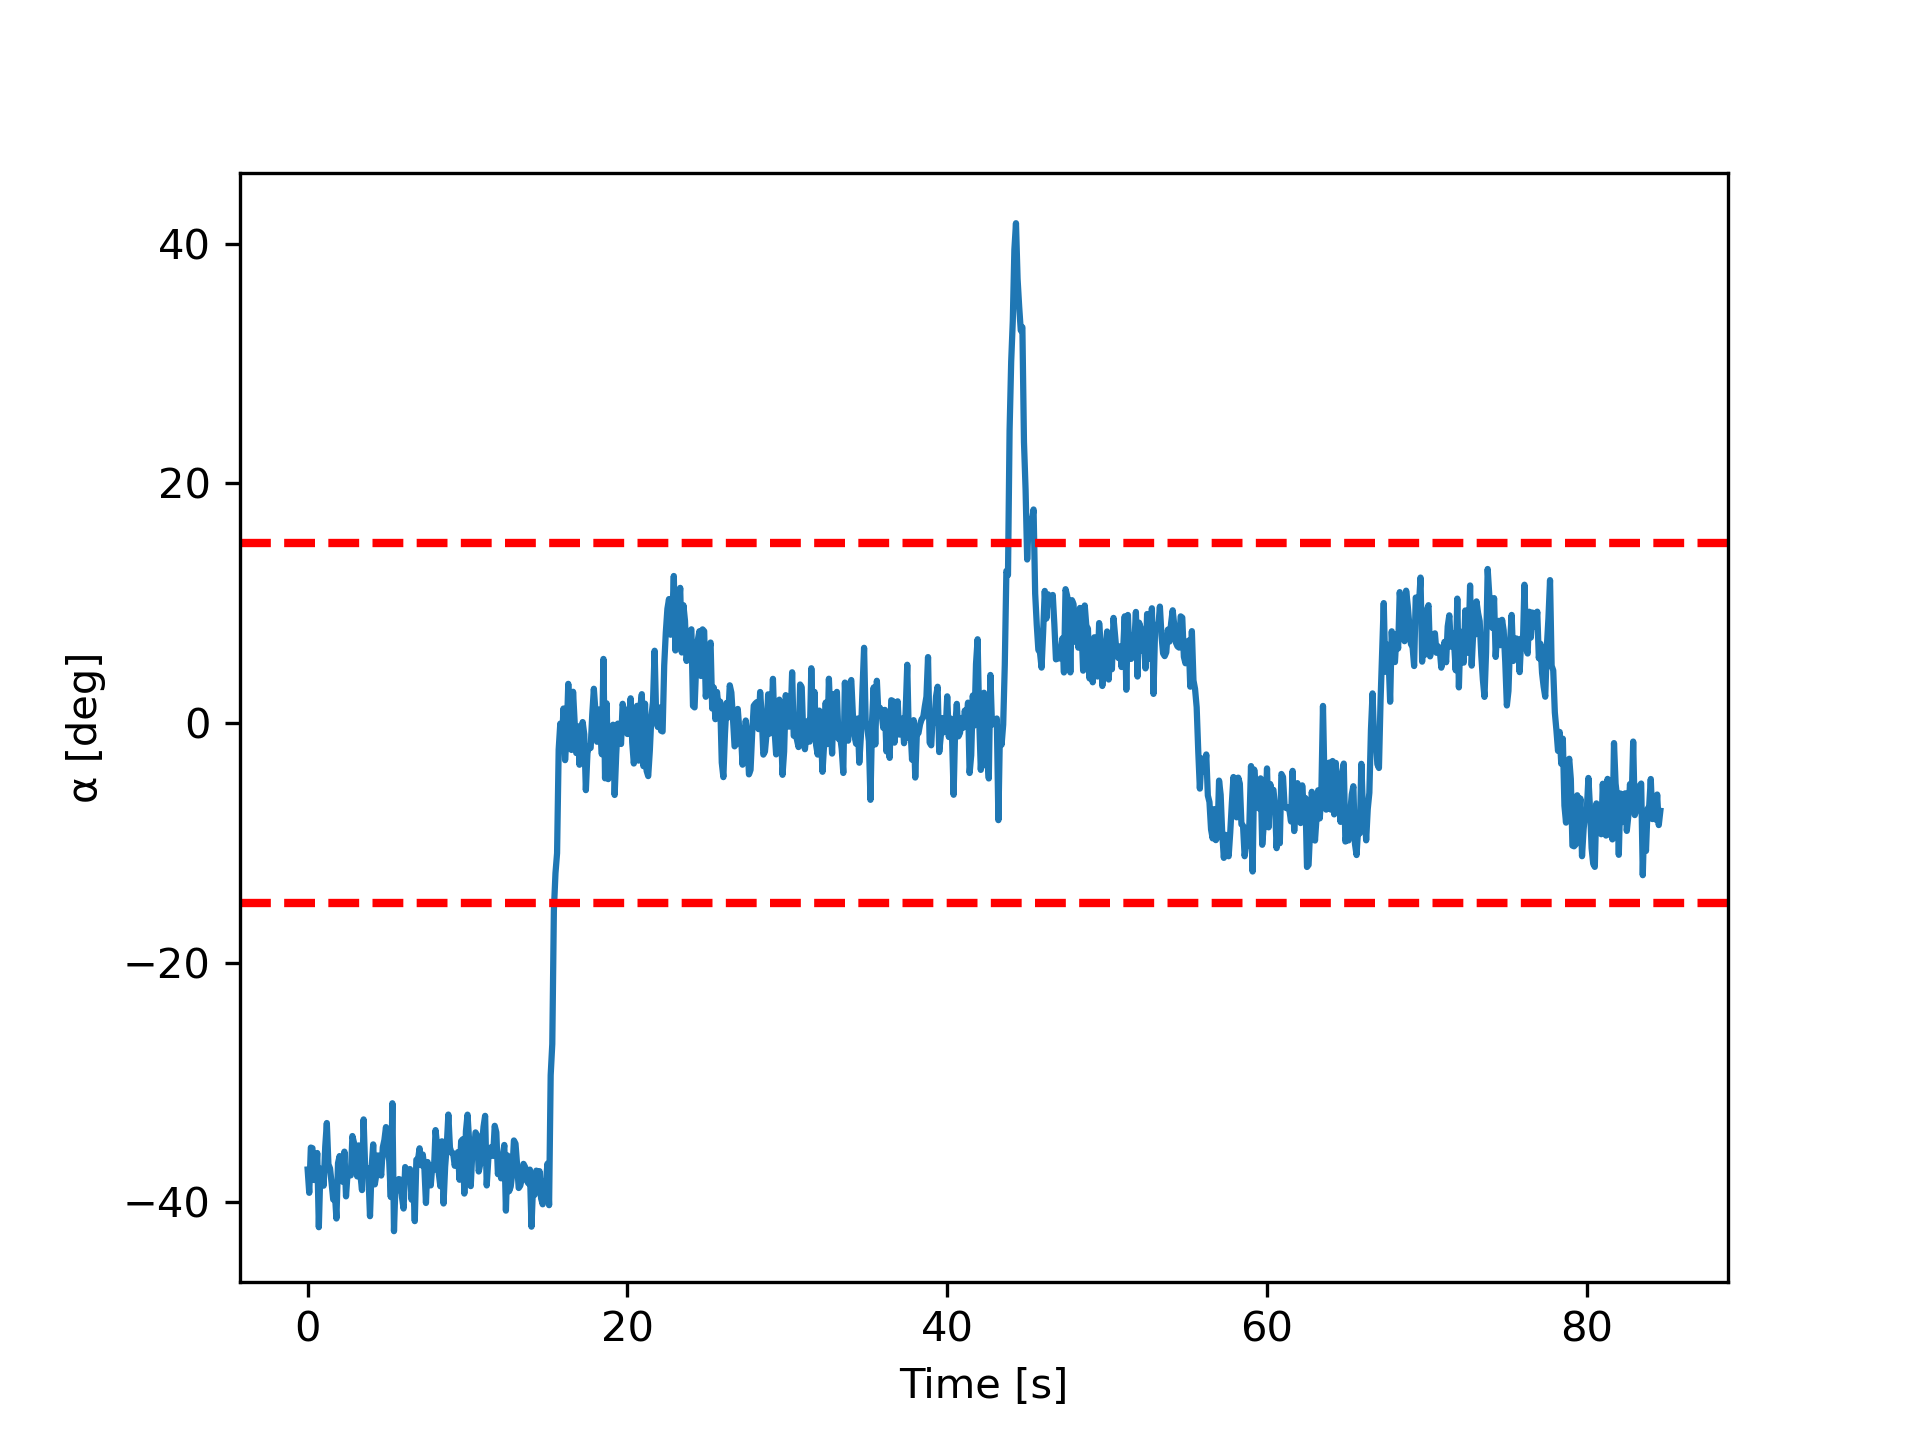
\includegraphics[width=0.48\textwidth]{images/Simulation/AoA measures.png}
    \caption{Measured AoA in simulation. The two red dotted lines, indicates the $\pm$ $15$ deg region in which the kit performs better. The fact that the measured angle remains inside this region, is an important results for the real implementation.}
    \label{SIM:aoa in time}
\end{figure}

\subsection{Simulation}\label{SIM_RES}
To test the validity of the following algorithm in various motion conditions we setup a simulation in which the target moves at a velocity of $5$ km/h in two ways: in a first phase doing a straight line and then changing direction and doing a sine wave trajectory, testing the quadcopter behaviour during curved motion. The noise that affects the simulated range and AoA sensor is white gaussian with zero mean and the standard deviations, in the light of what has emerged during the sensor characterization, are set equals to those declared by the manufacturer, as in \autoref{UWB:tab:sensorspec} for the channel 5. The set following distance is $1.5$ meters and the flight height $2$ meters.\\
In \autoref{SIM:traj} is possible to see in yellow the trajectory of the target that starts at the origin and in blue the movement of the quadcopter. After a first phase in which the drone performs the takeoff while the target starts its motion in the x direction, is possible to see that the quadcopter is able to follow accurately the movements done by the target, even in curve, if the curvature radius is not too small and compatible with the demanded following distance.\\

\begin{figure}
    \centering
    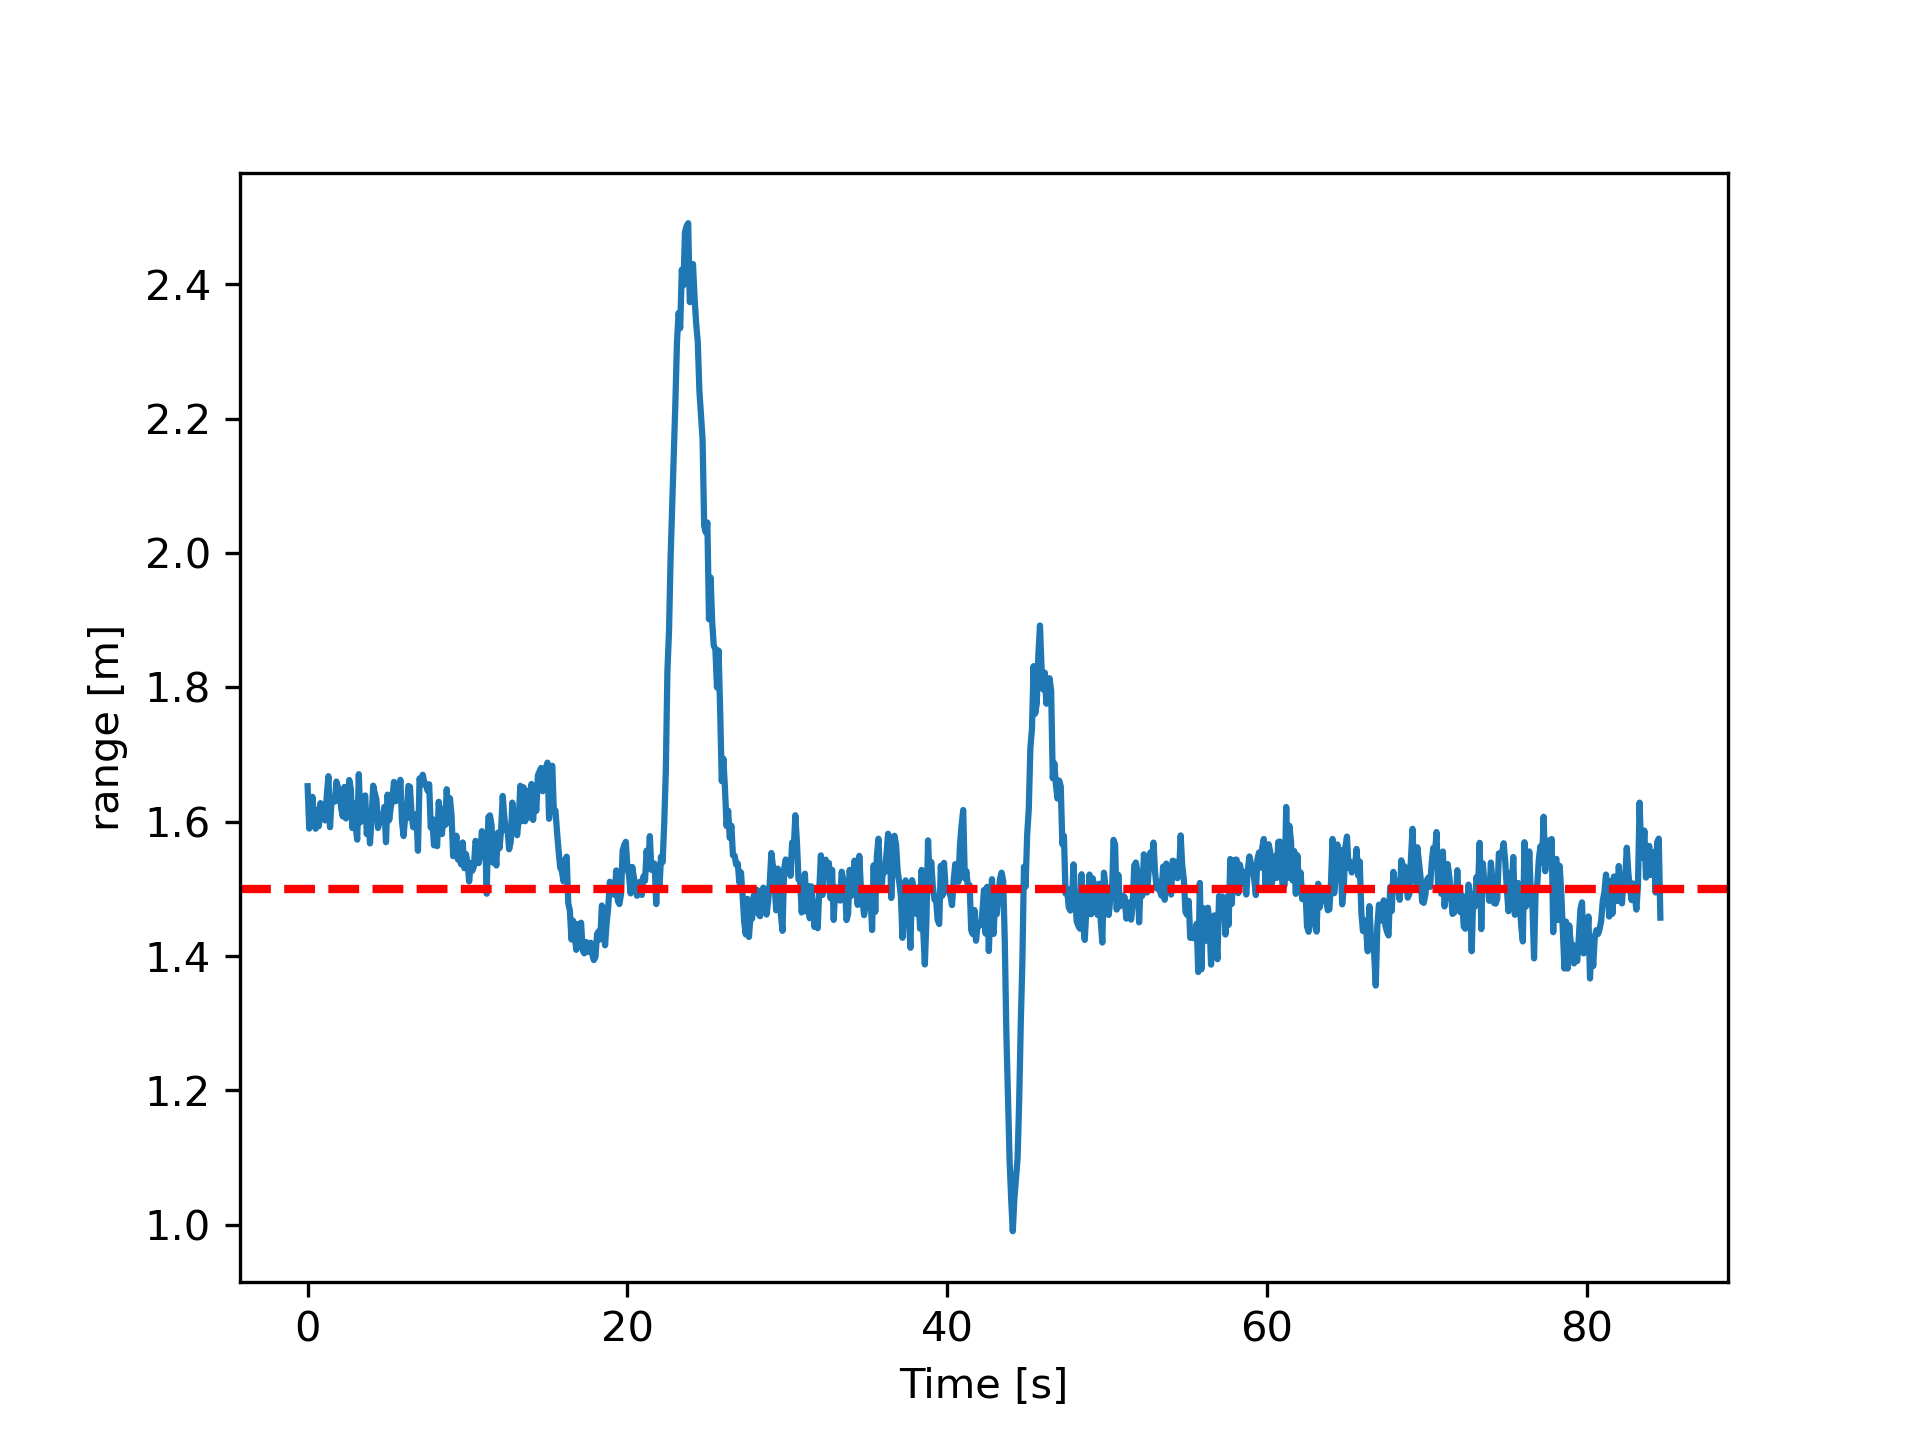
\includegraphics[width=0.48\textwidth]{images/Simulation/Range measures.png}
    \caption{Measured range in simulation. The red dotted line, indicates the wanted range from the following policy.}
    \label{SIM:range in time}
\end{figure}

\begin{figure}
    \centering
    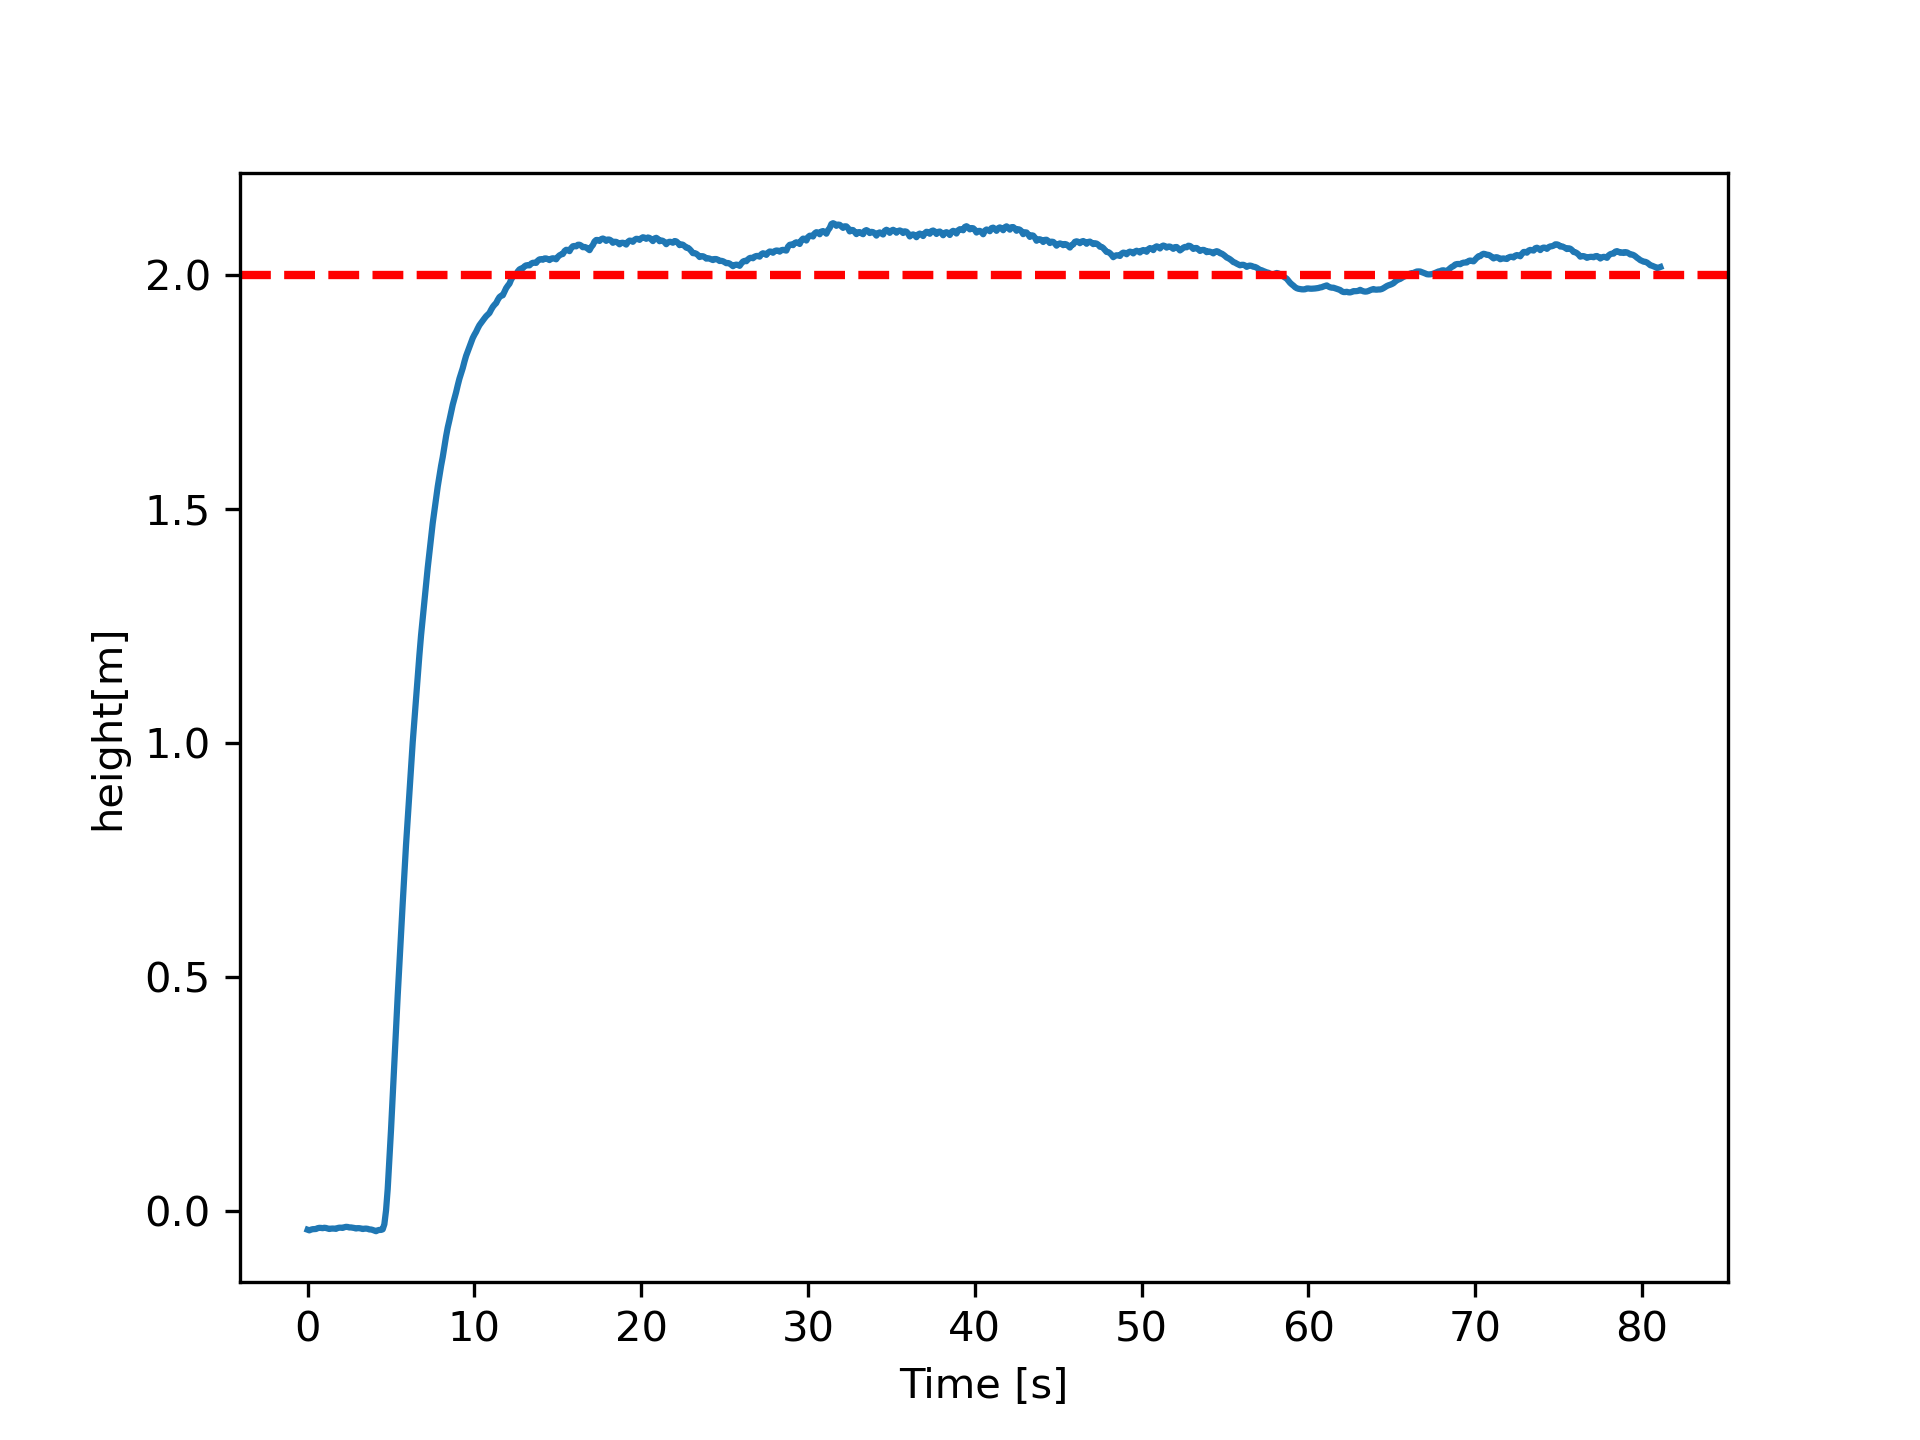
\includegraphics[width=0.48\textwidth]{images/Simulation/height_from_px4.png}
    \caption{Measured flight height in simulation. The red dotted line, indicates the wanted height from the following policy.}
    \label{SIM:height in time}
\end{figure}

The AoA sensed by the sensor during the motion is visible in \autoref{SIM:aoa in time}. After the first phase of takeoff and stabilization behind the target, it is possible to see that the measured angle is almost always inside a interval of $\pm 15$ degrees, except in the case of the sharp change of direction made when the curved motion starts. During the curves the quadcopter is not able to obtain a sensed angle of $0$, however the angle achieved is sufficiently low. A precisation that has to be done is that at the points after $50$ seconds where seems that a sudden change happens, it is due to the use of the function atan2 in calculations. Those are the points where the target y position changes sign, but the angle during the curves is stabilized around $10$ degrees, actually. \\

\begin{figure}
    \centering
    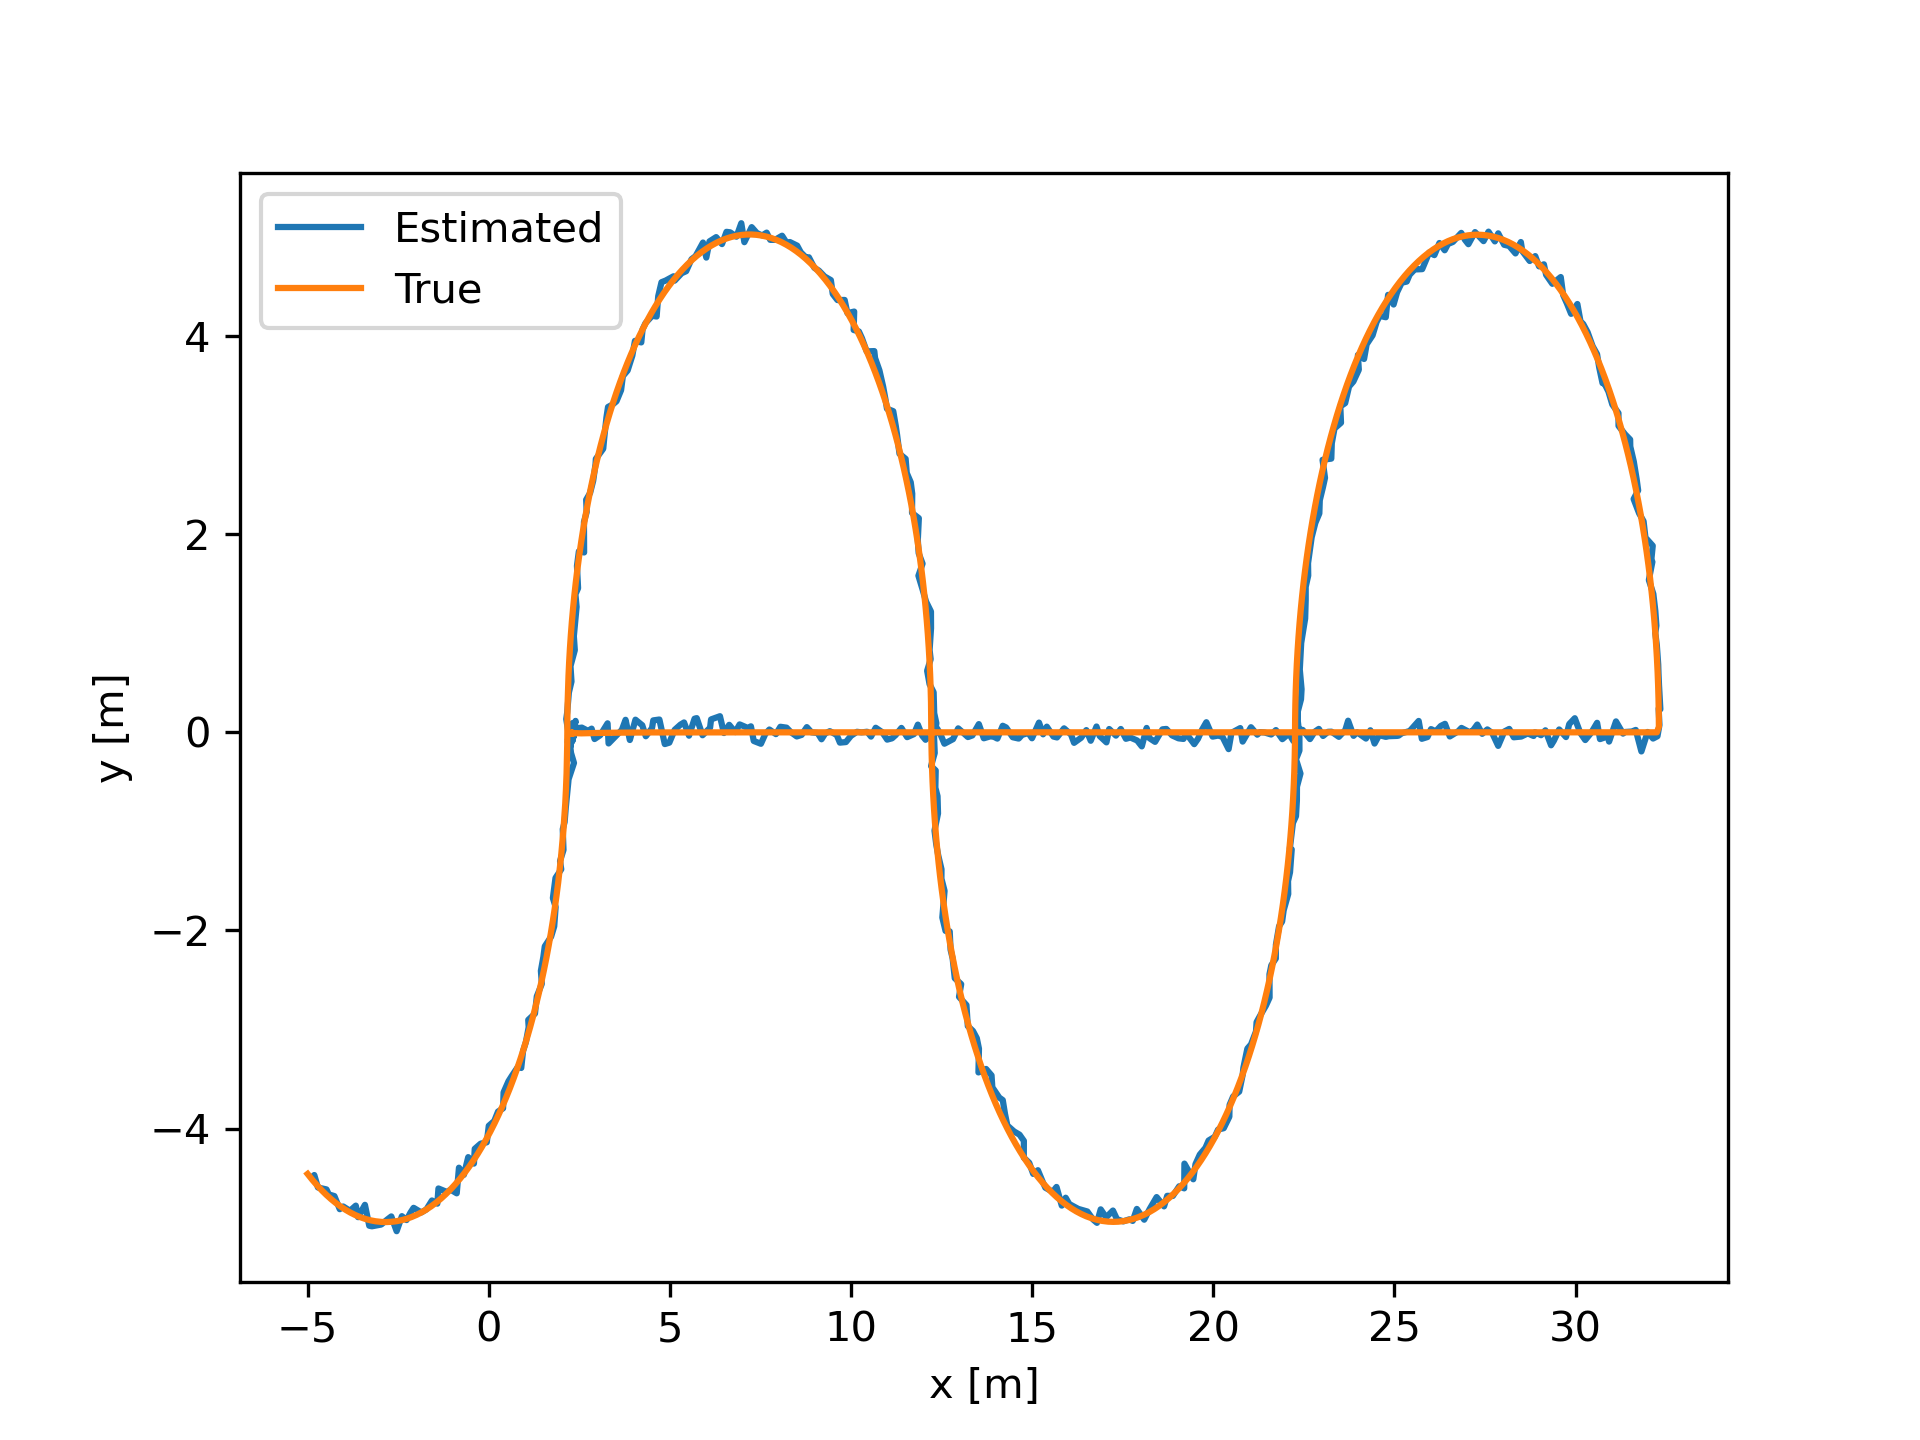
\includegraphics[width=0.48\textwidth]{images/Simulation/tag_estimation_vs_real.png}
    \caption{True and estimated pose of the target.}
    \label{SIM:target estimation}
\end{figure}

\begin{figure}
     \centering     
     \subfigure[]{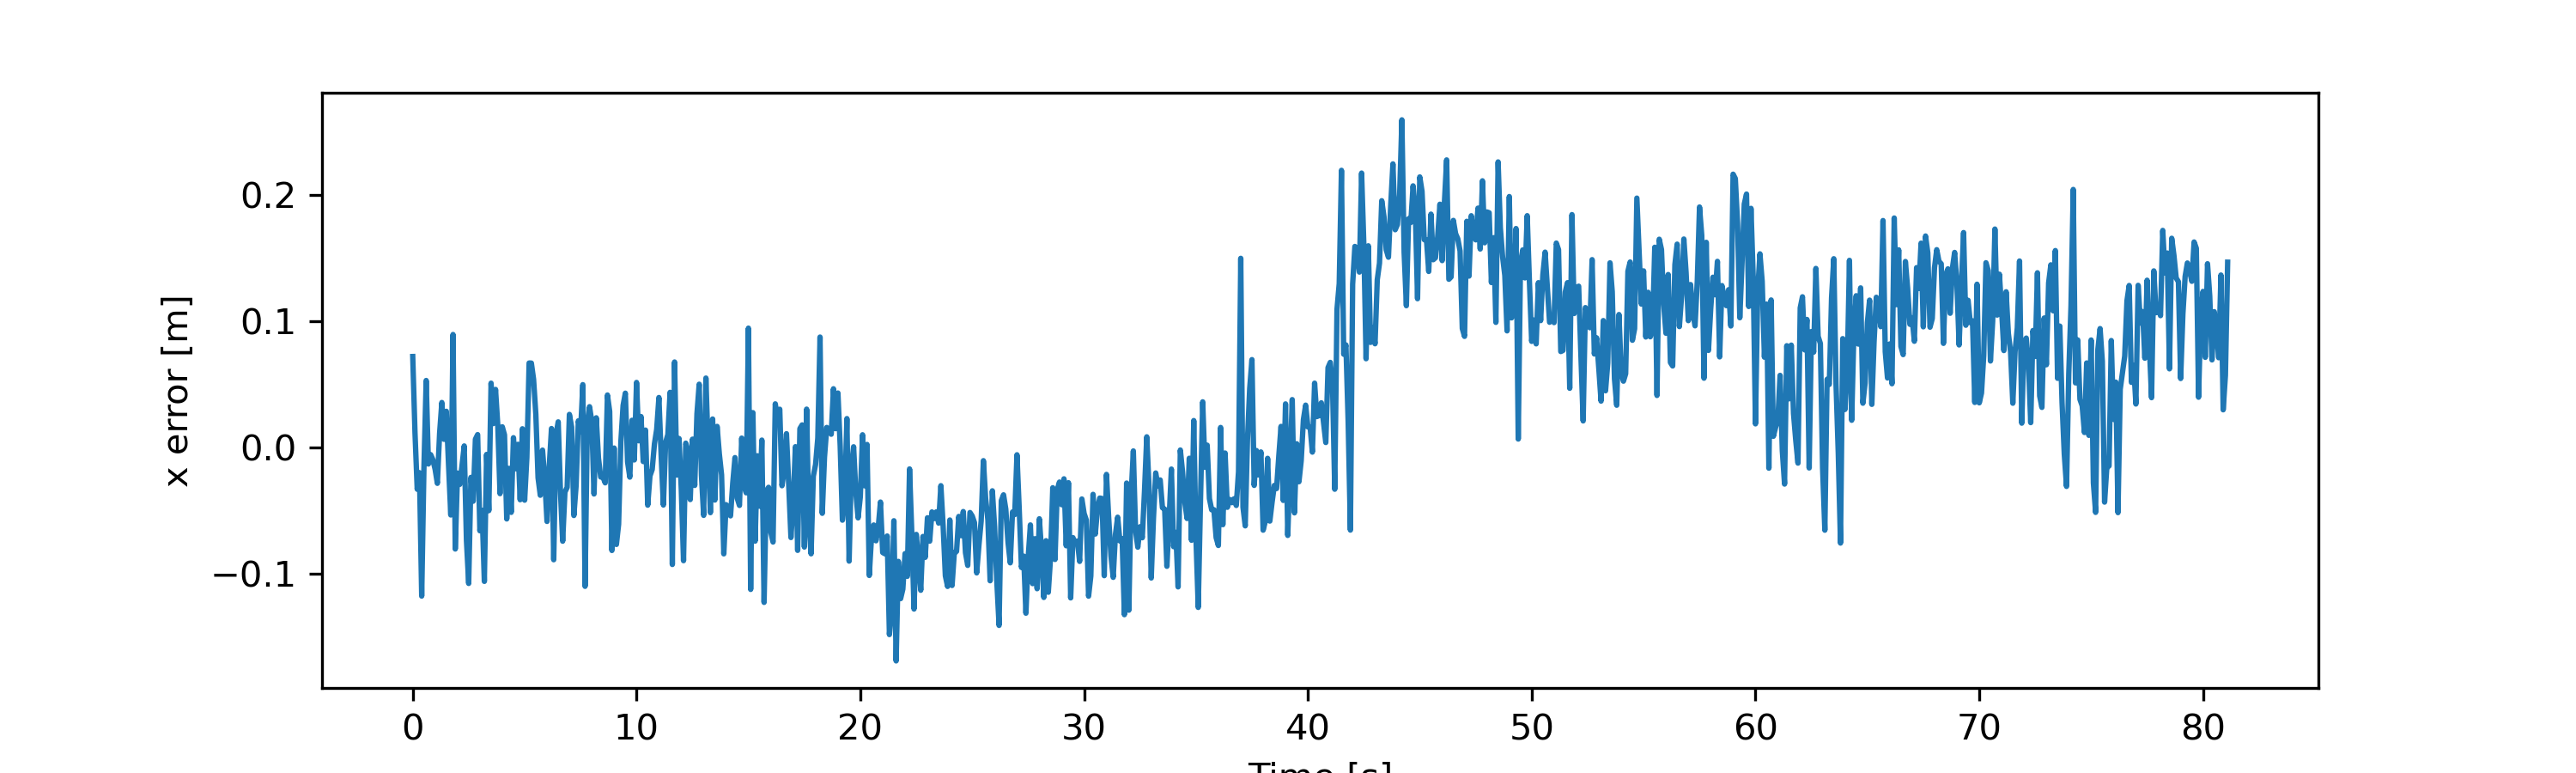
\includegraphics[width=0.48\textwidth]{images/Simulation/tag_estimation_errx.png}}\\
     \subfigure[]{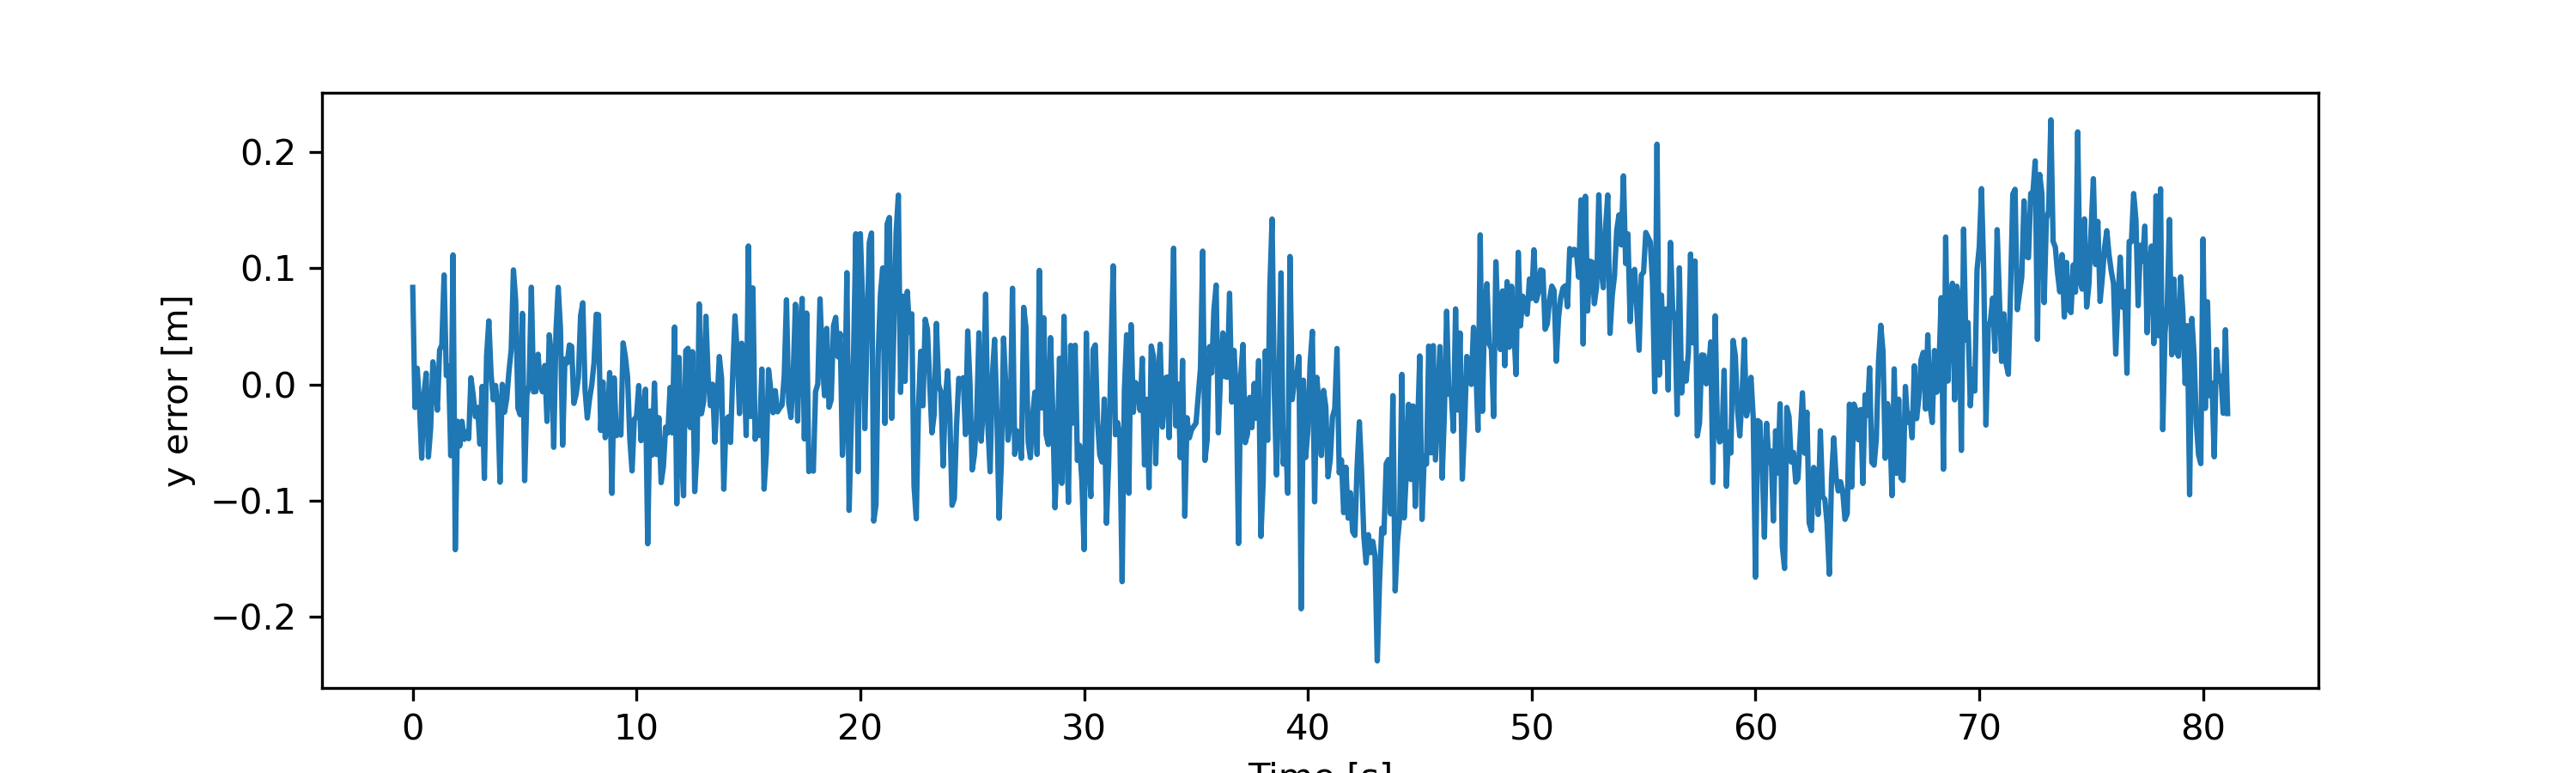
\includegraphics[width=0.48\textwidth]{images/Simulation/tag_estimation_erry.png}}
     \caption{(a) target localization x error [m]. (b) target localization y error [m].}
     \label{SIM:loc err}
\end{figure}

To evaluate the performance for what concerns the following distance, \autoref{SIM:range in time} can be considered. It can be seen that on average the demanded following distance is achieved. The peak around $20$ seconds is due to the target acceleration, that instantaneously pass from a static state, to move at the set velocity. Of course the designed PID controller do not stabilize at the same rate, so the peak is created. Instead the negative-positive peak pair around $40$ seconds is caused by the target's change of direction. In that moment the quadcopter stops and waits due to the presence of the integral control effect on the velocity setpoint generation, necessary to have a following distance without bias, counteracting the proportional control behaviour. Without the integral control, the proportional would cause the quadcopter to move backwards at that moment, mitigating that peak pair. However, exception made for this extreme case, our strategy seems to be appropriate so we decided to use the integral, although in some cases it may imply lowerings of the following distance. For safety purposes, in order to mitigate this effect while keeping the integral effect, some other strategies should be investigated.\\

\begin{figure}
    \centering
    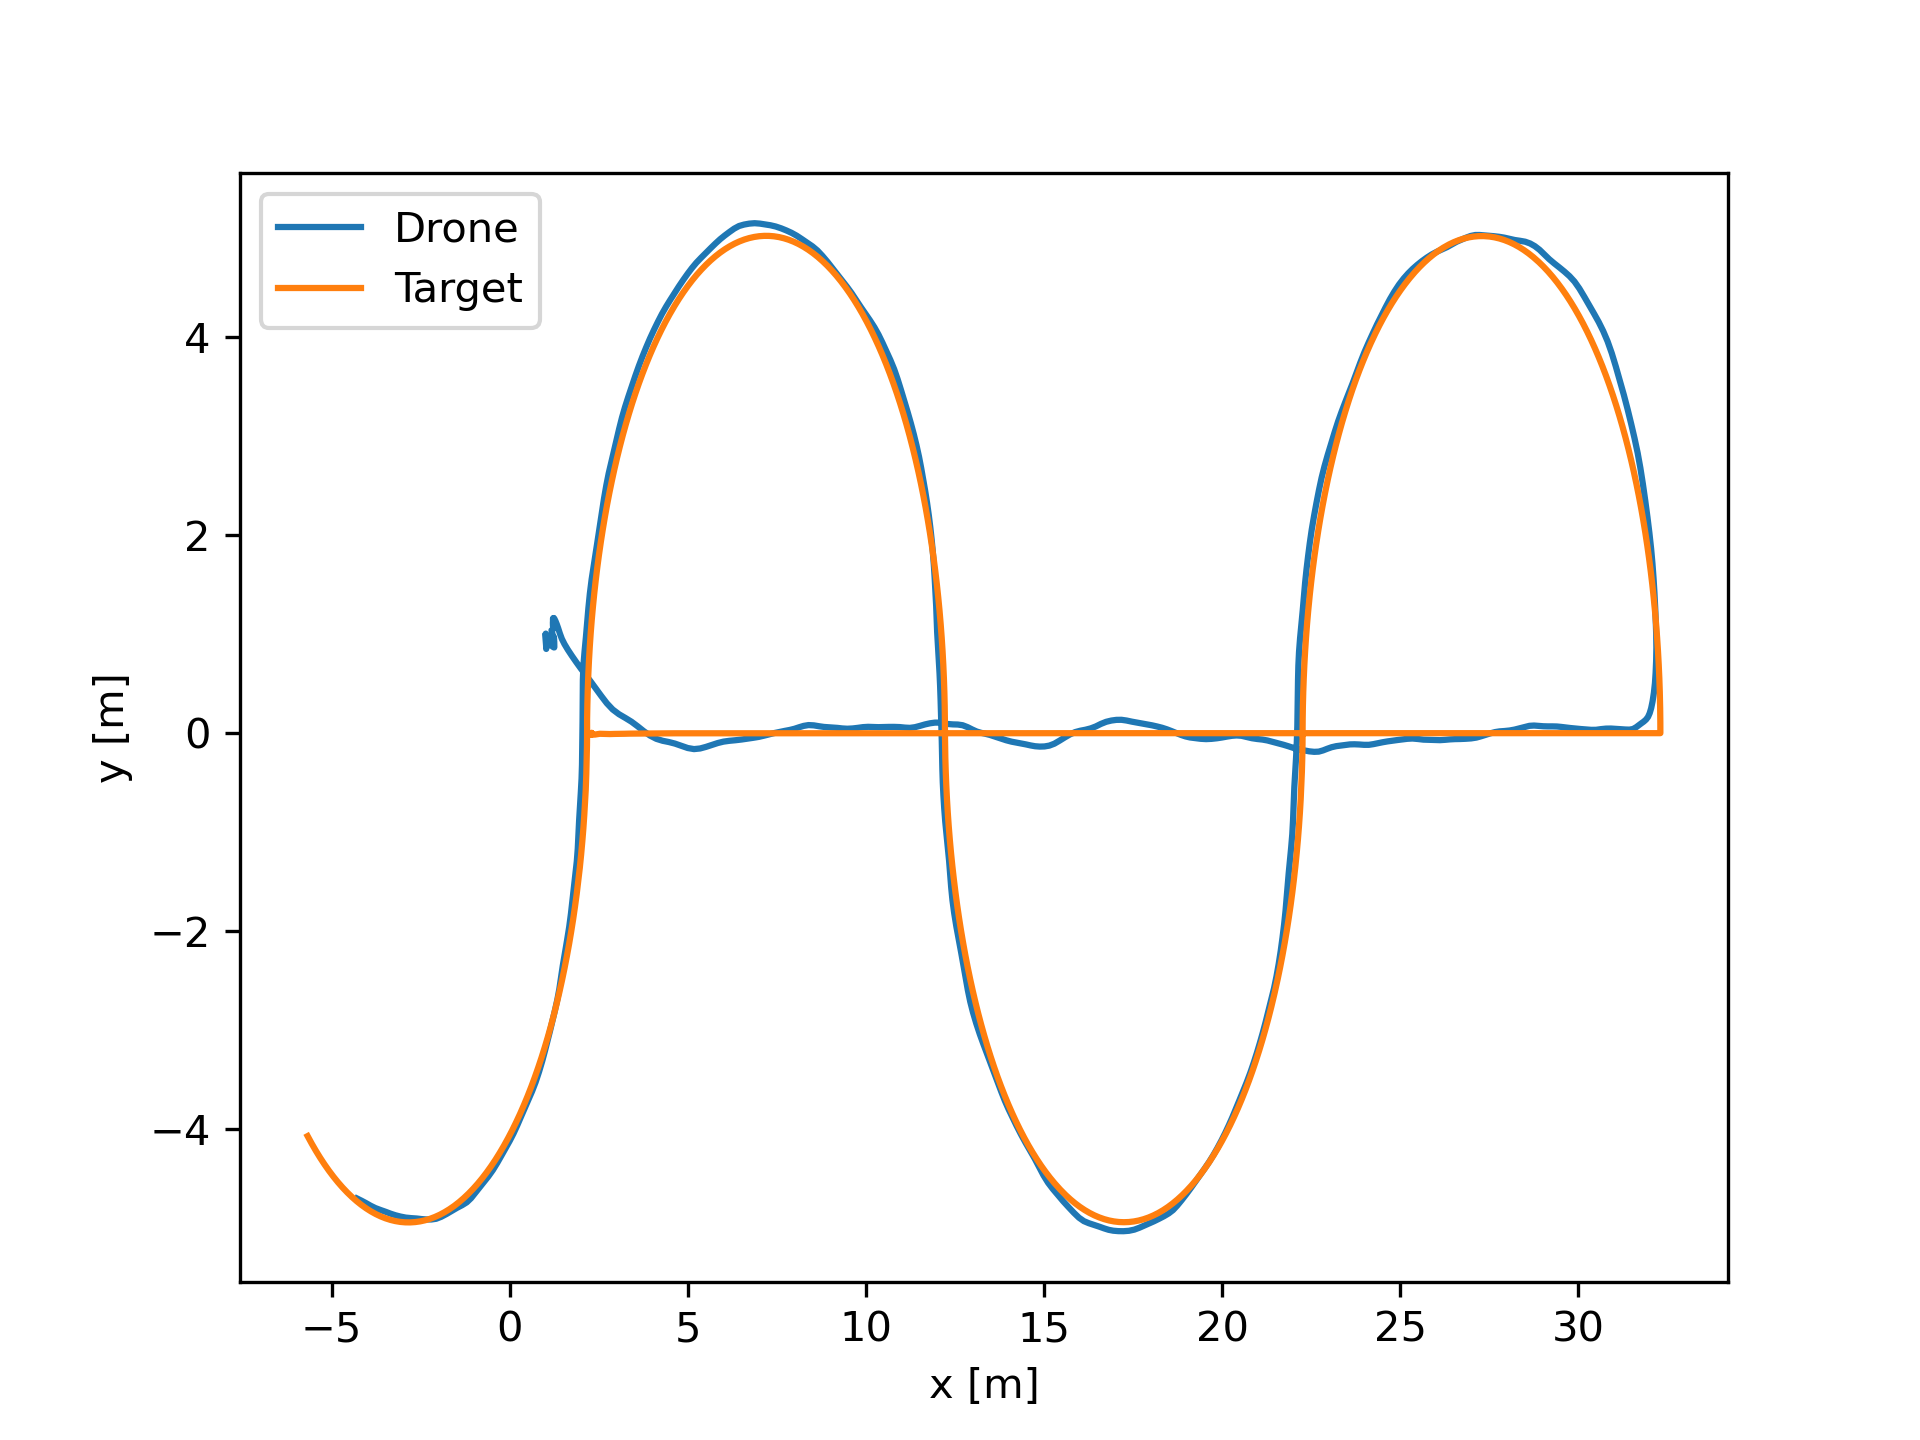
\includegraphics[width=0.48\textwidth]{images/Simulation/Drone_Target x-y Position_noisy.png}
    \caption{Target and drone trajectory in simulation with high noise.}
    \label{SIM:traj_noisy}
\end{figure}

\begin{figure}
    \centering
    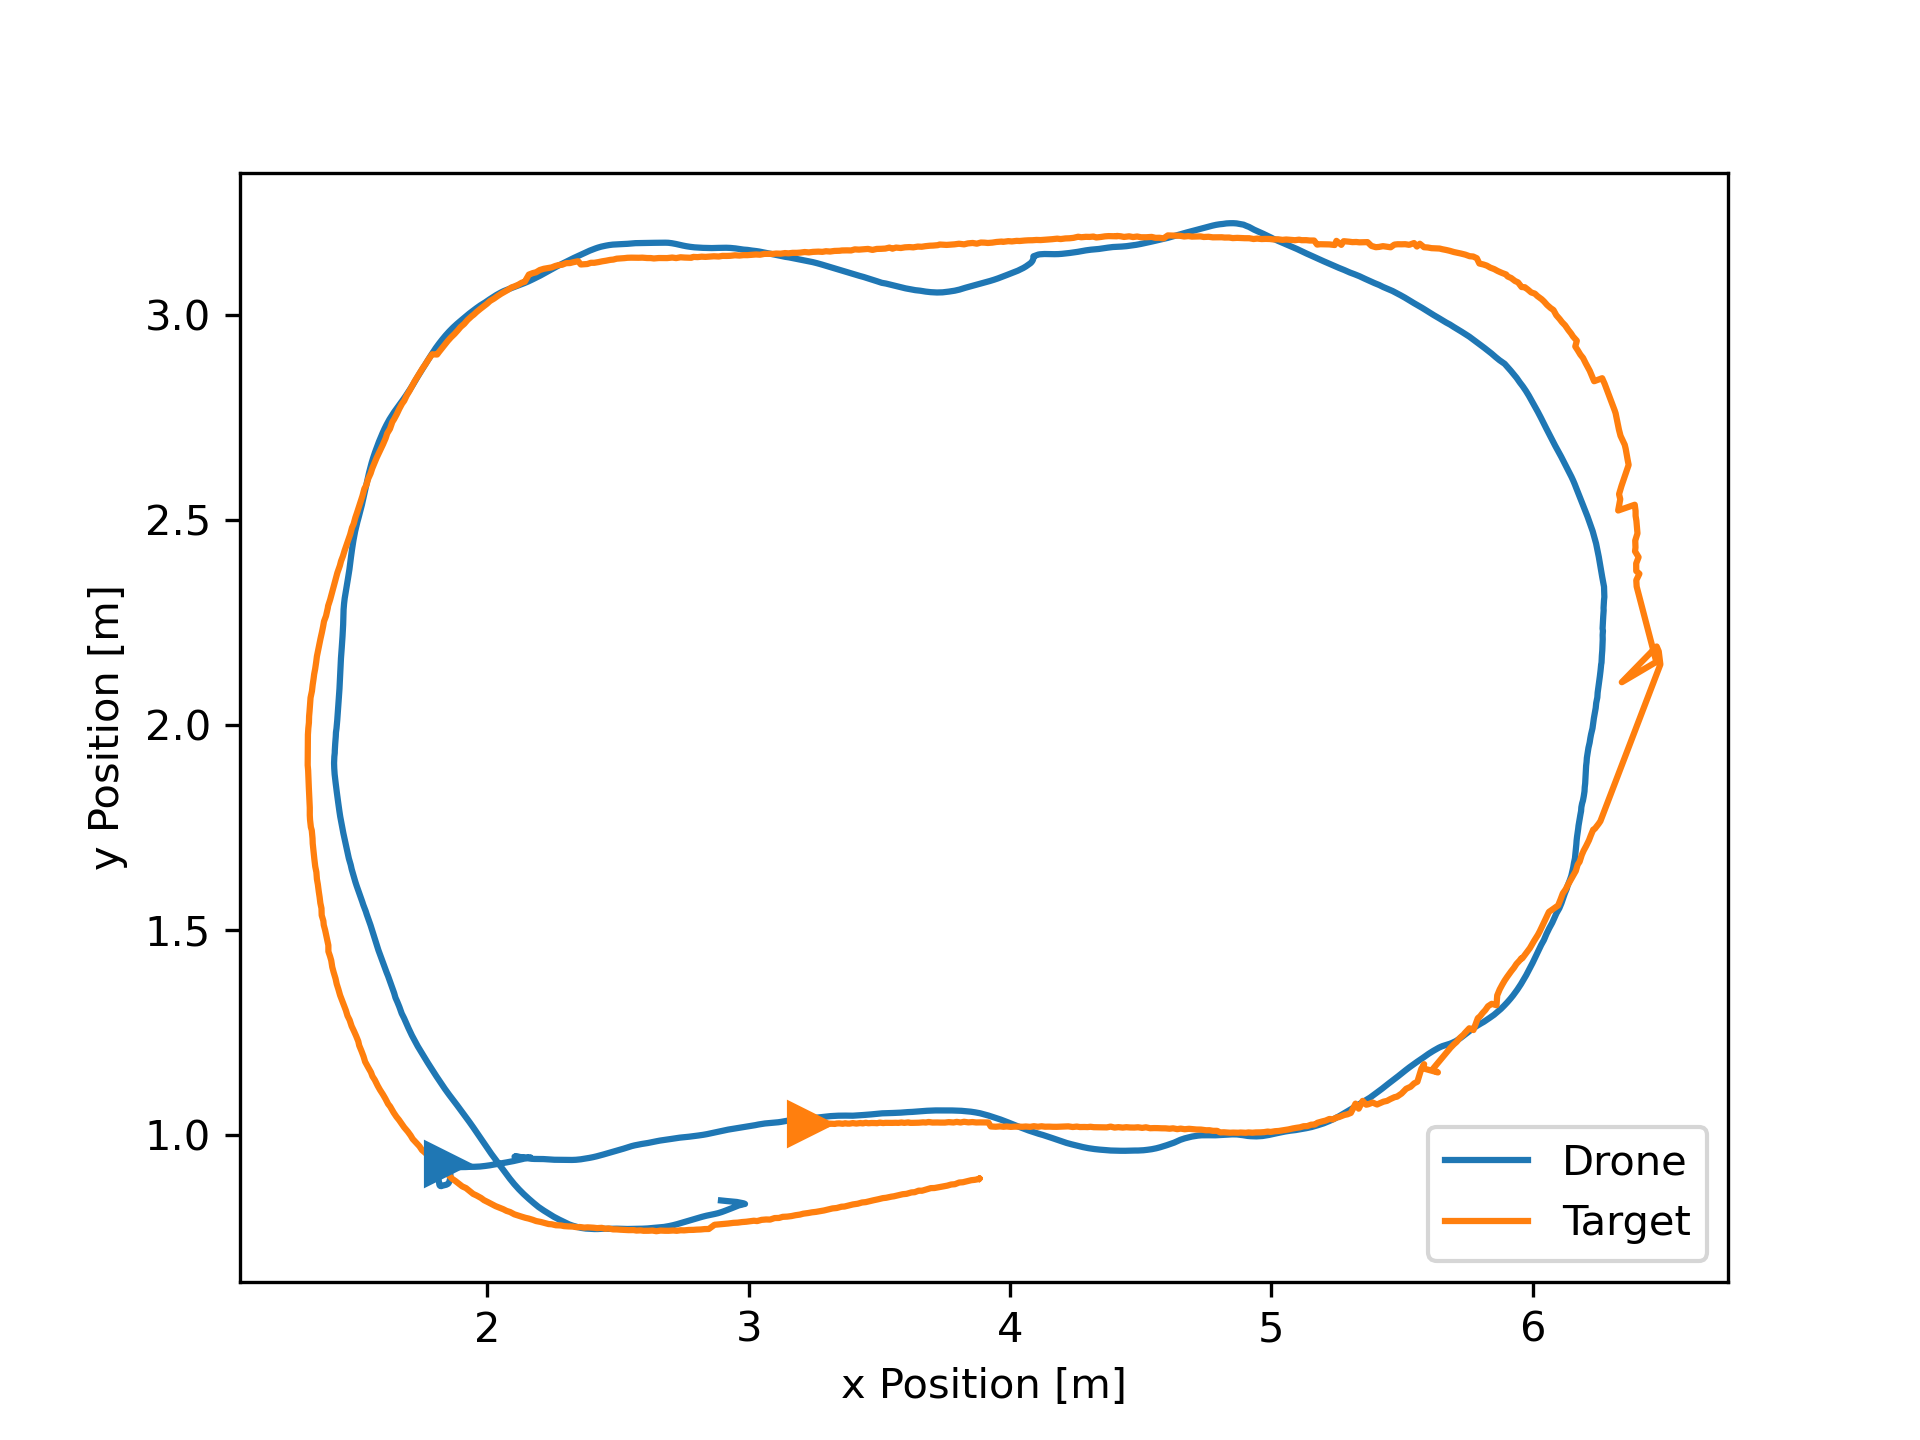
\includegraphics[width=0.48\textwidth]{images/real_test/drone_target_xy_pos.png}
    \caption{Target and drone trajectory in real test.}
    \label{REAL:fig:traj}
\end{figure}

Even the flight height is well respected, as can be seen in \autoref{SIM:height in time} and it seems to be independent w.r.t. events such as motion type changes. 
The accuracy of the estimation of the target position in the global frame done by the quadcopter using the UWB sensor is shown in \autoref{SIM:target estimation}, and it can be noted that is always reliable. More in detail, this can be seen in particular in \autoref{SIM:loc err}. The error is never greater than $0.3$ meters for both the axis. It can also be seen that is dependent on the type of motion: in the first phase, where there is only straight motion the error is low and approximately null on average. At the moment of the change of direction, it expands, for both the axis and the mean done on a window relative to that moment is not null. However, the fact that the error is never too large guarantees acceptable following performance if the control strategy is appropriate. \\
To test the robustness of the following system, a simulation with noises affected by larger standard deviations, $10$ centimeters for the range and $10$ degrees for the AoA was performed. From \autoref{SIM:traj_noisy}, it can be seen that the quadcopter is still able to execute its task, albeit roughly. \\
Overall these results suggests that our strategy works, at least in the simulated conditions: some effects indeed are neglected, as the fact that the real quadcopter available to us is smaller and different to the simulated Iris drone as well as the inertial modifications due to the mounted UWB sensor, that are not considered. 

\begin{figure}
    \centering
    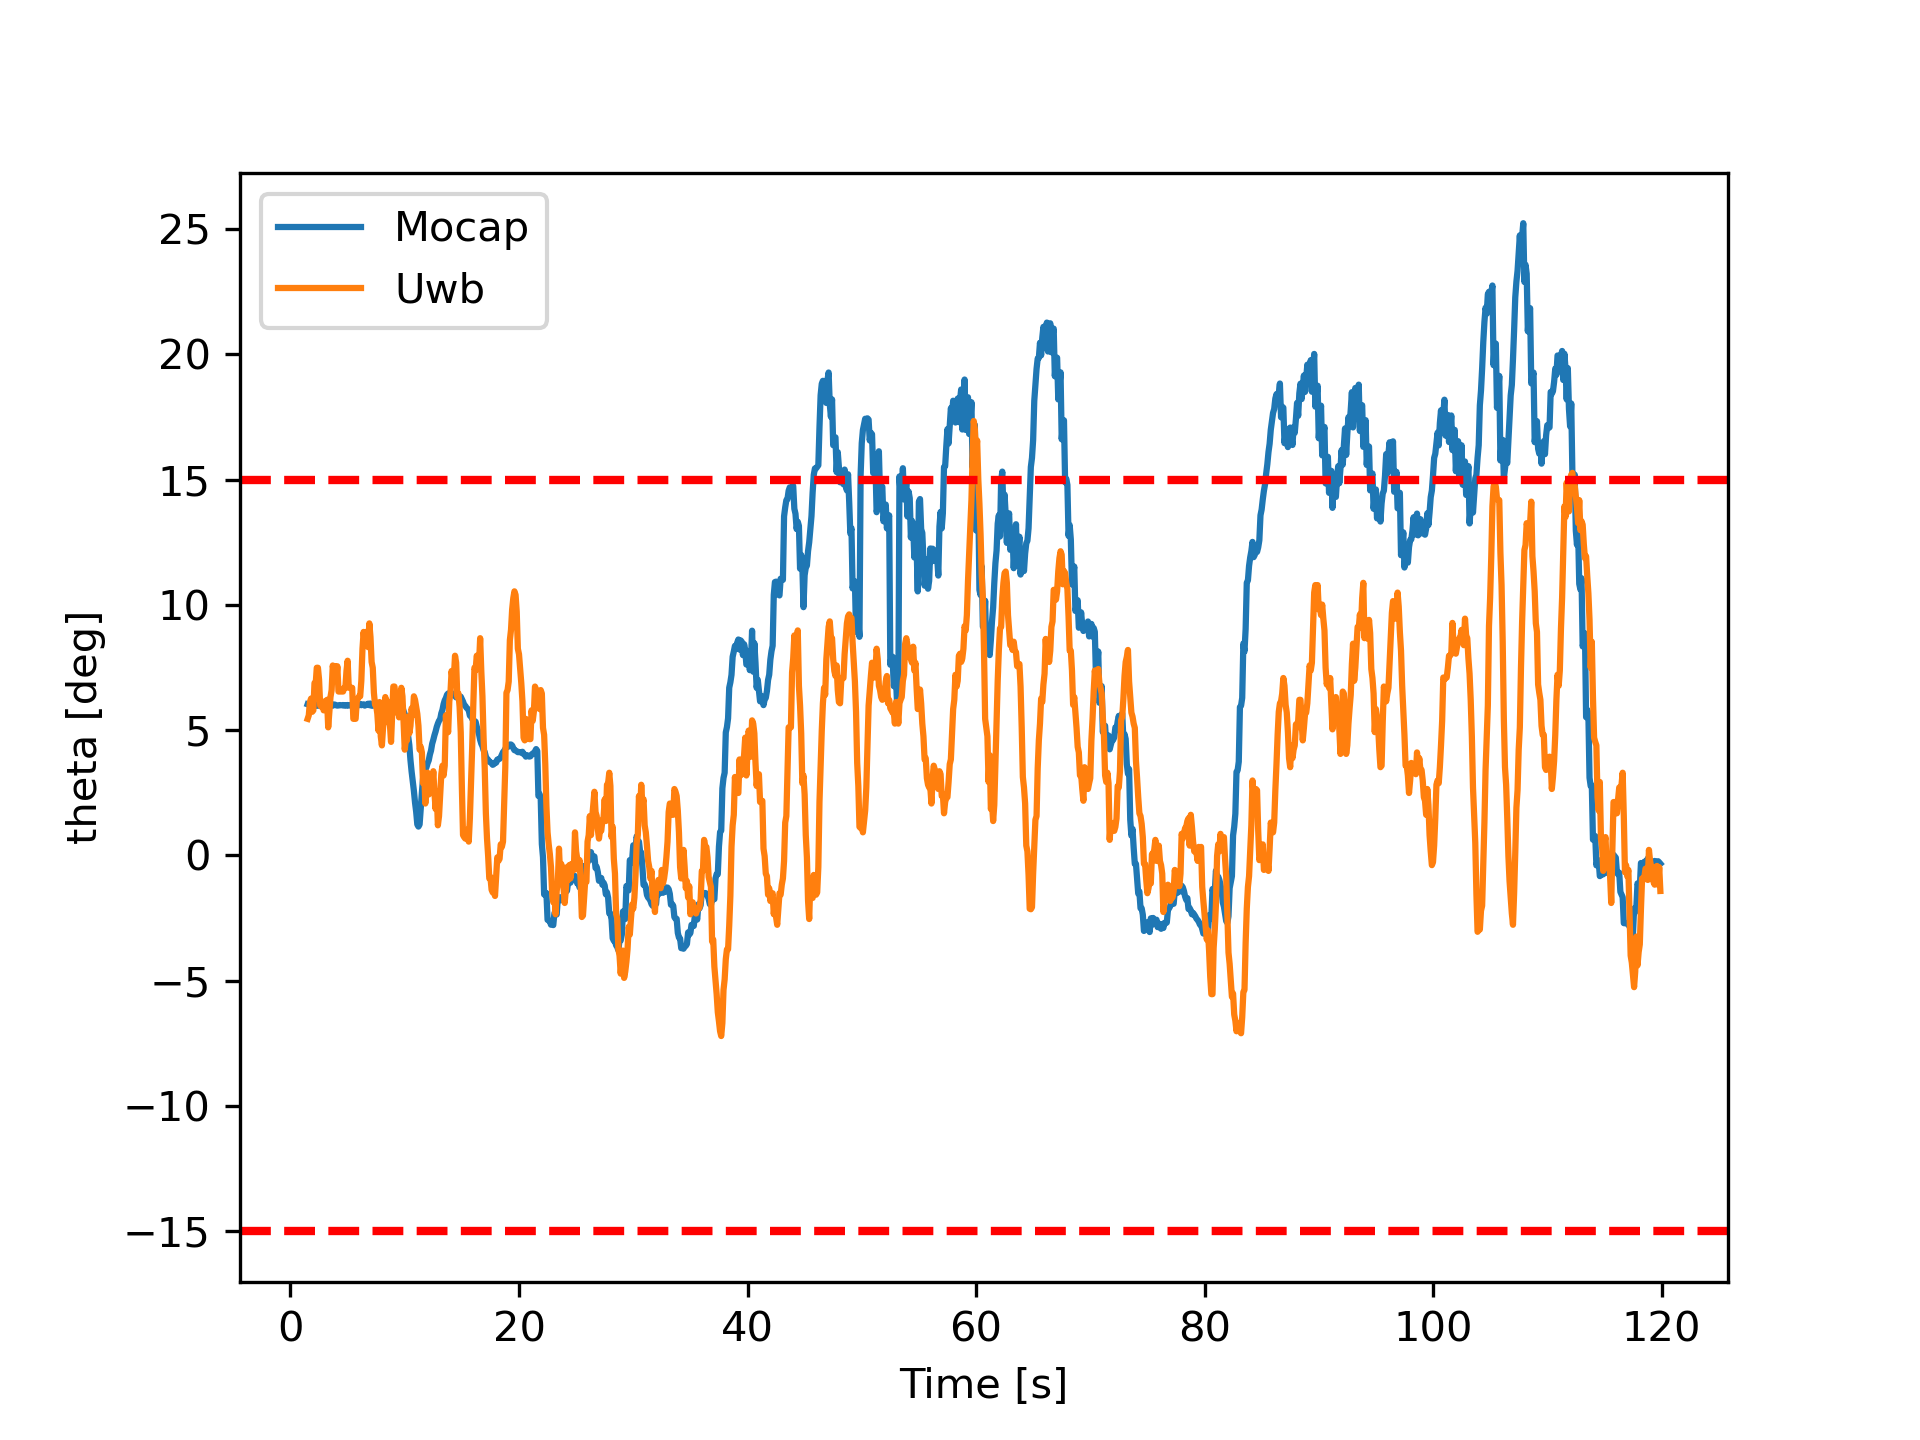
\includegraphics[width=0.48\textwidth]{images/real_test/aoa_Uwb_Mocap.png}
    \caption{angle of arrival between drone and target. The sensor measure, is compered with the one obtained with MoCap. The red dotted line, indicates the wanted range from the following policy}
    \label{REAL:fig:aoa}
\end{figure}

\begin{figure}
    \centering
    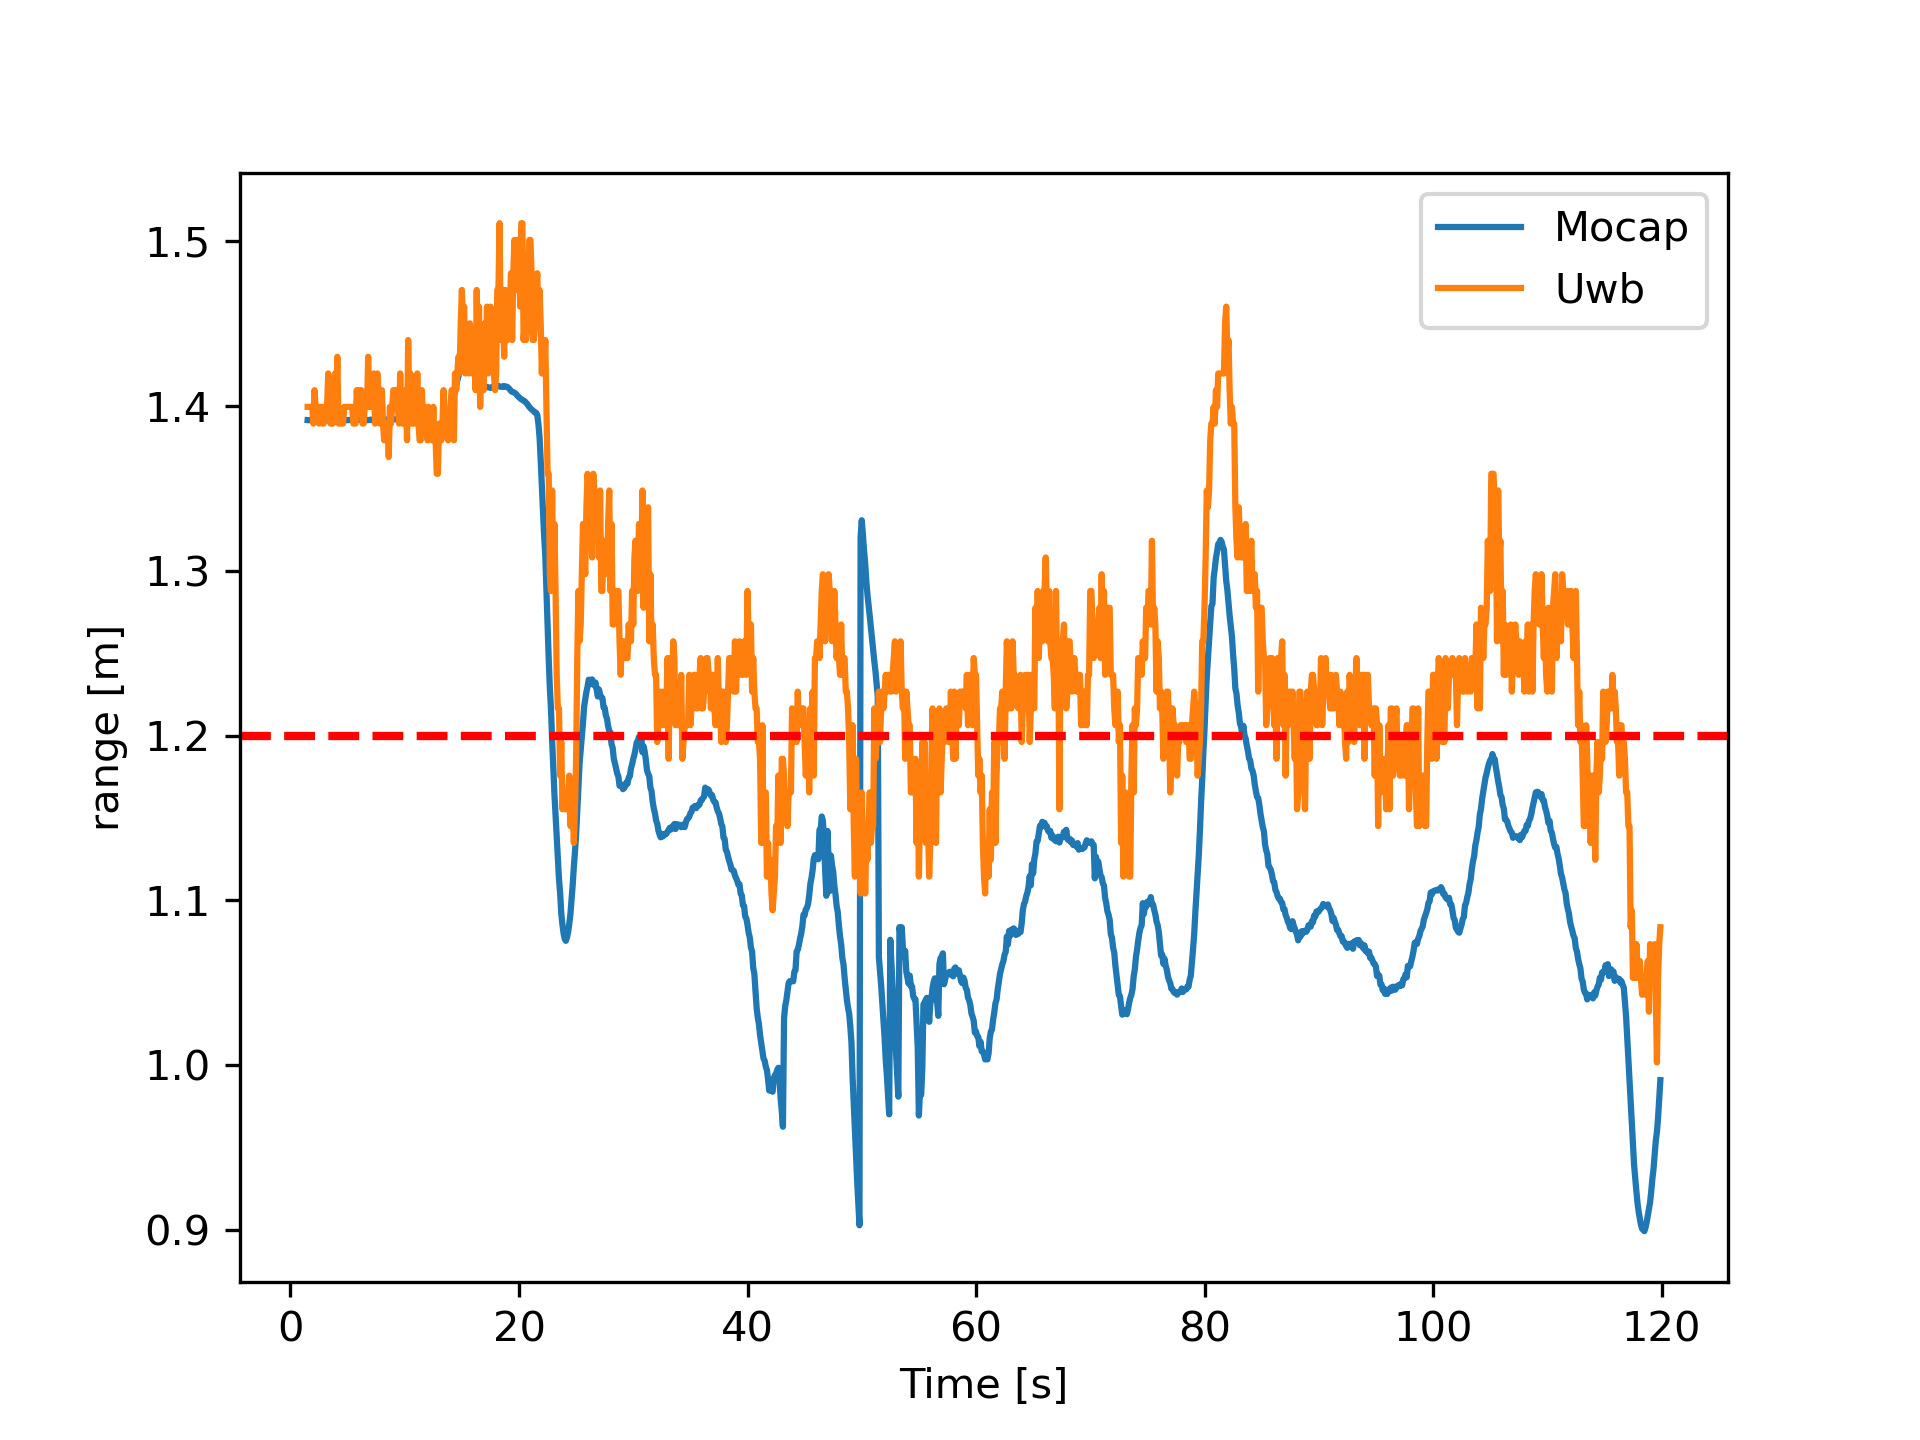
\includegraphics[width=0.48\textwidth]{images/real_test/range_Uwb_Mocap.png}
    \caption{Range between drone and target. The sensor measure, is compered with the one obtained with MoCap.}
    \label{REAL:fig:range}
\end{figure}

\subsection{Real test}
To test the validity of the UWB kit in a real application, and to further prove the effectiveness of the following algorithm, as previously explained, some real tests where performed. All the presented results are paired with the relative MoCap ground truth for comparison. The presented results are the best of the conducted tests. In order to obtain a decent motion inside the restricted Mocap laboratory environment, the test is conducted choosing a drone flight height of $0.4$ meters (to ensure marker visibility) and a following distance of $1.2$ meters. This choice is for sure restricting the UWB kit performance, since better results are obtained at larger distances (as suggested by the manufacturer), but this choice is restricted by the lab dimensions that do not allow to perform good trajectories with higher distances. In \autoref{REAL:fig:traj} the trajectory of both drone and target, given by MoCap, are presented. It is clear that the drone almost follow the square-like trajectory of the target, suggesting the effectiveness of the following strategy. For what concerns the policy compliance, in \autoref{REAL:fig:aoa}, \ref{REAL:fig:range} AoA and range obtained by the sensor with the relative MoCap ground truth, are depicted. From both can be highlighted the presence of a non-linear bias that majorly depends by the angle. This confirms the behaviour seen in the characterization, in which the angle bias is a function of the actual angle. Nonetheless, the error is maximum in the target turning phases, in which the DDR robot is turned with an almost sharped trajectory. This concertize the behavior mentioned in the characterization conclusions, for which the measure are worsen by a non radial facing of the tag w.r.t. the double UWB. All this effects sum up obtaining a non constant bias, especially for the AoA. Nevertheless, if we do not consider the biases, in general the policy is followed. Surely, an outdoor test performed in an open environment, with a more relaxed policy (i.e. a greater following distance), should achieve better results. For what concerns the height, as described, is controlled directly by sending constants z setpoints. The flight height followed by the quadcopter, is presented in \autoref{REAL:fig:height}. The height is maintained with an error similar to the one of the simulation.\\

\begin{figure}
    \centering
    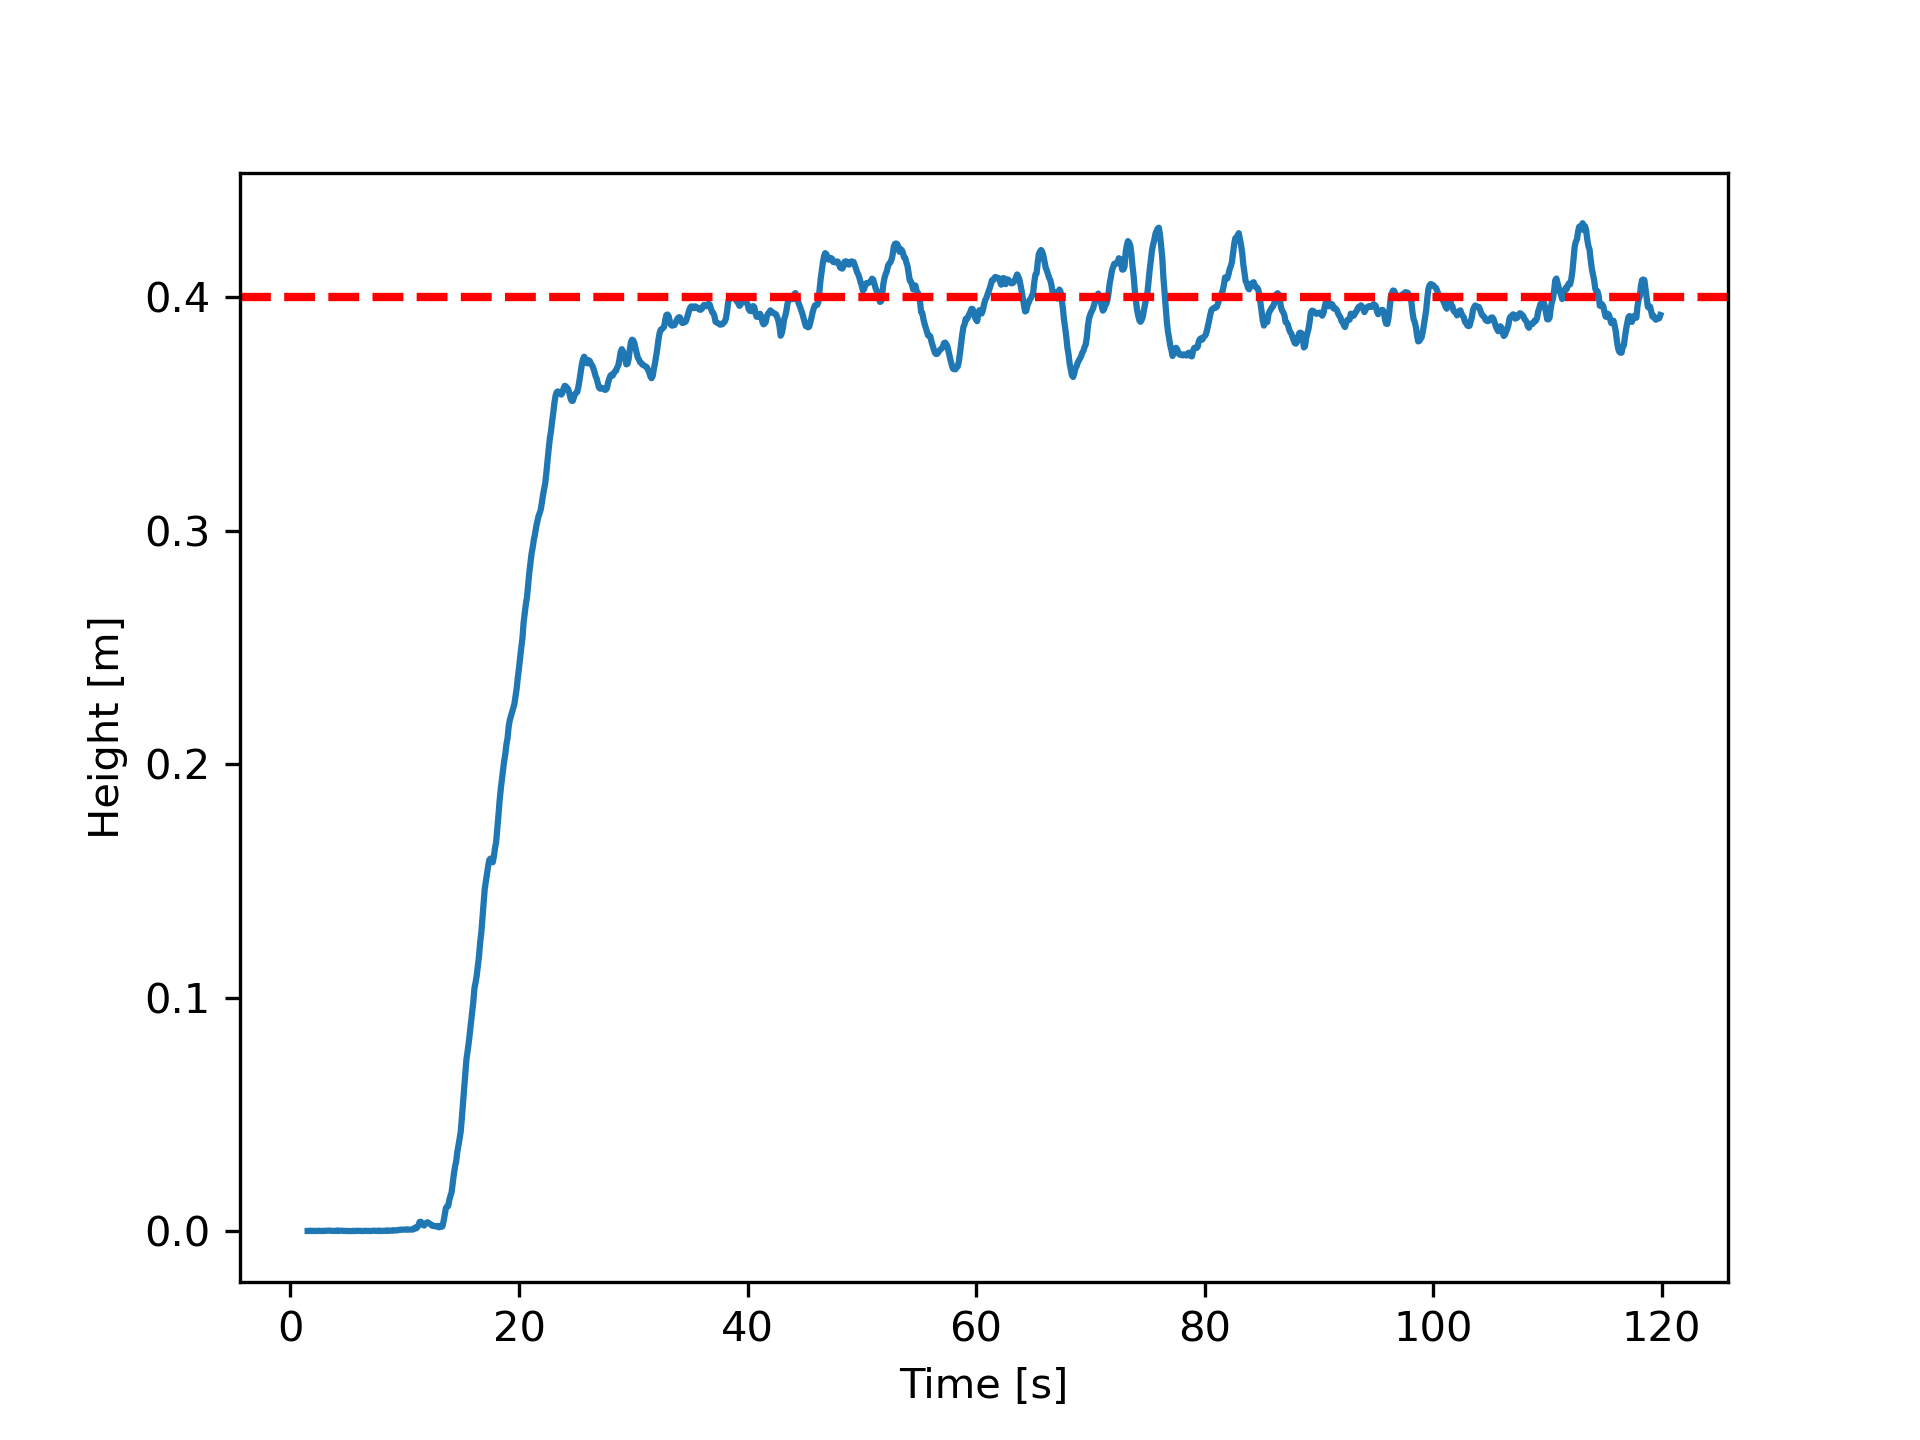
\includegraphics[width=0.48\textwidth]{images/real_test/drone_height.png}
    \caption{Measured flight height. The red dotted line, indicates the wanted height from the following policy.}
    \label{REAL:fig:height}
\end{figure}

\begin{figure}
    \centering
    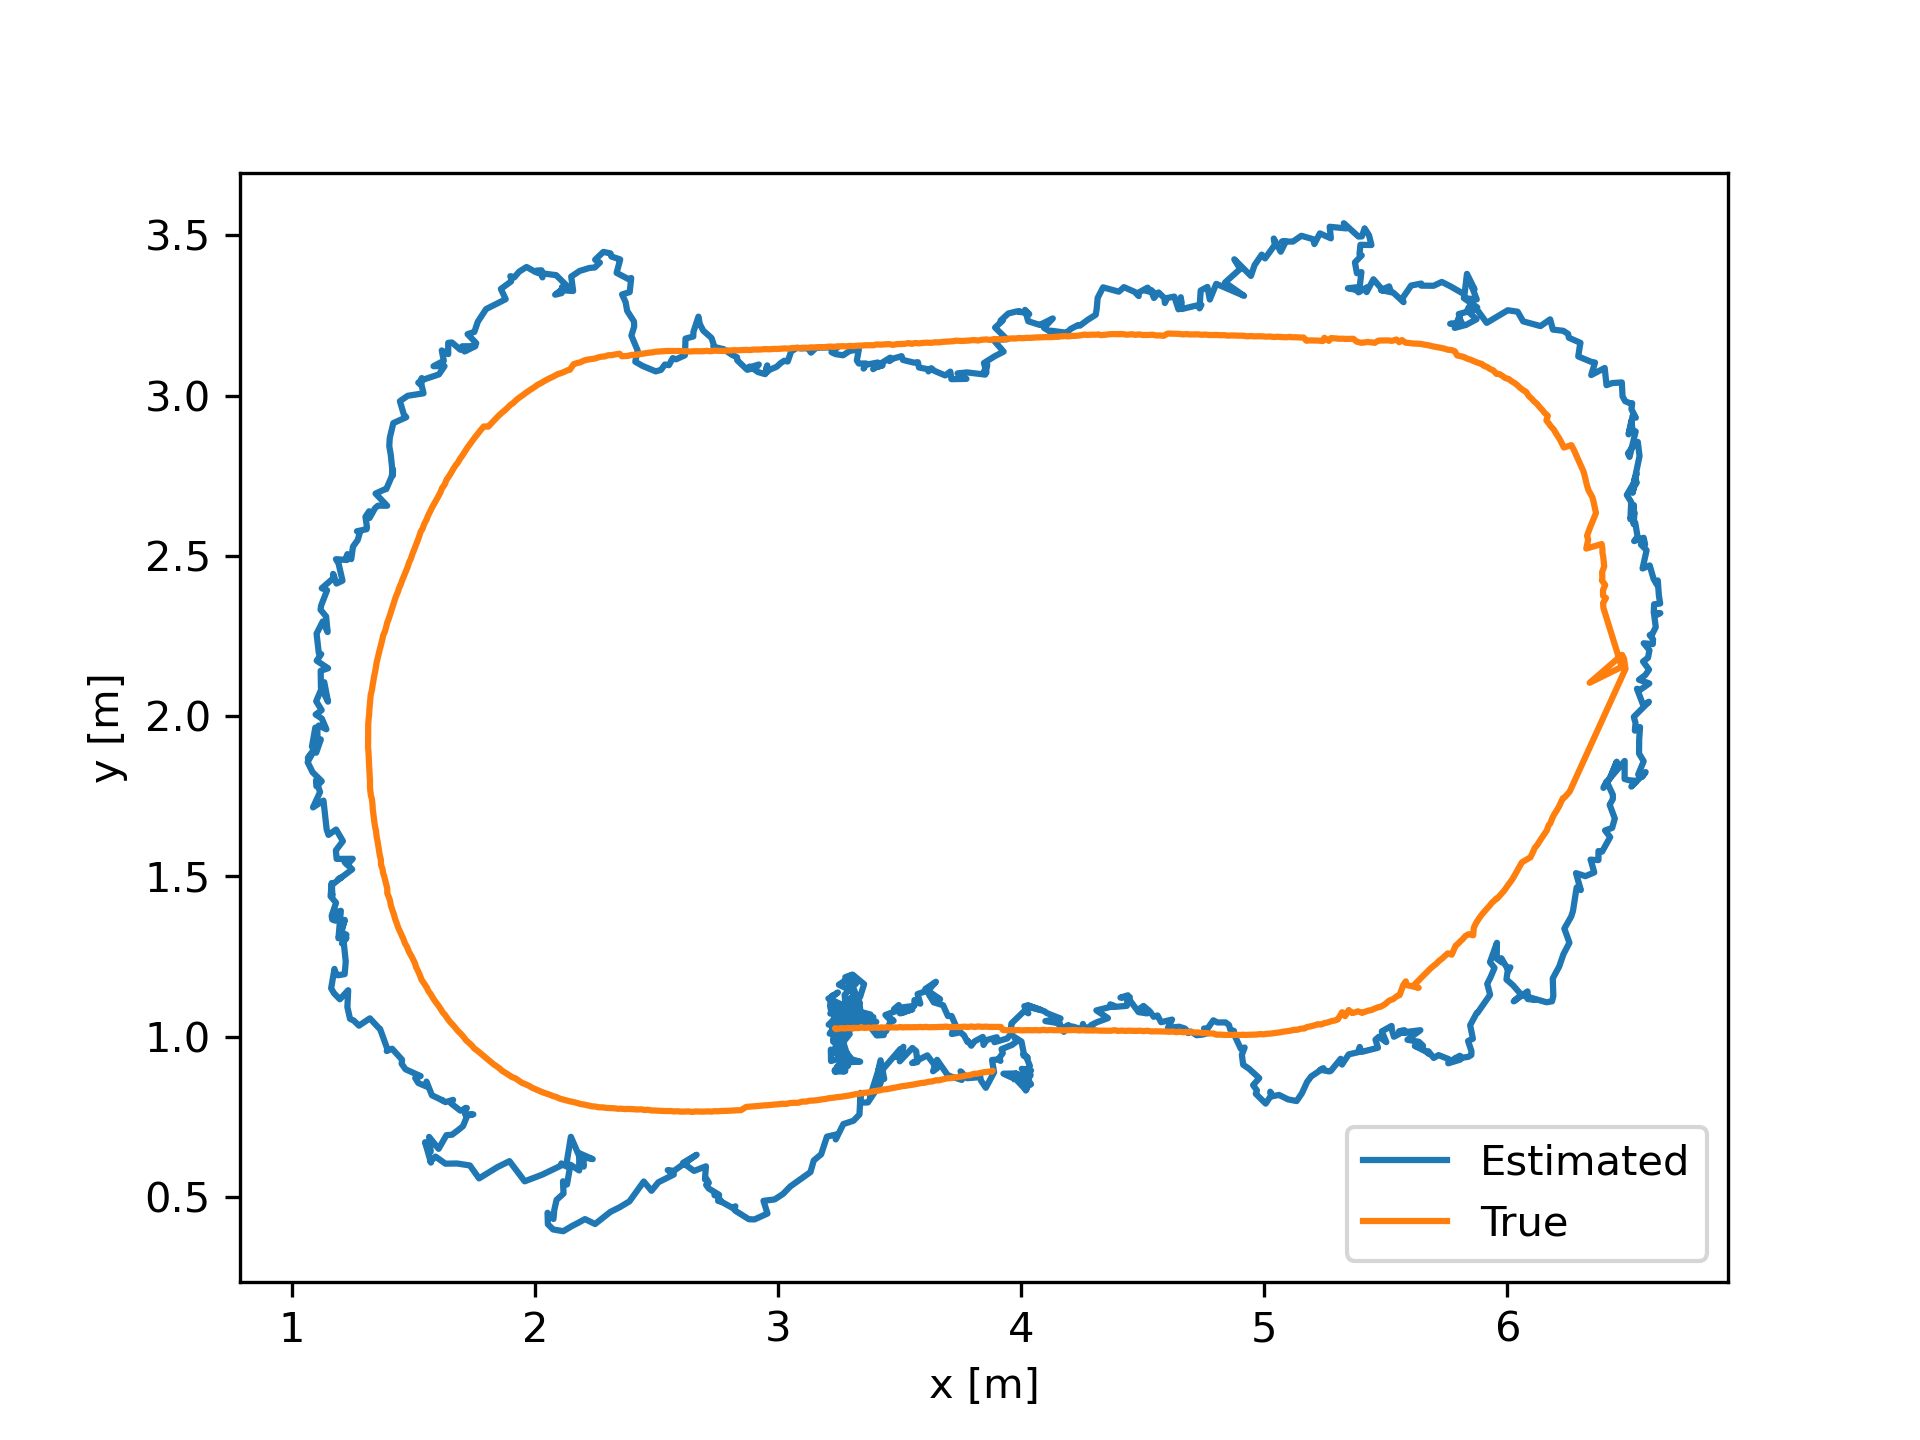
\includegraphics[width=0.48\textwidth]{images/real_test/tag_estim-real_pos.png}
    \caption{True and estimated pose of the target.}
    \label{REAL:fig:tag_estim}
\end{figure}

The accuracy of the target position drone's estimate, performed using the UWB sensor and its own position estimate, is shown in \autoref{REAL:fig:tag_estim}. As can be seen, the estimate follows in general the truth, but is clearly affected by the angle and range biases previously discussed. To better asses the localization performance, the x and y error in time are exposed in \autoref{REAL:fig:loc_err}. The error in both the axes, is bounded in $\pm 0.4$ meters, which is almost twice the one obtained in the simulation. This is clearly due to the described biases.\\

In conclusion this test brings up the UWB problems discussed in \autoref{UWB_CHAR}, affecting the final results. Overall the drone behaviour itself, is quite good, and the target localization remains bounded in an acceptable range. As stated, the performance could be better in larger environments with greater following distance. Further tests in this direction, are advised as future work.

\begin{figure}
     \centering     
     \subfigure[]{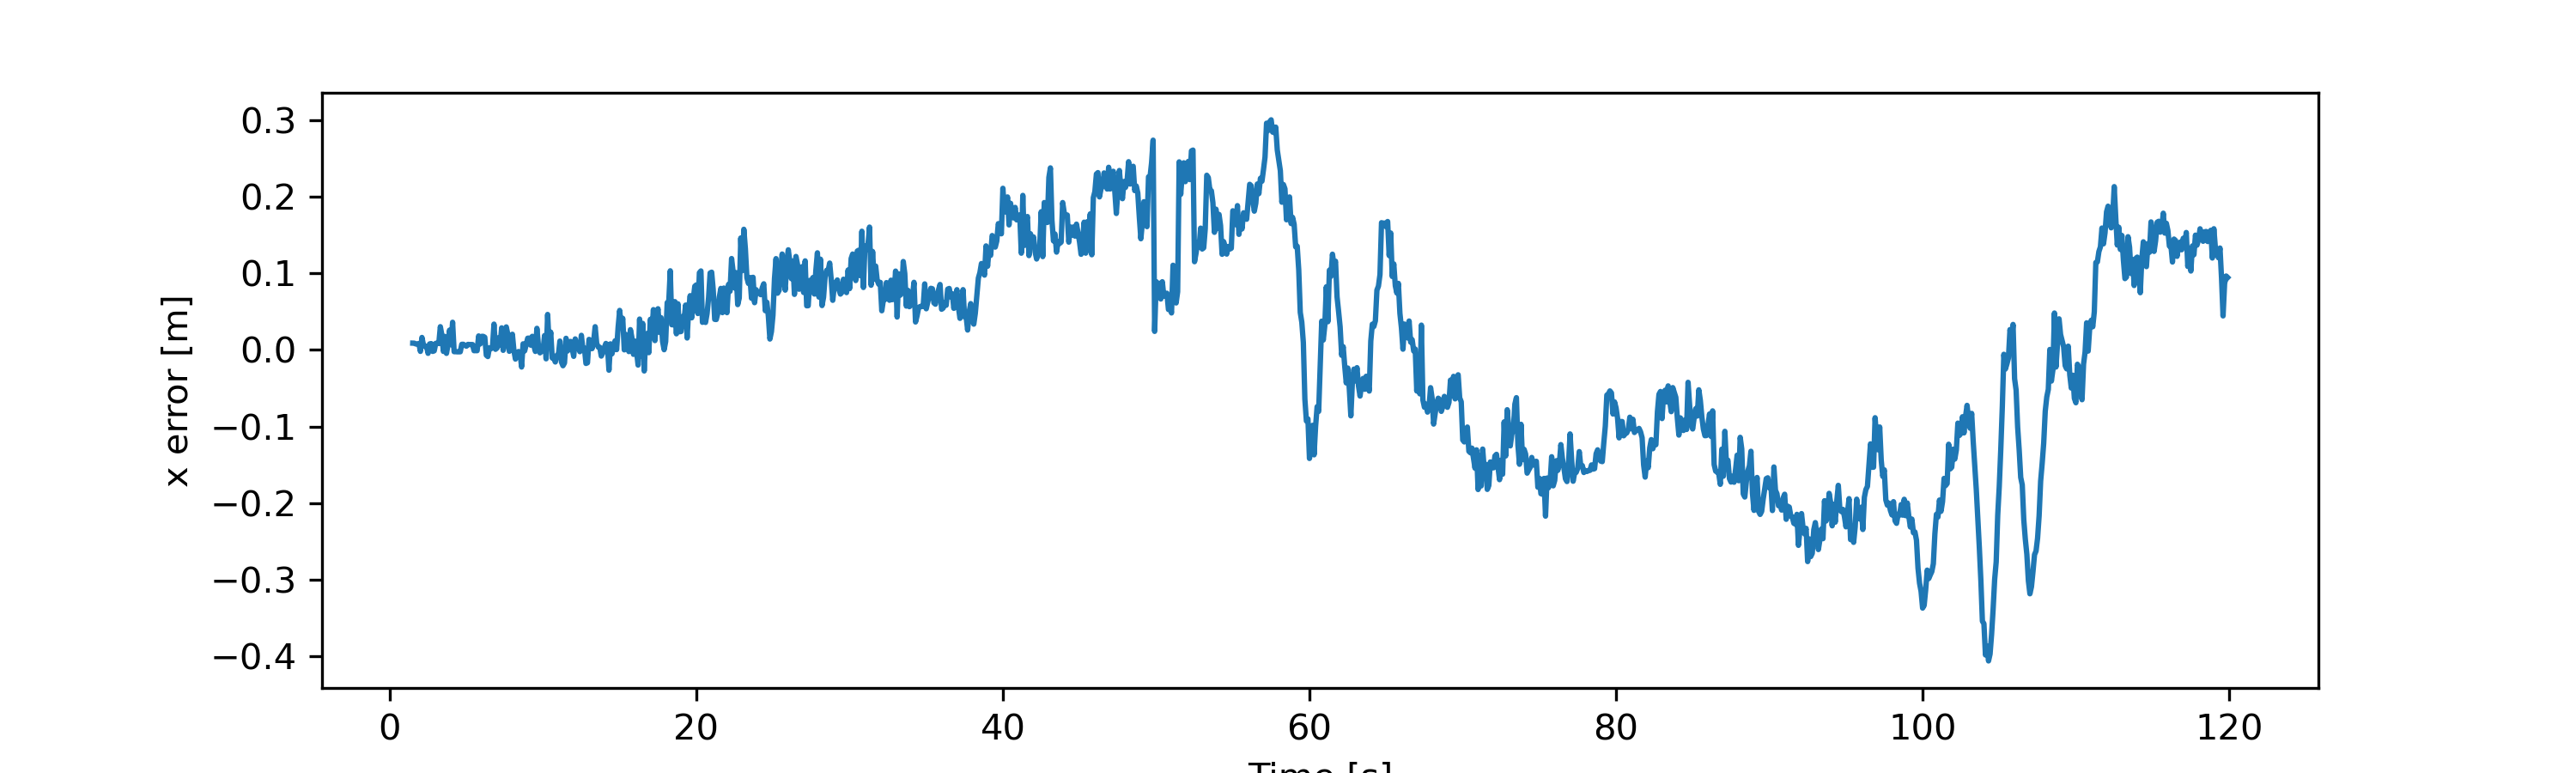
\includegraphics[width=0.48\textwidth]{images/real_test/real_tag_estimation_errx.png}}\\
     \subfigure[]{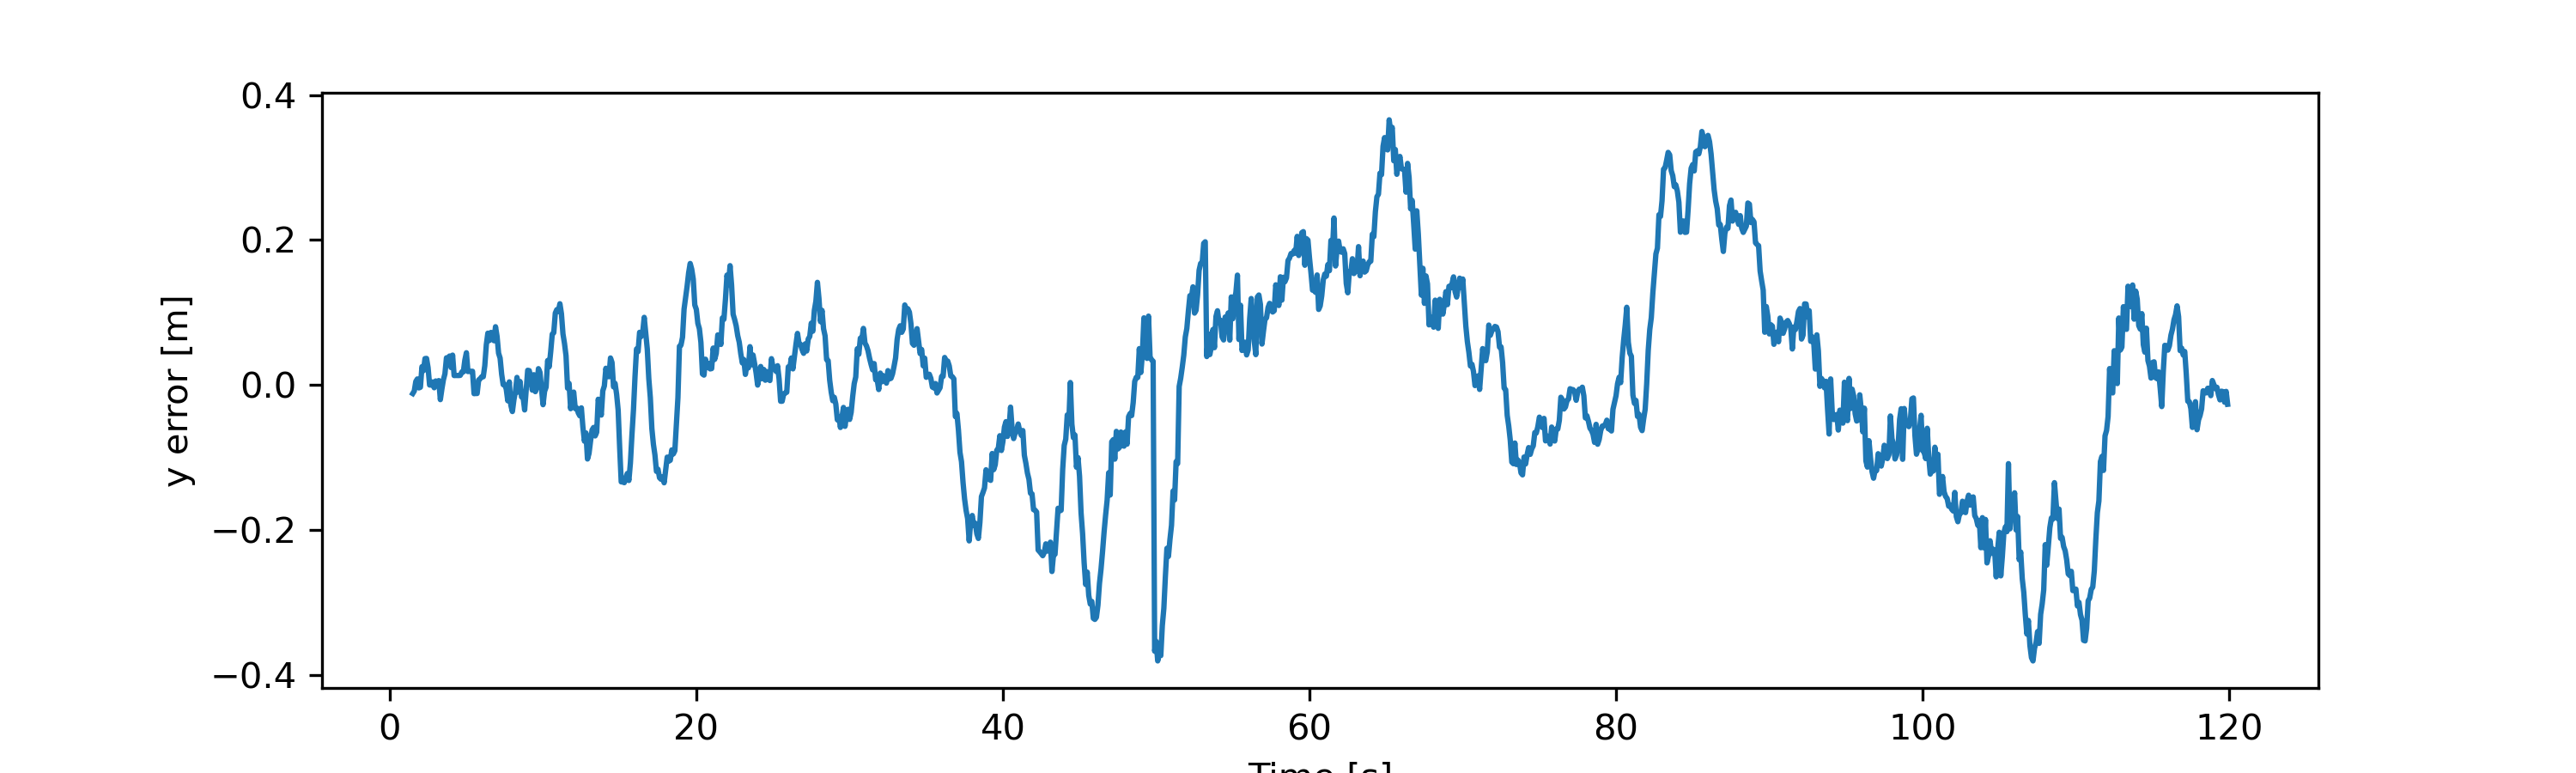
\includegraphics[width=0.48\textwidth]{images/real_test/real_tag_estimation_erry.png}}
     \caption{(a) target localization x error [m]. (b) target localization y error [m].}
     \label{REAL:fig:loc_err}
\end{figure}


\section{Conclusions}\label{CONCLUSIONS}
Our work, through simulations and real tests, has demonstrated and validated the functioning of the developed solution, and the potential of this new type of UWB in the field. Nevertheless, it is clear that there is still room for improvements. In particular, other refinements on the UWB tuning and on its firmware, could provide better target pose estimation and consequently better performances. Indeed, as suggested in \autoref{UWB_CHAR}, modelling the non-linearity of the PDoA w.r.t. the distance, for example developing a proper look up table, could improve the performances and the robustness. From the manufacturing point of view, the development of a pure isotropic target antenna, can improve the measurement performance to, solving the antennas mutual orientation related problems pointed in \autoref{UWB_CHAR} conclusions.\\

For what concerns our strategy, we directly use the measures without filtering and fusion. Investigation in filtering methods that also consider prior information about the motion of the target, are suggested to improve the strategy robustness. Also our PID controller could be better tuned, performing some optimization on the gains.


\let\oldUrl\url
\renewcommand{\url}[2]{\ifx#1\else[\href{#1}{Ref}]\fi}
\bibliographystyle{unsrtnat}
\bibliography{bibliografia}

\end{document}

